\documentclass[11pt,a4paper,twoside]{tesis}
% SI NO PENSAS IMPRIMIRLO EN FORMATO LIBRO PODES USAR
%\documentclass[11pt,a4paper]{tesis}

\usepackage{graphicx}
\usepackage[utf8]{inputenc}
\usepackage[spanish, english]{babel}
\usepackage[left=3cm,right=3cm,bottom=3.5cm,top=3.5cm]{geometry}
\usepackage[usenames]{color}
\usepackage{hyperref}

%configuraciones especiales de paquetes

%\usepackage{todonotes} % si se pone este, no se puede poner el customizado de abajo

%%% todolist
\usepackage{xargs}                      % Use more than one optional parameter in a new commands
\usepackage[pdftex,dvipsnames]{xcolor}  % Coloured text etc.
\usepackage[colorinlistoftodos,prependcaption ]{todonotes} % dentro de corchetes puede ir tmb: ,textsize=tiny 
\newcommandx{\todorevisar}[2][1=]{\todo[inline, linecolor=red,backgroundcolor=red!25,bordercolor=red,#1]{#2}}
\newcommandx{\todocambiar}[2][1=]{\todo[inline, linecolor=blue,backgroundcolor=blue!25,bordercolor=blue,#1]{#2}}
\newcommandx{\todoinfo}[2][1=]{\todo[inline, linecolor=OliveGreen,backgroundcolor=OliveGreen!25,bordercolor=OliveGreen,#1]{#2}}
\newcommandx{\todomejorar}[2][1=]{\todo[inline, linecolor=Plum,backgroundcolor=Plum!25,bordercolor=Plum,#1]{#2}}
\newcommandx{\comentarioinvisible}[2][1=]{\todo[disable,#1]{#2}}

%%% footnotes
\usepackage{sepfootnotes} %http://ctan.dcc.uchile.cl/macros/latex/contrib/sepfootnotes/sepfootnotes.pdf
\newfootnotes{b}

\bnotecontent{GIAR}{giarrrrr}
%%%


%configuraciones para tablas
\usepackage{booktabs}
\usepackage{colortbl}
\usepackage{longtable}

% configuracion para inclir r notebooks
\usepackage{listings} %por pandoc dsps borrar
%\usepackage{framed, graphicx, xcolor}

\usepackage{xcolor}


\definecolor{codegreen}{rgb}{0,0.6,0}
\definecolor{codegray}{rgb}{0.5,0.5,0.5}
\definecolor{codepurple}{rgb}{0.58,0,0.82}
\definecolor{backcolour}{rgb}{0.95,0.95,0.92}

\lstdefinestyle{mystyle}{
	backgroundcolor=\color{backcolour},   
	commentstyle=\color{codegreen},
	keywordstyle=\color{magenta},
	numberstyle=\tiny\color{codegray},
	stringstyle=\color{codepurple},
	basicstyle=\ttfamily\footnotesize,
	breakatwhitespace=false,         
	breaklines=true,                 
	captionpos=b,                    
	keepspaces=true,                 
	numbers=left,                    
	numbersep=5pt,                  
	showspaces=false,                
	showstringspaces=false,
	showtabs=false,                  
	tabsize=2
}

\lstset{style=mystyle}

%%%%%%%%%%%%%%%%%%%%%%%%%%%%%%%%%%%%%%%%%

\begin{document}


%%%% CARATULA

\def\autor{Ing. Sebastian Ezequiel Jaremczuk}
\def\tituloTesis{Deserción en Carreras de Ingeniería: \vspace{.2cm} Análisis y Descubrimiento de posibles causas}
\def\runtitulo{Deserción en Carreras de Ingeniería: Análisis de posibles causas}

\def\director{Mg. Ing. Juan Carlos Gómez}
\def\codirector{Dr. Marcelo Soria}
\def\lugar{Buenos Aires, 2020}
\newcommand{\HRule}{\rule{\linewidth}{0.2mm}}
%
\thispagestyle{empty}

\begin{center}\leavevmode

\vspace{-2cm}

\begin{tabular}{l}

\includegraphics[width=4cm]{caratula/logofcen.pdf}
\end{tabular}

{\large \sc Universidad de Buenos Aires

Facultad de Ciencias Exactas y Naturales}


\begin{tabular}{l}

\includegraphics[width=4cm]{caratula/logo_UBA_DM.jpeg}
\end{tabular}

{\large \sc Maestría en Explotación de Datos y Descubrimiento del Conocimiento}


\vspace{4.0cm}

%\vspace{3.0cm}
%{
%\Large \color{red}
%\begin{tabular}{|p{2cm}cp{2cm}|}
%\hline
%& Pre-Final Version: \today &\\
%\hline
%\end{tabular}
%}
%\vspace{2.5cm}

\begin{huge}
\textbf{\tituloTesis}
\end{huge}

\vspace{2cm}

{\large Trabajo de Especialización}

\vspace{2cm}

{\Large \autor}

\end{center}

\vfill

{\large

%{Director: \director}

\vspace{.2cm}

{Revisor: \codirector}

\vspace{.2cm}

\lugar
}

\newpage\thispagestyle{empty}


%%%% ABSTRACTS, AGRADECIMIENTOS Y DEDICATORIA
\frontmatter
\pagestyle{empty}
%\begin{center}
%\large \bf \runtitulo
%\end{center}
%\vspace{1cm}
\chapter*{\runtitulo}

\noindent El presente trabajo expone la investigación realizada sobre datos de estudiantes de la UTN\bnote{UTN} con el fin de tratar de identificar cuales son las características o patrones de comportamiento que corresponden a estudiantes con altas probabilidades de que en un futuro abandonen sus estudios, convirtiéndose en desertores de la carrera de ingeniería. El enfoque de análisis propuesto es mediante un análisis exploratorio inicial para la comprensión de los datos y posteriormente la aplicación de técnicas que se encuadran dentro del campo de la minería de datos. Puede concluirse que es factible la detección temprana de posibles futuros estudiantes desertores habiendo obtenido entre un 75\% y un 85\% de casos acertados, dependiendo si se seleccionan modelos que sean explicativos o no. Por último, este proceso se realizó siguiendo la Metodología CRISP-DM lo que asegura la reproducibilidad de este trabajo y extensiva documentación de cada paso del proyecto.
\comentarioinvisible{\textcolor{red}{(aprox. 200 palabras)}.!!}

\bigskip

\noindent\textbf{Palabras claves:} Minería de Datos, cluster, árbol de decisión, Gradient Boosting Machine (GBM), RandomForest, Regresión Logística, SVM, R, Python.





%\cleardoublepage
%%\begin{center}
%\large \bf \runtitle
%\end{center}
%\vspace{1cm}
\chapter*{\runtitle}

\noindent In a galaxy far, far away, a psychopathic emperor and his most trusted servant -- a former Jedi Knight known as Darth Vader -- are ruling a universe with fear. They have built a horrifying weapon known as the Death Star, a giant battle station capable of annihilating a world in less than a second. When the Death Star's master plans are captured by the fledgling Rebel Alliance, Vader starts a pursuit of the ship carrying them. A young dissident Senator, Leia Organa, is aboard the ship \& puts the plans into a maintenance robot named R2-D2. Although she is captured, the Death Star plans cannot be found, as R2 \& his companion, a tall robot named C-3PO, have escaped to the desert world of Tatooine below. Through a series of mishaps, the robots end up in the hands of a farm boy named Luke Skywalker, who lives with his Uncle Owen \& Aunt Beru. Owen \& Beru are viciously murdered by the Empire's stormtroopers who are trying to recover the plans, and Luke \& the robots meet with former Jedi Knight Obi-Wan Kenobi to try to return the plans to Leia Organa's home, Alderaan. After contracting a pilot named Han Solo \& his Wookiee companion Chewbacca, they escape an Imperial blockade. But when they reach Alderaan's coordinates, they find it destroyed - by the Death Star. They soon find themselves caught in a tractor beam \& pulled into the Death Star. Although they rescue Leia Organa from the Death Star after a series of narrow escapes, Kenobi becomes one with the Force after being killed by his former pupil - Darth Vader. They reach the Alliance's base on Yavin's fourth moon, but the Imperials are in hot pursuit with the Death Star, and plan to annihilate the Rebel base. The Rebels must quickly find a way to eliminate the Death Star before it destroys them as it did Alderaan (aprox. 200 palabras).

\bigskip

\noindent\textbf{Keywords:} War, Rebellion, Wookie, Jedi, The Force, Empire (no menos de 5). % OPCIONAL: comentar si no se quiere

\cleardoublepage
\chapter*{Agradecimientos}

\noindent Al Grupo de Inteligencia Artificial y Robótica de la Universidad Tecnológica Nacional Facultad Regional Buenos Aires (GIAR-UTN-FRBA\bnote{GIAR}) y a todo su equipo por aceptarme en su espacio y dejarme formar parte de este proyecto de investigación.
 % OPCIONAL: comentar si no se quiere

%\cleardoublepage
%\hfill \textit{A mi persona favorita.}
  % OPCIONAL: comentar si no se quiere

\cleardoublepage
\tableofcontents

\mainmatter
\pagestyle{headings}

%%%% CONTENIDO DE LA TESIS

%\todorevisar{revisar. ejemplo de todolist}
%\todocambiar{cambiar. ejemplo de todolist}
%\todoinfo{info. ejemplo de todolist}
%\todomejorar{mejorar. ejemplo de todolist}
%\todohacer{hacer, ejemplo de todolist}
%
%
%\section{pruebas}


si escribimos algo aca

\begin{table}[!h]

\caption{\label{tab:tabla_Dataset_Alumnos}Campos Tabla Alumnos}
\centering
\fontsize{10}{12}\selectfont
\begin{tabular}[t]{ll}
\toprule
\multicolumn{1}{c}{Dataset Alumnos} & \multicolumn{1}{c}{Observaciones: 8335} \\
\cmidrule(l{3pt}r{3pt}){1-1} \cmidrule(l{3pt}r{3pt}){2-2}
\rowcolor{black}  \multicolumn{1}{c}{\textcolor{white}{\textbf{variable}}} & \multicolumn{1}{c}{\textcolor{white}{\textbf{tipo}}}\\
\midrule
\rowcolor{gray!6}  Codigo.Alumno & integer\\
Pais & character\\
\rowcolor{gray!6}  Localidad & character\\
Provincia & character\\
\rowcolor{gray!6}  Estudios.Secundarios & character\\
\addlinespace
Estado.Civil & character\\
\bottomrule
\end{tabular}
\end{table}

\begin{table}[!h]

\caption{\label{tab:tabla_Dataset_Cursadas}Campos Tabla Cursadas}
\centering
\fontsize{10}{12}\selectfont
\begin{tabular}[t]{ll}
\toprule
\multicolumn{1}{c}{Dataset Cursadas} & \multicolumn{1}{c}{Observaciones: 199815} \\
\cmidrule(l{3pt}r{3pt}){1-1} \cmidrule(l{3pt}r{3pt}){2-2}
\rowcolor{black}  \multicolumn{1}{c}{\textcolor{white}{\textbf{variable}}} & \multicolumn{1}{c}{\textcolor{white}{\textbf{tipo}}}\\
\midrule
\rowcolor{gray!6}  Codigo.Alumno & double\\
Sexo & character\\
\rowcolor{gray!6}  Año.de.ingreso & double\\
Año.de.nacimiento & double\\
\rowcolor{gray!6}  Curso & character\\
\addlinespace
Materia & character\\
\rowcolor{gray!6}  Departamento & character\\
Modalidad & character\\
\rowcolor{gray!6}  Turno & character\\
Ciclo.Lectivo.de.Cursada & double\\
\addlinespace
\rowcolor{gray!6}  Tipo.de.aprobación & character\\
Cantidad.de.veces.recursada.regular & double\\
\rowcolor{gray!6}  Descripción.de.recursada.regular & character\\
Cantidad.de.veces.recursada.libre & double\\
\rowcolor{gray!6}  Descripción.de.recursada.libre & character\\
\bottomrule
\end{tabular}
\end{table}

\begin{table}[!h]

\caption{\label{tab:tabla_Dataset_Finales}Campos Tabla Finales}
\centering
\fontsize{10}{12}\selectfont
\begin{tabular}[t]{ll}
\toprule
\multicolumn{1}{c}{Dataset Finales} & \multicolumn{1}{c}{Observaciones: 83291} \\
\cmidrule(l{3pt}r{3pt}){1-1} \cmidrule(l{3pt}r{3pt}){2-2}
\rowcolor{black}  \multicolumn{1}{c}{\textcolor{white}{\textbf{variable}}} & \multicolumn{1}{c}{\textcolor{white}{\textbf{tipo}}}\\
\midrule
\rowcolor{gray!6}  Codigo.Alumno & character\\
Materia & character\\
\rowcolor{gray!6}  Año & character\\
Nota & character\\
\rowcolor{gray!6}  Aprobado & character\\
\addlinespace
Promociono & character\\
\bottomrule
\end{tabular}
\end{table}



\begin{table}[!h]

\caption{\label{tab:tabla_Alumnos_Estadisticos_Categoricos}Tabla Alumnos, valores mas frecuentes}
\centering
\fontsize{10}{12}\selectfont
\begin{tabular}[t]{llrrr}
\toprule
\rowcolor{black}  \multicolumn{1}{c}{\textcolor{white}{\textbf{variable}}} & \multicolumn{1}{c}{\textcolor{white}{\textbf{característica}}} & \multicolumn{1}{c}{\textcolor{white}{\textbf{frecuencia}}} & \multicolumn{1}{c}{\textcolor{white}{\textbf{frecuencia\_pct}}} & \multicolumn{1}{c}{\textcolor{white}{\textbf{rank}}}\\
\midrule
\rowcolor{gray!6}  Pais & Argentina & 8242 & 98.88 & 1\\
Pais & Perú & 33 & 0.40 & 2\\
\rowcolor{gray!6}  Pais & Bolivia & 22 & 0.26 & 3\\
Localidad & Ciudad Autónoma de Buenos Aires & 3767 & 45.19 & 1\\
\rowcolor{gray!6}  Localidad & Lomas de Zamora & 163 & 1.96 & 2\\
\addlinespace
Localidad & Lanús Oeste & 124 & 1.49 & 3\\
\rowcolor{gray!6}  Provincia & CABA / Capital Federal & 5744 & 68.91 & 1\\
Provincia & BUENOS AIRES & 2183 & 26.19 & 2\\
\rowcolor{gray!6}  Provincia & NA & 88 & 1.06 & 3\\
Estudios.Secundarios & Bachiller & 3557 & 42.68 & 1\\
\addlinespace
\rowcolor{gray!6}  Estudios.Secundarios & Técnico & 2139 & 25.66 & 2\\
Estudios.Secundarios & NA & 1089 & 13.07 & 3\\
\rowcolor{gray!6}  Estado.Civil & SOLTERO & 8182 & 98.16 & 1\\
Estado.Civil & CASADO & 118 & 1.42 & 2\\
\rowcolor{gray!6}  Estado.Civil & NA & 19 & 0.23 & 3\\
\bottomrule
\end{tabular}
\end{table}





\hypertarget{TOC}{}

\hypertarget{header}{}
\hypertarget{sample-document}{%
	\section{Sample Document}\label{sample-document}}

\hypertarget{sebastian-jaremczuk}{%
	\paragraph{Sebastian Jaremczuk}\label{sebastian-jaremczuk}}

\hypertarget{section}{%
	\paragraph{2020-03-31}\label{section}}

\hypertarget{titu}{}
\hypertarget{titu}{%
	\subsection{titu}\label{titu}}

\begin{lstlisting}[language=R]
print("notebook")
\end{lstlisting}

\begin{lstlisting}
## [1] "notebook"
\end{lstlisting}

\hypertarget{lo}{}
\hypertarget{lo}{%
	\section{lo}\label{lo}}

\begin{lstlisting}[language=R]
print("2ndo chunk")
\end{lstlisting}

\begin{lstlisting}
## [1] "2ndo chunk"
\end{lstlisting}


%%%%%%%%%%
%
%\definecolor{shadecolor}{gray}{0.9}
%
%%%%%
%
%\hypertarget{TOC}{}
%
%\hypertarget{header}{}
%\hypertarget{sample-document}{%
%	\section{Sample Document}\label{sample-document}}
%
%\hypertarget{sebastian-jaremczuk}{%
%	\paragraph{Sebastian Jaremczuk}\label{sebastian-jaremczuk}}
%
%\hypertarget{section}{%
%	\paragraph{2020-03-31}\label{section}}
%
%\hypertarget{titu}{}
%\hypertarget{titu}{%
%	\subsection{titu}\label{titu}}
%
%\begin{shaded}
%	\begin{Highlighting}[]
%		\KeywordTok{print}\NormalTok{(}\StringTok{"notebook"}\NormalTok{)}
%	\end{Highlighting}
%\end{shaded}
%
%\begin{verbatim}
%## [1] "notebook"
%\end{verbatim}
%
%\hypertarget{lo}{}
%\hypertarget{lo}{%
%	\section{lo}\label{lo}}
%
%\begin{Shaded}
%	\begin{Highlighting}[]
%		\KeywordTok{print}\NormalTok{(}\StringTok{"2ndo chunk"}\NormalTok{)}
%	\end{Highlighting}
%\end{Shaded}
%
%\begin{verbatim}
%## [1] "2ndo chunk"
%\end{verbatim}






%%%% DOMINIO
%-------------------------------------------------%
\chapter{Comprensión del Dominio}
%-------------------------------------------------%
%-------------------------------------------------%
\section{Determinar Objetivos}
%-------------------------------------------------%
%-------------------------------------------------%
\subsection{Información general del dominio}
%-------------------------------------------------%
\subsubsection{La Deserción}\label{seccion:desercion}
En todo el campo educativo, un fenómeno recurrente y de los más relevantes es el de la deserción. Está presente en todos los niveles educativos. Las Universidades no parecen ser la excepción y, de distintas maneras y por distintos motivos, buscaron y buscan una manera de entenderlo. En primer lugar no existe una definición única y que abarque completamente del complejo fenómeno de la deserción.  
Viale Tudela \cite{ErnestoUNAOUT} recoge ciertos intentos de captar estas "intuiciones", en las cuales la idea generalizada apunta hacia el cese de actividades deliberado o forzado del alumno en la institución educadora, pero que no todo cese de actividades representa una
verdadera deserción. En el Glosario de Términos Básicos \cite{CONEAU2010PropuestaSINEACE}, el CONEAU (Perú) recurre a una definición como “proceso de abandono, voluntario o forzoso, de la carrera en la que se matricula un estudiante, por la influencia positiva o negativa de circunstancias internas o externas a él o ella”, pero no suprime la dimensión cuantitativa como una proporción relativa a la duración de las carreras. Aparecen así otros conceptos ligados a la deserción, como la cronicidad y el desgranamiento. El Desgranamiento es el fenómeno por el cual ciertos alumnos de una cohorte -si bien conservan su condición de regularidad- no cumplen con los plazos del plan de estudios de la carrera. La cronicidad describe la situación de alumnos o carreras con altos índices de desgranamiento. Y en general la deserción es el fenómeno por el cual los alumnos de una carrera o de una universidad abandonan el cursado de los estudios y como consecuencia no cumplen con las  condiciones de regularidad.

\subsubsection{Antecedentes}
Dada la importancia de este problema, se han buscado distintos métodos para poder dar con  las causas de la deserción universitaria. Uno de ellos es el de identificar rasgos o variables que puedan ser tomados como indicadores relacionados con la emergencia de la deserción. Los trabajos sobre indicadores académicos son numerosos y buena parte se centra en el rendimiento de los estudiantes e incluyen variables culturales, demográficas, laborales, entre otras, además de su historial académico (materias aprobadas, asignación de becas, repitencia, etc.), aunque existen trabajos más integrales que consideran factores socioeconómicos, personales, académicos e institucionales \cite{L.GonzalezFeigehen2006RepitenciaLatina,SociedadModeloSuperior}.
En ocasiones se realizaron propuestas \cite{Kuna2009IdentificacionUniversitarios} para modificar la emergencia de la deserción incidiendo directamente en las variables tomadas como indicadores.



\subsubsection{Estudio de la Deserción: Enfoque desde la Minería de Datos }\label{seccion:dm_en_desercion}
Dentro del campo de Minería de Datos existen una enorme y muy variada cantidad de modelos de análisis. El "Análisis de Desgaste" es uno de ellos. que nacen por parte de las empresas para detectar los fenómenos que generan el comportamiento de la deserción de sus clientes. Se trata de encontrar la relación entre la deserción y las principales variables que afectan a ello. El objetivo del análisis de desgaste es proporcionar al investigador la capacidad de entender qué variables son las más importante al desgaste y cuál es la probabilidad del abandono del cliente. De esta forma es posible entender el porqué y además predecir qué tipo de clientes son más proclives a la deserción. Estas técnicas se usan actualmente también en al ámbito financiero para evaluar qué personas son buenas/malas pagadoras de créditos, en el ámbito de la salud para evaluar el comportamiento de las personas frente a cierta enfermedad y en las empresas para retener clientes o empleados \cite{Chapman1982AttritionAnalysis}.


%-------------------------------------------------%
\subsection{Definir Objetivos}
%-------------------------------------------------%
%# posibles objetivos

\textbf{Objetivo General}\\
\begin{itemize}
	\item El objetivo de este trabajo es ofrecer a los especialistas en educación nuevas herramientas de análisis y descubrimiento de conocimiento sobre el fenómeno de la deserción, y así poder incorporarlas a otros trabajos que busquen modificar la naturaleza y las condiciones de posibilidad del fenómeno.
	\item Inicialmente, se propone analizar fenómenos particulares de deserción, es decir, la deserción en la carrera de ingeniería en sistemas de la UTN-FRBA \bnote{UTN}\bnote{FRBA}.
	\item La intensión también es poder dar el mejor apoyo posible a los alumnos de la Universidad y a la Universidad misma.
\end{itemize}

Por tal motivo, se comenzó con una definición propia, medible y
simple de la situación de deserción definida como: dos años consecutivos sin actividad. Esto es sin cursar ni aprobar finales.


\textbf{Objetivos Particulares}
\begin{itemize}
	\item Desarrollar algoritmos de modelos descriptivos para la explicación de las variables relevantes al problema elegido. Particularmente en este trabajo se estudiará la desersión de los estudiante.
	\item Desarrollar algoritmos de modelos predictivos para evaluar los comportamientos actuales de los estudiantes y brindar los resultados a las personas idóneas para que puedan actuar en consecuencia.
	\item Obtener patrones y evaluar los mismos para crear las reglas y la Base de Conocimiento de un Sistema Experto, mediante el resultado de los patrones obtenidos.
\end{itemize}

\comentarioinvisible{este punto por ahora no lo pongo como objetivo. Desarrollo de un Sistema Experto para evaluar el comportamiento estudiantil a fin de dar soporte a la toma de decisiones.}




%-------------------------------------------------%
\subsection{Definir el criterio de éxito}
%-------------------------------------------------%

\todorevisar{revisar si el criterio es realizable o no}

Éxito:
\begin{itemize}
\item clasificar correctamente mas del 90\% a los alumnos que van a desertar.
\item clasificar correctamente mas de 80 \% a los alumnos en general (desertores o no)
\item poder explicar al menos 2 características (variables) encontradas a través de los análisis.
\end{itemize}

%-------------------------------------------------%
%-------------------------------------------------%
\section{Evaluar la situación}
%-------------------------------------------------%
%-------------------------------------------------%
\subsection{Recursos}
%-------------------------------------------------%
De forma de garantizar la total reproducción de este trabajo con incluso los mismo resultados de análisis independientemente de quién lo realice, dónde se lo realice y bajo qué requerimientos computacionales, se tomó la decisión de armar un ambiente de trabajo propio y portable, el cual contiene todas las herramientas de software necesarias y configuradas. A su vez, se registra todo avance realizado históricamente con sus modificaciones y código fuente para su ejecución.

Esto se pudo realizar armando previamente al análisis una infraestructura. La misma se compone de:

\begin{itemize}
\item \href{https://www.docker.com/}{\textcolor{blue}{\underline{Docker}}}
\item Linux, \href{https://ubuntu.com/}{\textcolor{blue}{\underline{Ubuntu}}}
\item \href{ https://www.r-project.org/}{\textcolor{blue}{\underline{R}}}, \href{https://rstudio.com/}{\textcolor{blue}{\underline{Rstudio}}}
\item \href{https://www.python.org/}{\textcolor{blue}{\underline{Python}}}
\item \href{https://code.visualstudio.com/}{\textcolor{blue}{\underline{Visual Studio Code}}}
\item \href{https://jupyter.org/}{\textcolor{blue}{\underline{Jupyter}}} 
\item \href{https://git-scm.com/}{\textcolor{blue}{\underline{git}}} con metodología \href{https://github.com/nvie/gitflow}{\textcolor{blue}{\underline{gitflow}}}
\item \href{http://projecttemplate.net/index.html}{\textcolor{blue}{\underline{ProjectTemplate}}} 
\end{itemize}


\includegraphics[width=2cm]{imagenes/logos/docker.jpeg}

\includegraphics[width=2cm]{imagenes/logos/ubuntu_logo_2.png}

\includegraphics[width=2cm]{imagenes/logos/Rlogo.png}

\includegraphics[width=2cm]{imagenes/logos/python.jpeg}

\includegraphics[width=2cm]{imagenes/logos/jupyter.png}

\includegraphics[width=2cm]{imagenes/logos/git_logo_2.png}

\vspace{5mm}


\paragraph{NOTA:}
La reproducción es factible si la persona tiene acceso y cuenta con la información de la base de datos con la que se realizó este trabajo que por cuestiones de confidencialidad mencionadas anteriormente no serán entregadas.



%-------------------------------------------------%
\subsection{Requerimientos, supuestos, condicionantes}
%-------------------------------------------------%

\subsubsection{\textcolor{red}{Requerimientos}}
Es de suma importancia destacar la toma de conciencia para incorporar en las instituciones educativas sistemas que permitan el registro de cada vez más variedad de variables y de distinto tipo respecto de los contextos nombrados anteriormente de los estudiantes.
Esta conformación de bases de datos es imprescindible para este tipo de trabajos, por lo que todo trabajo que esté interesado en realizar un estudio sobre el fenómeno de la deserción, debe contar con ella como si fuera su material de trabajo inicial.
A partir de la toma de conciencia sobre la necesidad de contar con estas complejas bases de datos es que se pueden aplicar las técnicas de Data Mining y es de esperar que se tenga éxito de la misma manera en que se obtienen en otros campos como el de la medicina \cite{Adnan2013DataReview}, marketing, o el bancario\cite{Kirkos2007DataStatements}.


\subsubsection{Condicionantes}
Ética en el uso responsable de la información y de confidencialidad.
Al tratarse de datos de alumnos de la Universidad, su desenvolvimiento académico, entre otro tipo de información. El GIAR \bnote{GIAR} firmó un acuerdo de confidencialidad para la realización de este trabajo y otros relacionados. A su vez, se tomaron medidas para evitar que los investigadores pudiera identificar a alumnos. Algunas de las medias adoptadas fueron reemplazar el nombre por un identificador (ID) de cada alumno y que se
eliminen algunos datos personales.
Además, los datos con los que se trabajan son una muestra representativa de todo el universo.
De esta forma, se crea un ambiente de trabajo seguro y anónimo.

%-------------------------------------------------%
\subsection{Condiciones de riesgo y contingencias}
%-------------------------------------------------%
% que el estudio lo usen para univerisdaddes de elite o para malos usos



Es importante destacar las consecuencias que pudiera tener el ``buen" o ``mal" uso de la información subyacente y a priori desconocida en los datos analizados. Por ejemplo, conocer algunas posibles causas de la deserción, así como el perfil de un potencial desertor puede llevar a un desarrollo de políticas universitarias
que busquen estimular la continuidad en los estudios o por el contrario desalentarla
cuanto antes. Esto puede llevarse a cabo con independencia de si se individualiza
efectivamente o no al estudiante que sea un potencial desertor. Pero si además se lo
identifica, esas políticas podrían ser personalizadas, complementándolas con
entrevistas, cursos de apoyo o asistencia de un tutor. \\
La identificación temprana de algún patrón o característica particular podría ser beneficiosa para el estudiante y para la Universidad. Sin embargo, también habría que considerar el riesgo que conlleva utilizar esos datos, por ejemplo, convertir la casa de estudios en una Universidad elitista.\\
Más allá de trabajar sobre la posibilidad técnica de encontrar información relevante
subyacente en los datos de los estudiantes está claro que hay que considerar los
aspectos éticos antes de cualquier uso que pudiera dárseles. Es evidentemente un
problema complejo con múltiples aristas y con muchas preguntas por responder.


%-------------------------------------------------%
\subsection{terminología}
%-------------------------------------------------%
\textbf{UTN:} Universidad Tecnológica Nacional
\textbf{FRBA:} Facultad Regional Buenos Aires

DM: Data Mining - Minería de Datos
RLog: Regresión Logística


%-------------------------------------------------%
\subsection{Determinar costos y beneficios}
%-------------------------------------------------%
No aplica.
%-------------------------------------------------%
%-------------------------------------------------%
\section{Objetivos de data mining}
%-------------------------------------------------%
%-------------------------------------------------%
\subsection{Determinar los objetivos}
%-------------------------------------------------%
%# posibles objetivos

\textbf{Objetivo General}\\
\begin{itemize}
	\item El objetivo de este trabajo es ofrecer a los especialistas en educación nuevas herramientas de análisis y descubrimiento de conocimiento sobre el fenómeno de la deserción, y así poder incorporarlas a otros trabajos que busquen modificar la naturaleza y las condiciones de posibilidad del fenómeno.
	\item Inicialmente, se propone analizar fenómenos particulares de deserción, es decir, la deserción en la carrera de ingeniería en sistemas de la UTN-FRBA \bnote{UTN}\bnote{FRBA}.
	\item La intensión también es poder dar el mejor apoyo posible a los alumnos de la Universidad y a la Universidad misma.
\end{itemize}

Por tal motivo, se comenzó con una definición propia, medible y
simple de la situación de deserción definida como: dos años consecutivos sin actividad. Esto es sin cursar ni aprobar finales.


\textbf{Objetivos Particulares}
\begin{itemize}
	\item Desarrollar algoritmos de modelos descriptivos para la explicación de las variables relevantes al problema elegido. Particularmente en este trabajo se estudiará la desersión de los estudiante.
	\item Desarrollar algoritmos de modelos predictivos para evaluar los comportamientos actuales de los estudiantes y brindar los resultados a las personas idóneas para que puedan actuar en consecuencia.
	\item Obtener patrones y evaluar los mismos para crear las reglas y la Base de Conocimiento de un Sistema Experto, mediante el resultado de los patrones obtenidos.
\end{itemize}

\comentarioinvisible{este punto por ahora no lo pongo como objetivo. Desarrollo de un Sistema Experto para evaluar el comportamiento estudiantil a fin de dar soporte a la toma de decisiones.}




%-------------------------------------------------%
\subsection{Definir el criterio de éxito}
%-------------------------------------------------%

\todorevisar{revisar si el criterio es realizable o no. JuanCa sombreò 90\% y puso que sea sensible ... nose a que se refiere. Hoy esta en un 88.2\% de clasificacion correcta de desertores asique poner 85 estaría bien si es que se quiere cumplir}

Éxito:
\begin{itemize}
	\item clasificar correctamente mas del 85\% a los alumnos que van a desertar.
	\item clasificar correctamente mas de 80 \% a los alumnos en general (desertores o no)
	\comentarioinvisible{
	\item poder explicar al menos 2 características (variables) encontradas a través de los análisis. \todorevisar{descartado. borrar o cambiar}}
\end{itemize}
%-------------------------------------------------%
%-------------------------------------------------%
\section{Producir el plan del proyecto}
%-------------------------------------------------%
%######################
%# importante
%# metodología de trabajo y que se va a hacer con este trabajo

En particular:
Se establecerá un protocolo para la obtención de datos de la base de datos de la facultad acordado con las
autoridades respectivas de manera de preservar el secreto estadístico (la identidad de los estudiantes cuyos datos serán
analizados). La cantidad de datos deberá ser representativa de la población donde se produce el fenómeno.
Se seleccionarán las herramientas más adecuadas al problema y a la base de datos a tratar.
Se realizarán experiencias y se desarrollarán modelos descriptivos y predictivos del comportamiento de los
estudiantes en lo referente al comportamiento seleccionado como ejemplo. Se sintonizarán y/o adecuarán los diferentes
algoritmos utilizados.
Se compararán los resultados obtenidos por los distintos algoritmos.
Con los patrones encontrados y un relevamiento de las variables pertinentes se propondrán las bases de
conocimiento para la construcción de un sistema experto.
Se buscará interacción con un experto u otro grupo del área educativa para ofrecerle los datos y plantear un trabajo
conjunto a futuro.
Se presentarán para publicar trabajos que muestren los resultados obtenidos en los ensayos experimentales, así
como también las apreciaciones teóricas respecto de los marcos conceptuales en los que se trabajó.
%-------------------------------------------------%
\subsection{Redacción del proyecto}
%-------------------------------------------------%
La Redacción y publicación del trabajo se realizará en el marco del Grupo de Investigación de Inteligencia Artificial y Robótica (GIAR \bnote{GIAR}) de la Universidad Tecnológica Nacional (UTN \bnote{UTN}) Facultad Regional Buenos Aires (FRBA \bnote{FRBA}). A su vez, este trabajo se presentará como Trabajo Final de la Especialización en Explotación de Datos y Descubrimiento de Conocimiento de la Universidad
de Buenos Aires.\\
La documentación del proceso se realiza mediante la Metodología CRISP-DM (Cross Industry Standard Process for Data Mining)
%-------------------------------------------------%
\subsection{Evaluación inicial de técnicas y herramientas}
%-------------------------------------------------%
%# modelos de desgaste, churn, 
\comentarioinvisible{técnicas de la bibliografia: regresión logística, redes bayesianas, arboles de decisión}


Como fue mencionado en \ref{seccion:dm_en_desercion}, los análisis mas apropiados desde el enfoque de la minería de datos para realizar una clasificación binaria del fenómeno de deserción son: El análisis de supervivencia y el de desgaste \cite{PredictModel-GarciaVellidoNebot}

\comentarioinvisible{
\todohacer{explciar brevemete las técnicas que se van a usar y porque son adecuadas}}

Las técnicas que se emplean en este análisis son varias. dentro de ella sse encuentran métodos no supervisados y supervisados.\\
Dentro de las técnicas no supervisada, se emplearán clusters (de varios tipos: kmeans, jerárquico, etc) para evaluar si existe tendencia al agrupamiento y luego corroborar si los grupos tienen características relacionadas con el target. \\
Por otro lado, dentro del grupo de las técnicas supervisadas, se emplean técnicas que son explicativas (arboles simples de decisión, regresión logística, LDA) y técnicas que no son explicativas (RandomForest, GradientBoosting, SVM) y que lo mas explicativo que pueden informar en algunos casos es la importancia de los predictores.\\

De forma complementaria, se realizan análisis de reducción de dimensión y análisis de influencia de variables para generar datasets alternativos mas eficientes del que se esta partiendo.\\

Cada técnica se explica brevemente en la sección donde se aplican los modelos.\ref{generacion_modelos}



%%%% DATOS
%-------------------------------------------------%
\chapter{Comprensión de los Datos}
%-------------------------------------------------%
%-------------------------------------------------%
\section{Colección inicial de datos}
%-------------------------------------------------%


Se obtuvo información de la base  de datos de estudiantes de la Universidad Tecnológica Nacional Facultad Regional Buenos Aires. Mas específicamente una muestra representativa de alumnos de la Carrera de Ingeniería en sistemas con plan 2008 entre el año 2008 y 2016.

La información obtenida y el tratamiento previo al inicio del proyecto se condicionó de acuerdo a lo mencionado en \ref{seccion:condicionantes}

\label{datos:raw}
De esta forma, la información inicial parte principalmente de 3 tablas anónimas exportadas a formato csv.

\begin{enumerate}
\item Cursadas-Alumnos-SIGA: que contiene la información del desempeño académico únicamente referido a las cursadas de los estudiantes.
\item Finales-Alumnos-SIGA: que contiene la información del desempeño académico de los estudiantes únicamente en exámenes finales de las materias cursadas.
\item Datos-Alumnos-SIGA: que contiene datos personales de los alumnos. ùnicamente aquellos datos que no atentan contra la identificación de los mismos.
\end{enumerate}



%-------------------------------------------------%
\section{Describir los datos}
%-------------------------------------------------%
\comentarioinvisible{Recordar que no es hacer descriptivo con dlookr sino que es descripción de los campos}


En las tablas \ref{tab:tabla_Dataset_Alumnos}, \ref{tab:tabla_Dataset_Cursadas} y \ref{tab:tabla_Dataset_Finales} puede observarse una mínima descripción sobre la cantidad y con que tipo de información se tiene. 

\vspace{3mm}

\begin{table}[!h]

\caption{\label{tab:tabla_Dataset_Alumnos}Campos Tabla Alumnos}
\centering
\fontsize{10}{12}\selectfont
\begin{tabular}[t]{ll}
\toprule
\multicolumn{1}{c}{Dataset Alumnos} & \multicolumn{1}{c}{Observaciones: 8335} \\
\cmidrule(l{3pt}r{3pt}){1-1} \cmidrule(l{3pt}r{3pt}){2-2}
\rowcolor{black}  \multicolumn{1}{c}{\textcolor{white}{\textbf{variable}}} & \multicolumn{1}{c}{\textcolor{white}{\textbf{tipo}}}\\
\midrule
\rowcolor{gray!6}  Codigo.Alumno & integer\\
Pais & character\\
\rowcolor{gray!6}  Localidad & character\\
Provincia & character\\
\rowcolor{gray!6}  Estudios.Secundarios & character\\
\addlinespace
Estado.Civil & character\\
\bottomrule
\end{tabular}
\end{table}


\begin{table}[!h]

\caption{\label{tab:tabla_Dataset_Cursadas}Campos Tabla Cursadas}
\centering
\fontsize{10}{12}\selectfont
\begin{tabular}[t]{ll}
\toprule
\multicolumn{1}{c}{Dataset Cursadas} & \multicolumn{1}{c}{Observaciones: 199815} \\
\cmidrule(l{3pt}r{3pt}){1-1} \cmidrule(l{3pt}r{3pt}){2-2}
\rowcolor{black}  \multicolumn{1}{c}{\textcolor{white}{\textbf{variable}}} & \multicolumn{1}{c}{\textcolor{white}{\textbf{tipo}}}\\
\midrule
\rowcolor{gray!6}  Codigo.Alumno & double\\
Sexo & character\\
\rowcolor{gray!6}  Año.de.ingreso & double\\
Año.de.nacimiento & double\\
\rowcolor{gray!6}  Curso & character\\
\addlinespace
Materia & character\\
\rowcolor{gray!6}  Departamento & character\\
Modalidad & character\\
\rowcolor{gray!6}  Turno & character\\
Ciclo.Lectivo.de.Cursada & double\\
\addlinespace
\rowcolor{gray!6}  Tipo.de.aprobación & character\\
Cantidad.de.veces.recursada.regular & double\\
\rowcolor{gray!6}  Descripción.de.recursada.regular & character\\
Cantidad.de.veces.recursada.libre & double\\
\rowcolor{gray!6}  Descripción.de.recursada.libre & character\\
\bottomrule
\end{tabular}
\end{table}


\begin{table}[!h]

\caption{\label{tab:tabla_Dataset_Finales}Campos Tabla Finales}
\centering
\fontsize{10}{12}\selectfont
\begin{tabular}[t]{ll}
\toprule
\multicolumn{1}{c}{Dataset Finales} & \multicolumn{1}{c}{Observaciones: 83291} \\
\cmidrule(l{3pt}r{3pt}){1-1} \cmidrule(l{3pt}r{3pt}){2-2}
\rowcolor{black}  \multicolumn{1}{c}{\textcolor{white}{\textbf{variable}}} & \multicolumn{1}{c}{\textcolor{white}{\textbf{tipo}}}\\
\midrule
\rowcolor{gray!6}  Codigo.Alumno & character\\
Materia & character\\
\rowcolor{gray!6}  Año & character\\
Nota & character\\
\rowcolor{gray!6}  Aprobado & character\\
\addlinespace
Promociono & character\\
\bottomrule
\end{tabular}
\end{table}


\vspace{3mm}

Como puede observarse, algunos campos en primera instancia están categorizadas como tipo de dato \textit{character}, cuando en realidad algunos deberían ser del tipo \textit{numeric} o \textit{factor}.
Esto puede deberse a posibles errores que aparecen en los contenidos de dichos campos o malas transformaciones realizadas previo a que recibir estos datos. Estos temas se tratarán en los siguientes puntos.
\\
Si bien el nombre de algunos campos explican bien el contenido que tienen, algunas pueden llegar a no ser tan claras y a continuación se procede a explicarlas.


\begin{enumerate}
	\item Tabla Cursadas
	\begin{enumerate}
		\item Departamento: Una carrera tiene un plan de estudio compuesto por materias. Estas se dictan en distintos Departamentos, la gran mayoría son del departamento de la carrera que se está cursando pero también hay materias que dependen de otro departamento como lo son por ejemplo las de ciencias básicas.
		\item Modalidad: indica en que momento del año se cursa, cuatrimestras o anual generalmente.
		\item Turno: existen 3 momentos del día para dictar una materia, mañana, tarde y noche.
		\item Ciclo.Lectivo.de.Cursada: año en el que se cursó la materia que hace referencia.
		\item Tipo.de.aprobación: a pesar de hacer referencia a la aprobación, este campo también indica si en el momento que se tomó el registro estaba cursando o no había firmado la materia.
		\item Cantidad.de.veces.recursada.regular: indica el número actual (al momento de tomar ese registro) por el que el alumno esta recursando la materia de referencia.
		\item Descripción.de.recursada.regular: descripción del significado del registro anterior.
	\end{enumerate}
	\item Tabla Finales
	\begin{enumerate}
		\item Aprobado: flag si aprobó o no
		\item Promociono: flag si promocionó o no
	\end{enumerate}
\end{enumerate}




\comentarioinvisible{
El contenido de la base de datos se puede clasificar como sigue:
-Datos personales:
Código Alumno*; Nacionalidad; Sexo, Localidad; Provincia;
Estudios Secundarios, Año de nacimiento y Estado Civil.
-Datos de la cursada:
Código Alumno, Año de ingreso, Curso, Materia, Departamento,
Modalidad, Turno, Ciclo Lectivo de Cursada, Tipo de aprobación,
Cantidad de veces recursada regular, Descripción de recursada
regular, Cantidad de veces recursada libre, Descripción de
recursada libre.
-Datos de Finales:
Código Alumno, Materia, Año, Nota, Aprobado, Promocionó
}
%-------------------------------------------------%
\section{Exploración de datos}\label{exploracion_datos}
%-------------------------------------------------%
\comentarioinvisible{formateo de los datos para dsps hacer analsis estadistico  descriptivo con dlookr, y algunos graficos. ojo! es una exploracion inicial. Hay descriptivos que con para la seccion de calidad de datos}

\subsubsection{Análisis estadísticos generales}

Si bien el los trabajos de calidad de datos se muestran en la siguiente sección, es necesario hacer un mínimo formateo de los datos para poder hacer una exploración inicial.

Las nuevas tablas formateadas son las siguientes \ref{tab:tabla_Alumnos_Estadisticos_Categoricos},  :

\begin{table}[!h]

\caption{\label{tab:tabla_Alumnos_Estadisticos_Categoricos}Tabla Alumnos, valores mas frecuentes}
\centering
\fontsize{10}{12}\selectfont
\begin{tabular}[t]{llrrr}
\toprule
\rowcolor{black}  \multicolumn{1}{c}{\textcolor{white}{\textbf{variable}}} & \multicolumn{1}{c}{\textcolor{white}{\textbf{característica}}} & \multicolumn{1}{c}{\textcolor{white}{\textbf{frecuencia}}} & \multicolumn{1}{c}{\textcolor{white}{\textbf{frecuencia\_pct}}} & \multicolumn{1}{c}{\textcolor{white}{\textbf{rank}}}\\
\midrule
\rowcolor{gray!6}  Pais & Argentina & 8242 & 98.88 & 1\\
Pais & Perú & 33 & 0.40 & 2\\
\rowcolor{gray!6}  Pais & Bolivia & 22 & 0.26 & 3\\
Localidad & Ciudad Autónoma de Buenos Aires & 3767 & 45.19 & 1\\
\rowcolor{gray!6}  Localidad & Lomas de Zamora & 163 & 1.96 & 2\\
\addlinespace
Localidad & Lanús Oeste & 124 & 1.49 & 3\\
\rowcolor{gray!6}  Provincia & CABA / Capital Federal & 5744 & 68.91 & 1\\
Provincia & BUENOS AIRES & 2183 & 26.19 & 2\\
\rowcolor{gray!6}  Provincia & NA & 88 & 1.06 & 3\\
Estudios.Secundarios & Bachiller & 3557 & 42.68 & 1\\
\addlinespace
\rowcolor{gray!6}  Estudios.Secundarios & Técnico & 2139 & 25.66 & 2\\
Estudios.Secundarios & NA & 1089 & 13.07 & 3\\
\rowcolor{gray!6}  Estado.Civil & SOLTERO & 8182 & 98.16 & 1\\
Estado.Civil & CASADO & 118 & 1.42 & 2\\
\rowcolor{gray!6}  Estado.Civil & NA & 19 & 0.23 & 3\\
\bottomrule
\end{tabular}
\end{table}


De la tabla de los datos de Alumnos \ref{tab:tabla_Alumnos_Estadisticos_Categoricos} que son mas frecuentes a nivel global, podemos observar que no se hay valores que llamen la atención para el enfoque del estudio en cuestión. \\
En resumen: La mayoría de los estudiantes son nacionales, viven cerca a la facultad de concurrencia y son solteros (lo cual es lógico sabiendo que la gran mayoría de los que empiezan la facultad lo hacen a una edad temprana). Este último dato nos hace sospechar que puede ser que la base de datos personales no se actualiza con frecuencia por lo que al manipular estos datos debe hacerse con cuidado.
La educación secundaria es equilibrada.
\\

\begin{table}[!h]

\caption{\label{tab:tabla_Cursadas_Estadisticos_Categoricos}Tabla Cursadas, valores más frecuentes}
\centering
\fontsize{10}{12}\selectfont
\begin{tabular}[t]{llrrr}
\toprule
\rowcolor{black}  \multicolumn{1}{c}{\textcolor{white}{\textbf{variable}}} & \multicolumn{1}{c}{\textcolor{white}{\textbf{característica}}} & \multicolumn{1}{c}{\textcolor{white}{\textbf{frecuencia}}} & \multicolumn{1}{c}{\textcolor{white}{\textbf{frecuencia\_pct}}} & \multicolumn{1}{c}{\textcolor{white}{\textbf{rank}}}\\
\midrule
\rowcolor{gray!6}  Sexo & M & 171335 & 85.75 & 1\\
Sexo & F & 28480 & 14.25 & 2\\
\rowcolor{gray!6}  Curso & K1024 & 3909 & 1.96 & 1\\
Curso & K1043 & 3801 & 1.90 & 2\\
\rowcolor{gray!6}  Curso & K1025 & 3748 & 1.88 & 3\\
\addlinespace
Materia & Análisis Matemático I & 18528 & 9.27 & 1\\
\rowcolor{gray!6}  Materia & Álgebra y Geometría Analítica & 17385 & 8.70 & 2\\
Materia & Matemática Discreta & 16715 & 8.37 & 3\\
\rowcolor{gray!6}  Departamento & SISTEMAS & 101844 & 50.97 & 1\\
Departamento & CS.BS. U.D.B. MATEMATICA & 48267 & 24.16 & 2\\
\addlinespace
\rowcolor{gray!6}  Departamento & CS.BS. U.D.B. FISICA & 14290 & 7.15 & 3\\
Modalidad & Anual & 90208 & 45.15 & 1\\
\rowcolor{gray!6}  Modalidad & Cuat 1/2 & 58496 & 29.28 & 2\\
Modalidad & Cuat 2/2 & 50233 & 25.14 & 3\\
\rowcolor{gray!6}  Turno & Mañana & 84893 & 42.49 & 1\\
\addlinespace
Turno & Noche & 76198 & 38.13 & 2\\
\rowcolor{gray!6}  Turno & Tarde & 38724 & 19.38 & 3\\
Tipo.de.aprobación & Firmo & 67253 & 33.66 & 1\\
\rowcolor{gray!6}  Tipo.de.aprobación & No Firmo & 49360 & 24.70 & 2\\
Tipo.de.aprobación & Libre & 37796 & 18.92 & 3\\
\addlinespace
\rowcolor{gray!6}  Descripción.de.recursada.regular & No Recurso & 152426 & 76.28 & 1\\
Descripción.de.recursada.regular & Recurso 1 Vez & 30665 & 15.35 & 2\\
\rowcolor{gray!6}  Descripción.de.recursada.regular & Recurso 2 Veces & 10057 & 5.03 & 3\\
Descripción.de.recursada.libre & No Recurso & 173493 & 86.83 & 1\\
\rowcolor{gray!6}  Descripción.de.recursada.libre & Recurso 1 Vez & 19345 & 9.68 & 2\\
\addlinespace
Descripción.de.recursada.libre & Recurso 2 Veces & 4603 & 2.30 & 3\\
\bottomrule
\end{tabular}
\end{table}

\begin{table}[!h]

\caption{\label{tab:tabla_Cursadas_Estadisticos_Numericos_1de2}Tabla Cursadas, valores más frecuentes}
\centering
\resizebox{\linewidth}{!}{
\fontsize{10}{12}\selectfont
\begin{tabular}[t]{lrrrrrrrrr}
\toprule
\rowcolor{black}  \multicolumn{1}{c}{\textcolor{white}{\textbf{variable}}} & \multicolumn{1}{c}{\textcolor{white}{\textbf{promedio}}} & \multicolumn{1}{c}{\textcolor{white}{\textbf{desvío}}} & \multicolumn{1}{c}{\textcolor{white}{\textbf{minimo}}} & \multicolumn{1}{c}{\textcolor{white}{\textbf{maximo}}} & \multicolumn{1}{c}{\textcolor{white}{\textbf{P05}}} & \multicolumn{1}{c}{\textcolor{white}{\textbf{Q1}}} & \multicolumn{1}{c}{\textcolor{white}{\textbf{mediana}}} & \multicolumn{1}{c}{\textcolor{white}{\textbf{Q3}}} & \multicolumn{1}{c}{\textcolor{white}{\textbf{P95}}}\\
\midrule
\rowcolor{gray!6}  Año.de.ingreso & 2011.49 & 2.60 & 2008 & 2017 & 2008 & 2009 & 2011 & 2014 & 2016\\
Año.de.nacimiento & 1991.42 & 3.95 & 1951 & 1999 & 1985 & 1990 & 1992 & 1994 & 1997\\
\rowcolor{gray!6}  Ciclo.Lectivo.de.Cursada & 2013.33 & 2.62 & 2008 & 2017 & 2009 & 2011 & 2014 & 2016 & 2017\\
Cantidad.de.veces.recursada.regular & 0.66 & 5.46 & 0 & 99 & 0 & 0 & 0 & 0 & 2\\
\rowcolor{gray!6}  Cantidad.de.veces.recursada.libre & 0.26 & 2.79 & 0 & 99 & 0 & 0 & 0 & 0 & 1\\
\bottomrule
\end{tabular}}
\end{table}

\begin{table}[!h]

\caption{\label{tab:tabla_Cursadas_Estadisticos_Numericos_2de2}Tabla Cursadas, valores más frecuentes}
\centering
\resizebox{\linewidth}{!}{
\fontsize{10}{12}\selectfont
\begin{tabular}[t]{lrrrrrr}
\toprule
\rowcolor{black}  \multicolumn{1}{c}{\textcolor{white}{\textbf{variable}}} & \multicolumn{1}{c}{\textcolor{white}{\textbf{ceros}}} & \multicolumn{1}{c}{\textcolor{white}{\textbf{ceros\_pct}}} & \multicolumn{1}{c}{\textcolor{white}{\textbf{negativos}}} & \multicolumn{1}{c}{\textcolor{white}{\textbf{negativos\_pct}}} & \multicolumn{1}{c}{\textcolor{white}{\textbf{outliers}}} & \multicolumn{1}{c}{\textcolor{white}{\textbf{outliers\_pct}}}\\
\midrule
\rowcolor{gray!6}  Año.de.ingreso & 0 & 0.00 & 0 & 0 & 0 & 0.00\\
Año.de.nacimiento & 0 & 0.00 & 0 & 0 & 7268 & 3.64\\
\rowcolor{gray!6}  Ciclo.Lectivo.de.Cursada & 0 & 0.00 & 0 & 0 & 0 & 0.00\\
Cantidad.de.veces.recursada.regular & 152426 & 76.28 & 0 & 0 & 47389 & 23.72\\
\rowcolor{gray!6}  Cantidad.de.veces.recursada.libre & 173493 & 86.83 & 0 & 0 & 26322 & 13.17\\
\bottomrule
\end{tabular}}
\end{table}


De las tablas de datos de Cursadas \ref{tab:tabla_Cursadas_Estadisticos_Categoricos}, \ref{tab:tabla_Cursadas_Estadisticos_Numericos_1de2} y \ref{tab:tabla_Cursadas_Estadisticos_Numericos_2de2} que son mas frecuentes a nivel global, podemos observar que un 85\% de los estudiantes son de género masculino, no hay una materia que se destaque por haber cursado mas que otras y las que se encuentran dentro de las primeras 3 son aquellas de niveles iniciales por lo que quizas pudiera ser la dificultad de los estudiantes de pasar el nivel secundario al nivel universitario al principio de la carrera. Los turnos preferibles son los de turno mañana y turno noche. La mayoría de los registros representan a materia cuyo alumno no ha recursado ni una sola vez.

\begin{table}[!h]

\caption{\label{tab:tabla_Finales_Estadisticos_Categoricos}Tabla Finales, valores más frecuentes}
\centering
\fontsize{10}{12}\selectfont
\begin{tabular}[t]{llrrr}
\toprule
\rowcolor{black}  \multicolumn{1}{c}{\textcolor{white}{\textbf{variable}}} & \multicolumn{1}{c}{\textcolor{white}{\textbf{característica}}} & \multicolumn{1}{c}{\textcolor{white}{\textbf{frecuencia}}} & \multicolumn{1}{c}{\textcolor{white}{\textbf{frecuencia\_pct}}} & \multicolumn{1}{c}{\textcolor{white}{\textbf{rank}}}\\
\midrule
\rowcolor{gray!6}  Materia & Química & 5325 & 6.39 & 1\\
Materia & Ingeniería y Sociedad & 4935 & 5.93 & 2\\
\rowcolor{gray!6}  Materia & Sistemas y Organizaciones & 4867 & 5.84 & 3\\
Aprobado & 1 & 66694 & 80.07 & 1\\
\rowcolor{gray!6}  Aprobado & 0 & 16597 & 19.93 & 2\\
\addlinespace
Promociono & 0 & 69270 & 83.17 & 1\\
\rowcolor{gray!6}  Promociono & 1 & 14021 & 16.83 & 2\\
\bottomrule
\end{tabular}
\end{table}

\begin{table}[!h]

\caption{\label{tab:tabla_Finales_Estadisticos_Numericos_1de2}Tabla Finales, valores más frecuentes}
\centering
\resizebox{\linewidth}{!}{
\fontsize{10}{12}\selectfont
\begin{tabular}[t]{lrrrrrrrrr}
\toprule
\rowcolor{black}  \multicolumn{1}{c}{\textcolor{white}{\textbf{variable}}} & \multicolumn{1}{c}{\textcolor{white}{\textbf{promedio}}} & \multicolumn{1}{c}{\textcolor{white}{\textbf{desvío}}} & \multicolumn{1}{c}{\textcolor{white}{\textbf{minimo}}} & \multicolumn{1}{c}{\textcolor{white}{\textbf{maximo}}} & \multicolumn{1}{c}{\textcolor{white}{\textbf{P05}}} & \multicolumn{1}{c}{\textcolor{white}{\textbf{Q1}}} & \multicolumn{1}{c}{\textcolor{white}{\textbf{mediana}}} & \multicolumn{1}{c}{\textcolor{white}{\textbf{Q3}}} & \multicolumn{1}{c}{\textcolor{white}{\textbf{P95}}}\\
\midrule
\rowcolor{gray!6}  Año & 2013.10 & 2.47 & 2008 & 2017 & 2009 & 2011 & 2013 & 2015 & 2017\\
Nota & 5.87 & 2.68 & 0 & 11 & 2 & 4 & 6 & 8 & 10\\
\bottomrule
\end{tabular}}
\end{table}

\begin{table}[!h]

\caption{\label{tab:tabla_Finales_Estadisticos_Numericos_2de2}Tabla Finales, valores más frecuentes}
\centering
\resizebox{\linewidth}{!}{
\fontsize{10}{12}\selectfont
\begin{tabular}[t]{lrrrrrr}
\toprule
\rowcolor{black}  \multicolumn{1}{c}{\textcolor{white}{\textbf{variable}}} & \multicolumn{1}{c}{\textcolor{white}{\textbf{ceros}}} & \multicolumn{1}{c}{\textcolor{white}{\textbf{ceros\_pct}}} & \multicolumn{1}{c}{\textcolor{white}{\textbf{negativos}}} & \multicolumn{1}{c}{\textcolor{white}{\textbf{negativos\_pct}}} & \multicolumn{1}{c}{\textcolor{white}{\textbf{outliers}}} & \multicolumn{1}{c}{\textcolor{white}{\textbf{outliers\_pct}}}\\
\midrule
\rowcolor{gray!6}  Año & 0 & 0.00 & 0 & 0 & 0 & 0\\
Nota & 1561 & 1.87 & 0 & 0 & 0 & 0\\
\bottomrule
\end{tabular}}
\end{table}


De la tabla de datos de Finales \ref{tab:tabla_Finales_Estadisticos_Categoricos}, \ref{tab:tabla_Finales_Estadisticos_Numericos_1de2} y \ref{tab:tabla_Finales_Estadisticos_Numericos_2de2} que son mas frecuentes a nivel global, podemos observar que existen errores en los datos como la nota máxima y que existen registros del año 2017 cuando este estudio se hace hasta el 2016.




%-------------------------------------------------%
\section{Verificar la calidad de los datos}\label{calidad_datos}
%-------------------------------------------------%
\comentarioinvisible{analisis de calidad de datos. pueden aparecer: datos perdidoas, errores en lso datos, errores de medicion, incoherencias de codificacion, metadatos errorneos, eperdida de datos o nulos, etc}

\begin{table}[!h]

\caption{\label{tab:tabla_alumnos_calidad}Tabla Alumnos, valores unicos y nulos}
\centering
\resizebox{\linewidth}{!}{
\fontsize{10}{12}\selectfont
\begin{tabular}[t]{llrrrrrr}
\toprule
\rowcolor{black}  \multicolumn{1}{c}{\textcolor{white}{\textbf{variable}}} & \multicolumn{1}{c}{\textcolor{white}{\textbf{tipo}}} & \multicolumn{1}{c}{\textcolor{white}{\textbf{observaciones}}} & \multicolumn{1}{c}{\textcolor{white}{\textbf{observaciones\_pct}}} & \multicolumn{1}{c}{\textcolor{white}{\textbf{nulos}}} & \multicolumn{1}{c}{\textcolor{white}{\textbf{nulos\_pct}}} & \multicolumn{1}{c}{\textcolor{white}{\textbf{valores\_unicos}}} & \multicolumn{1}{c}{\textcolor{white}{\textbf{valores\_unicos\_pct}}}\\
\midrule
\rowcolor{gray!6}  Pais & character & 8332 & 99.96 & 3 & 0.04 & 19 & 0.23\\
Localidad & character & 8247 & 98.94 & 88 & 1.06 & 364 & 4.37\\
\rowcolor{gray!6}  Provincia & character & 8247 & 98.94 & 88 & 1.06 & 25 & 0.30\\
Estudios.Secundarios & character & 7246 & 86.93 & 1089 & 13.07 & 10 & 0.12\\
\rowcolor{gray!6}  Estado.Civil & character & 8316 & 99.77 & 19 & 0.23 & 4 & 0.05\\
\bottomrule
\end{tabular}}
\end{table}

\begin{table}[!h]

\caption{\label{tab:tabla_cursada_calidad}Tabla Cursada, valores únicos y nulos}
\centering
\resizebox{\linewidth}{!}{
\fontsize{10}{12}\selectfont
\begin{tabular}[t]{llrrrrrr}
\toprule
\rowcolor{black}  \multicolumn{1}{c}{\textcolor{white}{\textbf{variable}}} & \multicolumn{1}{c}{\textcolor{white}{\textbf{tipo}}} & \multicolumn{1}{c}{\textcolor{white}{\textbf{observaciones}}} & \multicolumn{1}{c}{\textcolor{white}{\textbf{observaciones\_pct}}} & \multicolumn{1}{c}{\textcolor{white}{\textbf{nulos}}} & \multicolumn{1}{c}{\textcolor{white}{\textbf{nulos\_pct}}} & \multicolumn{1}{c}{\textcolor{white}{\textbf{valores\_unicos}}} & \multicolumn{1}{c}{\textcolor{white}{\textbf{valores\_unicos\_pct}}}\\
\midrule
\rowcolor{gray!6}  Sexo & character & 199815 & 100.00 & 0 & 0.00 & 2 & 0.00\\
Año.de.ingreso & numeric & 199815 & 100.00 & 0 & 0.00 & 10 & 0.01\\
\rowcolor{gray!6}  Año.de.nacimiento & numeric & 199815 & 100.00 & 0 & 0.00 & 43 & 0.02\\
Curso & character & 199787 & 99.99 & 28 & 0.01 & 946 & 0.47\\
\rowcolor{gray!6}  Materia & character & 199815 & 100.00 & 0 & 0.00 & 104 & 0.05\\
\addlinespace
Departamento & character & 199815 & 100.00 & 0 & 0.00 & 7 & 0.00\\
\rowcolor{gray!6}  Modalidad & character & 199815 & 100.00 & 0 & 0.00 & 4 & 0.00\\
Turno & character & 199815 & 100.00 & 0 & 0.00 & 3 & 0.00\\
\rowcolor{gray!6}  Ciclo.Lectivo.de.Cursada & numeric & 199815 & 100.00 & 0 & 0.00 & 10 & 0.01\\
Tipo.de.aprobación & character & 199815 & 100.00 & 0 & 0.00 & 6 & 0.00\\
\addlinespace
\rowcolor{gray!6}  Cantidad.de.veces.recursada.regular & numeric & 199815 & 100.00 & 0 & 0.00 & 7 & 0.00\\
Descripción.de.recursada.regular & character & 199815 & 100.00 & 0 & 0.00 & 7 & 0.00\\
\rowcolor{gray!6}  Cantidad.de.veces.recursada.libre & numeric & 199815 & 100.00 & 0 & 0.00 & 7 & 0.00\\
Descripción.de.recursada.libre & character & 199815 & 100.00 & 0 & 0.00 & 7 & 0.00\\
\bottomrule
\end{tabular}}
\end{table}

\begin{table}[!h]

\caption{\label{tab:tabla_finales_calidad}Tabla Finales, valores unicos y nulos}
\centering
\resizebox{\linewidth}{!}{
\fontsize{10}{12}\selectfont
\begin{tabular}[t]{llrrrrrr}
\toprule
\rowcolor{black}  \multicolumn{1}{c}{\textcolor{white}{\textbf{variable}}} & \multicolumn{1}{c}{\textcolor{white}{\textbf{tipo}}} & \multicolumn{1}{c}{\textcolor{white}{\textbf{observaciones}}} & \multicolumn{1}{c}{\textcolor{white}{\textbf{observaciones\_pct}}} & \multicolumn{1}{c}{\textcolor{white}{\textbf{nulos}}} & \multicolumn{1}{c}{\textcolor{white}{\textbf{nulos\_pct}}} & \multicolumn{1}{c}{\textcolor{white}{\textbf{valores\_unicos}}} & \multicolumn{1}{c}{\textcolor{white}{\textbf{valores\_unicos\_pct}}}\\
\midrule
\rowcolor{gray!6}  Materia & character & 83291 & 100 & 0 & 0 & 129 & 0.15\\
Año & numeric & 83291 & 100 & 0 & 0 & 10 & 0.01\\
\rowcolor{gray!6}  Nota & numeric & 83291 & 100 & 0 & 0 & 12 & 0.01\\
Aprobado & character & 83291 & 100 & 0 & 0 & 2 & 0.00\\
\rowcolor{gray!6}  Promociono & character & 83291 & 100 & 0 & 0 & 2 & 0.00\\
\bottomrule
\end{tabular}}
\end{table}


Se puede observar que en la tabla Alumnos \ref{tab:tabla_alumnos_calidad} no hay mucha variedad en el contenido que tiene cada campo. El porcentaje de nulos en el campo de Estudios.Secundarios es el valor más alto pero aceptable para realizar modelos.\\

En la tabla cursadas \ref{tab:tabla_cursada_calidad} el único campo que tiene valores nulos es el de cursos cuyo contenido es el código de la materia. Esto puede deberse a un error al completar la base pero es un dato que no puede faltar ya que se completa en las actas y libretas de estudiantes.\\

En la tabla de finales \ref{tab:tabla_finales_calidad} puede observarse que la cantidad de valores únicos de nombres de materias es demasiado elevado en realación a la cantidad de materias que compone un plan de carrera (alrededor de 50 materias), lo que nos quiere decir que hay materias cuyos nombres los han escrito de distintas formas (o abreviadas) y no hay un único valor y/o que aparecen materias de planes anteriores al analizado cuyas materias pueden ser parecidas pero que se llaman distintas.


\paragraph{\textbf{Conclusiones}}
La calidad de los datos inciales es relativamente buena y esto se debe a un preprocesamiento inicial realizado antes de comenzar este trabajo. Sin embargo, se encontraron algunas situaciones en la que los datos pueden no ser del todo confiables como posible información desactualizada en los datos personales. A su vez, se encontraron errores en algunos campos particulares con una simple inspección, como en el campo Notas que algunas excedían el máximo permitido (10) y registros que no corresponden al período de análisis (2008 a 2016), pero son fáciles de corregir.


%-------------------------------------------------%

%%%$ DATOS PREPARACION
%-------------------------------------------------%
\chapter{Preparación de los datos}
%-------------------------------------------------%
Se pretende unir los datos presentados y analizados previamente en un solo tablón sobre el cual se aplicarán los distintos modelos. Es de destacar que cada modelo según sus características necesitará los datos de alguna forma en particular, por lo que puede haber distintas variantes de una misma columna/característica. \\
Por otro lado, es de destacar que al juntar toda la información en un solo tablón, éste tendrá información agrupada y pierde grado de detalle. Es decir que cada tabla analizada en la etapa posterior requerirá una transformación adecuada para llevarla al nivel de abstracción requerido.\\
\subsubsection{Condiciones de diseño}
Inicialmente se toma como condición que cada fila sea un alumno en particular y no puede repetirse. Por lo tanto, el resto de la información debe colocarse de alguna manera en columnas.
%-------------------------------------------------%
\section{Obtener / Seleccionar el conjunto inicial de datos}
%-------------------------------------------------%
\comentarioinvisible{aca van si se seleccionan para trabajar (o sacar que es lo mismo) sacan Columnas o filas y porque. 
	Explicar porque se sacaron o sino ni siquiera poner que estan en los archivos originales esos campos}

Debido a la poca varianza de algunos campos, por lo que no aportan mucha información, sumado al hecho de que son datos que no se fueron actualizando con el tiempo sino que fue completado una única vez, se decidió sacarlos del alcance inicial de este trabajo.\\

En la tabla de alumnos se exluyen los siguientes campos:
\begin{itemize}
\item Pais
\item Localidad
\item Provincia
\item Estado.Civil
\end{itemize}

A su vez, hay otros campos que por el momento no se utilizan ni para usarlos ni transformarlos, por lo que también se decididó sacarlos.
Por este motivo, en la tabla de cursadas, se excluye el siguiente campo:
\begin{itemize}
	\item cursos
	\item Materia (ya que el análisis se centrará principalmente en detectar desertores y no identificar Materias dificultosas, aunque puede ser un segundo estudio a efectuar)
	\item Departamento
	\item Ciclo Lectivo (aunque se usa para generar los filtros que se mencionan en limpieza \ref{limpiar_datos}
	\item Modalidad
\end{itemize}

Por este mismo motivo también se excluyen campos de la tabla de finales.
\begin{itemize}
	\item Materia
	\item Año (aunque se utiliz como filtro para seleccionar registros del período de análisis)
\end{itemize}

Por otro lado, las filas se utilizarán todas las que sea posible sin excluir del análisis ninguna en particular. Se tratará de incluir toda la información 8excepto las columnas mencionadas) en un solo tablón.


%-------------------------------------------------%
\section{Limpiar datos}\label{limpiar_datos}
%-------------------------------------------------%
\comentarioinvisible[inline, color=red]{en estaa seccion, va toda la limpieza que se hizo, incluyendo que se hizo con los datos perdidos, errores, incoherencias de codificación y metadatos ausentes}

Como se mencionó en el apartado de exploración \ref{exploracion_datos} y calidad de datos \ref{calidad_datos}, los datos iniciales son buenos aunque puede mejorarse.\\
El proceso de limpieza tiene como entrada las 3 tablas mencionadas en la sección de colección inicial de datos \ref{datos:raw}. Como parte de este proceso, se realizaron las siguientes acciones:
\begin{itemize}
\item La unificación de los nombres de las materias ya que figuran con distintas denominaciones y que a su vez son distintas a los nombres que figuran en el plan de la materia.
\item La restricción de los datos a los alumnos que tienen cursadas y finales en el período analizado. 
\item La corrección de las materias que tenían notas mayores a 10. Que según un análisis realizado se llegó a la conclusión de que eran errores de tipeo y corresponde la máxima nota. por lo que se imputó el valor en 10. 
\item Corrección de registros con diferentes errores de formato.
\item Eliminación de registros con errores groseros que no hay posibilidad para corregirlos.
\end{itemize}




%-------------------------------------------------%
\section{Construir datos}
%-------------------------------------------------%
%-------------------------------------------------%
\subsection{Crear atributos derivados}\label{atributos_derivados}
%-------------------------------------------------%
\subsubsection{Definición de la Clase Desertor}

Como se explicó en la sección \ref{seccion:desercion}, no existe una definición única y completamente abarcativa del fenómeno de la deserción. 
Por lo tanto para comenzar en esta línea de investigación interna, se decidió realizar una definición propia a los efectos de que sea calculable a partir de los datos con los que se disponen en la  Base de Datos de la Universidad. \textbf{Se optó por clasificar como desertor a quienes tuviesen dos o más años de inactividad total, esto es sin cursadas, ni finales.}

Esta clasificación fue realizada mediante el script "Desertores corregidos.ipynb" generando el archivo de salida "alumnos\_desertores.csv"

\todomejorar{ver si se puede poner una imagen con diagrama de flujo que lo ilustre}


\subsubsection{Variables nuevas}
\todomejorar{cuando se haga el análisis descriptivo del tablón baseline2009, mejorar estas definiciones}
Referidas a estudios anteriores al universitario.
\textbf{EsTécnico:} una variable categórica con 3 estados.
\begin{itemize}
\item 1: viene de colegio técnico
\item 0: no viene de colegio técnico
\item nulo: no se tiene información
\end{itemize}

\vspace{3mm}

Referidas al estudio Universitario en curso
\textbf{Edad al ingreso:} variable cuantitativa. Cálculo: año de ingreso a la universidad - año de nacimiento.

\vspace{3mm}

\textbf{Turno:} variable cuantitativa. se genera una variable (o columna) por cada turno y su contenido es la cantidad de materias cursadas en ese turno.

\vspace{3mm}

\textbf{Tipo de aprobación:} variable cuantitativa. Se genera una columna por cada tipo de aprobación existente y su contenido es la cantidad de materias aprobadas por esa modalidad.

\vspace{3mm}

\textbf{Cantidad de veces recursada regular:} variable cuantitativa. Su contenido es la suma de la cantidad de veces que recurso materias en general.

\vspace{3mm}

\textbf{Descripción de Recursada:} variable cuantitativa. Existe una variable por cada número de intento de cursada de materia. Cada una de estas variables contiene la suma de materias que el alumno recursó la cantidad de veces que indica el nombre de la variable.

\vspace{3mm}

\textbf{Promedio sobre los máximos de nota:} variable cuantitativa. Su contenido es el valor promedio que tiene el alumno únicamente tomando solo 1 nota por materia y esta nota es la mas alta. (se excluyen los desaprobados o notas aprobadas de la misma materia si son mas bajas -caso de que el alumno haya rendido el final nuevamente a pesar de haber aprobado para subir su promedio-)

\vspace{3mm}

\textbf{Promedio sobre todas las notas:} variable cuantitativa. Su contenido es el promedio tomando en cuenta todas las notas que existen en el registro de los finales. (se incluyen los aplazos)

\vspace{3mm}

\textbf{Cantidad de veces que aprobó:} variable cuantitativa.

\vspace{3mm}

\textbf{Cantidad de veces que no aprobó:} variable cuantitativa.

\vspace{3mm}

\textbf{cantidad de veces que promocionó:} variable cuantitativa.

\vspace{3mm}



\todocambiar{cambiar de seccion el parraque que sigue hacia trabajos futuros o análisis dsps de la etapa de modelado}
Por supuesto que para una mejor comprensión del fenómeno será necesario interactuar con grupos de otras disciplinas (ciencias sociales) y también considerar el diseño y  la incorporación de nuevos datos para un mejor análisis, lo cual se pretende hacer en trabajos futuros.


%-------------------------------------------------%
\subsection{Crear nuevos registros} % nuevas filas u observaciones
%-------------------------------------------------%
No se generan registros adicionales a los que estarán en el tablón.\\
De ser necesario para algún modelo particular para balancear la clase u otra razón, será motivo de hacerlo solamente para el modelo en cuestión pero no para armar el tablón general.
%-------------------------------------------------%
\subsection{Aplicar transformaciones}
%-------------------------------------------------%
Se han aplicado varios tipos de transformaciones para armar el tablón general y los datos derivados que se mencionan en la seccion \ref{atributos_derivados}.\\

\begin{itemize}
	\item deserto: la clase ha sido producida a través de transformar la información inicial agrupando y cumpliendo las condiciones señaladas en su definición. \ref{definicion_clase_desertor}
	\item esTecnico: es una variable creada a partir de la variable Estudios.secundarios.
	\item edad al ingreso: resta entre año de nacimiento y año de ingreso a la facultad
	\item el resto de las variables que figuran en el tablón general, son agregaciones de las variables de las tablas de cursada y finales. Se agruparon por alumno y se contaron la cantidad de veces o hicieron promedios máximos y generaron las columnas correspondientes:
	\begin{itemize}
		\item Tipo de aprobación Libre	
		\item Turno Tarde
		\item Tipo de aprobación Cambio Curso
		\item Tipo de aprobación Promociono
		\item Turno Noche
		\item Tipo de aprobación No Firmo
		\item TurnoMañana
		\item Tipo de aprobación Firmo
		\item Cantidad de veces recursada regular
		\item Descripción de recursada regular No Recurso
		\item Descripción de recursada regular Recurso 1 Vez
		\item Descripción de recursada regular Recurso 2 Veces
		\item Descripción de recursada regular Recurso 3 Veces
		\item Descripción de recursada regular Recurso 4 Veces
		\item Descripción de recursada regular Recurso 5 Veces
		\item Descripción de recursada regular Recurso n Veces (>5)
		\item Aprobado: cantidad de materias aprobadas.
		\item Promociono: cantidad de materias promocionadas.
		\item noAprobado: cantidad de materias no aprobadas
		\item Nota
		\item Nota max prom
	\end{itemize} 
\end{itemize}



%-------------------------------------------------%
\section{Integración de los datos}\label{tablon_integrado}
%-------------------------------------------------%
Partiendo de las 3 tablas originales, la eliminación de variables, el agregado de los nuevos atributos y por último las transformaciones realizadas (todas vistas en las seciones anteriores), se genera un tablón principal. El mismo se llama \textbf{\textit{``baseline\_2009.csv"}}. \\

Dicho tablón también fue generado en el script \textit{``Giar 20-09.ipynb"} luego de hacer el preprocesamiento.

A continuación de presenta una muestra aleatoria pero invertiremos las filas por columnas para que entre en la hoja:

\begingroup\fontsize{10}{12}\selectfont

\begin{longtable}[t]{llll}
\caption{\label{tab:tabla_tablon_baseline}Ejemplo de Tablón}\\
\toprule
\rowcolor{black}  \multicolumn{1}{c}{\textcolor{white}{\textbf{variable}}} & \multicolumn{1}{c}{\textcolor{white}{\textbf{10000007}}} & \multicolumn{1}{c}{\textcolor{white}{\textbf{10000015}}} & \multicolumn{1}{c}{\textcolor{white}{\textbf{10000016}}}\\
\midrule
\endfirsthead
\caption[]{Ejemplo de Tablón \textit{(continued)}}\\
\toprule
\rowcolor{black}  \multicolumn{1}{c}{\textcolor{white}{\textbf{variable}}} & \multicolumn{1}{c}{\textcolor{white}{\textbf{10000007}}} & \multicolumn{1}{c}{\textcolor{white}{\textbf{10000015}}} & \multicolumn{1}{c}{\textcolor{white}{\textbf{10000016}}}\\
\midrule
\endhead
\
\endfoot
\bottomrule
\endlastfoot
\rowcolor{gray!6}  Aprobado & 2 & 14 & 5\\
Cantidad de veces recursada regular & 0 & 0 & 0\\
\rowcolor{gray!6}  Ciclo Lectivo de Cursada & 2014 & 2014 & 2014\\
Descripción de recursada regular\_No Recurso & 1 & 4 & 7\\
\rowcolor{gray!6}  Descripción de recursada regular\_Recurso 1 Vez & 0 & 0 & 0\\
\addlinespace
Descripción de recursada regular\_Recurso 2 Veces & 0 & 0 & 0\\
\rowcolor{gray!6}  Descripción de recursada regular\_Recurso 3 Veces & 0 & 0 & 0\\
Descripción de recursada regular\_Recurso 4 Veces & 0 & 0 & 0\\
\rowcolor{gray!6}  Descripción de recursada regular\_Recurso 5 Veces & 0 & 0 & 0\\
Descripción de recursada regular\_Recurso n Veces (>5) & 0 & 0 & 0\\
\addlinespace
\rowcolor{gray!6}  deserto & 1 & 1 & 1\\
edad al ingreso & 22 & 35 & 34\\
\rowcolor{gray!6}  EsTecnico & NA & NA & NA\\
noAprobado & 0 & 0 & 0\\
\rowcolor{gray!6}  Nota & 10 & 9 & 10\\
\addlinespace
Nota\_max\_prom & 10 & 9.92857142857143 & 10\\
\rowcolor{gray!6}  Promociono & 0 & 0 & 0\\
Sexo & M & M & M\\
\rowcolor{gray!6}  Tipo de aprobación\_Cambio Curso & 0 & 0 & 0\\
Tipo de aprobación\_Firmo & 0 & 1 & 0\\
\addlinespace
\rowcolor{gray!6}  Tipo de aprobación\_Libre & 0 & 3 & 6\\
Tipo de aprobación\_No Firmo & 1 & 1 & 1\\
\rowcolor{gray!6}  Tipo de aprobación\_Promociono & 0 & 0 & 0\\
Turno\_Mañana & 0 & 0 & 0\\
\rowcolor{gray!6}  Turno\_Noche & 1 & 4 & 6\\
\addlinespace
Turno\_Tarde & 0 & 1 & 1\\*
\end{longtable}
\endgroup{}





\comentarioinvisible{vale la pena hacer estadisticos aca ? ahora son todos numericos (la mayoria)}

\subsection{Exploración de datos Integrados}

\hypertarget{anuxe1lisis-estaduxedstico}{%
	\subsubsection{Análisis Estadístico}\label{anuxe1lisis-estaduxedstico}}

A continuación se realiza un breve análisis estadístico sobre como
quedan los campos en el tablón ``Baseline\_2009'' después de la
integración de la información, agregación de campos y campos calculados:


\begin{table}[!h]
	
	\caption{\label{tab:tablon_est_cal}Tablón - Análisis Estadístico Numérico}
	\centering
	\resizebox{\linewidth}{!}{
		\begin{tabular}[t]{llrrrrrr}
			\toprule
			\rowcolor{black}  \multicolumn{1}{c}{\textcolor{white}{\textbf{variable}}} & \multicolumn{1}{c}{\textcolor{white}{\textbf{tipo}}} & \multicolumn{1}{c}{\textcolor{white}{\textbf{observaciones}}} & \multicolumn{1}{c}{\textcolor{white}{\textbf{observaciones\_pct}}} & \multicolumn{1}{c}{\textcolor{white}{\textbf{nulos}}} & \multicolumn{1}{c}{\textcolor{white}{\textbf{nulos\_pct}}} & \multicolumn{1}{c}{\textcolor{white}{\textbf{valores\_unicos}}} & \multicolumn{1}{c}{\textcolor{white}{\textbf{valores\_unicos\_pct}}}\\
			\midrule
			\rowcolor{gray!6}  Turno\_Manana & numeric & 4558 & 100.00 & 0 & 0.00 & 42 & 0.92\\
			tipo\_de\_aprobacion\_libre & numeric & 4558 & 100.00 & 0 & 0.00 & 29 & 0.64\\
			\rowcolor{gray!6}  tipo\_de\_aprobacion\_cambio\_curso & numeric & 4558 & 100.00 & 0 & 0.00 & 18 & 0.39\\
			tipo\_de\_aprobacion\_promociono & numeric & 4558 & 100.00 & 0 & 0.00 & 10 & 0.22\\
			\rowcolor{gray!6}  edad\_al\_ingreso & numeric & 4558 & 100.00 & 0 & 0.00 & 39 & 0.86\\
			\addlinespace
			tipo\_de\_aprobacion\_no\_firmo & numeric & 4558 & 100.00 & 0 & 0.00 & 31 & 0.68\\
			\rowcolor{gray!6}  ciclo\_lectivo\_de\_cursada & numeric & 4558 & 100.00 & 0 & 0.00 & 7 & 0.15\\
			tipo\_de\_aprobacion\_firmo & numeric & 4558 & 100.00 & 0 & 0.00 & 41 & 0.90\\
			\rowcolor{gray!6}  cant\_resursada\_regular & numeric & 4558 & 100.00 & 0 & 0.00 & 42 & 0.92\\
			cant\_recursada\_regular\_No\_Recurso & numeric & 4558 & 100.00 & 0 & 0.00 & 46 & 1.01\\
			\addlinespace
			\rowcolor{gray!6}  cant\_recursada\_regular\_Recurso1vez & numeric & 4558 & 100.00 & 0 & 0.00 & 13 & 0.29\\
			cant\_recursada\_regular\_Recurso2vez & numeric & 4558 & 100.00 & 0 & 0.00 & 7 & 0.15\\
			\rowcolor{gray!6}  cant\_recursada\_regular\_Recurso3vez & numeric & 4558 & 100.00 & 0 & 0.00 & 5 & 0.11\\
			cant\_recursada\_regular\_Recurso4vez & numeric & 4558 & 100.00 & 0 & 0.00 & 4 & 0.09\\
			\rowcolor{gray!6}  cant\_recursada\_regular\_Recurso5vez & numeric & 4558 & 100.00 & 0 & 0.00 & 3 & 0.07\\
			\addlinespace
			cant\_recursada\_regular\_RecursoNveces & numeric & 4558 & 100.00 & 0 & 0.00 & 4 & 0.09\\
			\rowcolor{gray!6}  EsTecnico & character & 3951 & 86.68 & 607 & 13.32 & 3 & 0.07\\
			deserto & character & 4558 & 100.00 & 0 & 0.00 & 2 & 0.04\\
			\rowcolor{gray!6}  Sexo & character & 4558 & 100.00 & 0 & 0.00 & 2 & 0.04\\
			Turno\_Tarde & numeric & 4558 & 100.00 & 0 & 0.00 & 23 & 0.50\\
			\addlinespace
			\rowcolor{gray!6}  Turno\_Noche & numeric & 4558 & 100.00 & 0 & 0.00 & 42 & 0.92\\
			Aprobado & numeric & 4558 & 100.00 & 0 & 0.00 & 47 & 1.03\\
			\rowcolor{gray!6}  Promociono & numeric & 4558 & 100.00 & 0 & 0.00 & 10 & 0.22\\
			noAprobado & numeric & 4558 & 100.00 & 0 & 0.00 & 19 & 0.42\\
			\rowcolor{gray!6}  Nota & numeric & 4558 & 100.00 & 0 & 0.00 & 10 & 0.22\\
			\addlinespace
			Nota\_max\_prom & numeric & 4558 & 100.00 & 0 & 0.00 & 778 & 17.07\\
			\bottomrule
	\end{tabular}}
\end{table}


\begin{table}[!h]
	
	\caption{\label{tab:tablon_est_cat}Tablón Análisis Estadístico categóricas}
	\centering
	%\resizebox{\linewidth}{!}{
		\begin{tabular}[t]{llrrr}
			\toprule
			\rowcolor{black}  \multicolumn{1}{c}{\textcolor{white}{\textbf{variable}}} & \multicolumn{1}{c}{\textcolor{white}{\textbf{característica}}} & \multicolumn{1}{c}{\textcolor{white}{\textbf{frecuencia}}} & \multicolumn{1}{c}{\textcolor{white}{\textbf{frecuencia\_pct}}} & \multicolumn{1}{c}{\textcolor{white}{\textbf{rank}}}\\
			\midrule
			\rowcolor{gray!6}  EsTecnico & 0 & 2794 & 61.30 & 1\\
			EsTecnico & 1 & 1157 & 25.38 & 2\\
			\rowcolor{gray!6}  EsTecnico & NA & 607 & 13.32 & 3\\
			deserto & 0 & 2558 & 56.12 & 1\\
			\rowcolor{gray!6}  deserto & 1 & 2000 & 43.88 & 2\\
			\addlinespace
			Sexo & M & 3941 & 86.46 & 1\\
			\rowcolor{gray!6}  Sexo & F & 617 & 13.54 & 2\\
			\bottomrule
	\end{tabular}%}
\end{table}

\begin{table}[!h]
	
	\caption{\label{tab:tablon_est_num1}Tablón Análisis Estadístico Numérico}
	\centering
	\resizebox{\linewidth}{!}{
		\begin{tabular}[t]{lrrrrrrrrr}
			\toprule
			\rowcolor{black}  \multicolumn{1}{c}{\textcolor{white}{\textbf{variable}}} & \multicolumn{1}{c}{\textcolor{white}{\textbf{promedio}}} & \multicolumn{1}{c}{\textcolor{white}{\textbf{desvío}}} & \multicolumn{1}{c}{\textcolor{white}{\textbf{minimo}}} & \multicolumn{1}{c}{\textcolor{white}{\textbf{maximo}}} & \multicolumn{1}{c}{\textcolor{white}{\textbf{P05}}} & \multicolumn{1}{c}{\textcolor{white}{\textbf{Q1}}} & \multicolumn{1}{c}{\textcolor{white}{\textbf{mediana}}} & \multicolumn{1}{c}{\textcolor{white}{\textbf{Q3}}} & \multicolumn{1}{c}{\textcolor{white}{\textbf{P95}}}\\
			\midrule
			\rowcolor{gray!6}  Turno\_Manana & 10.35 & 8.07 & 0 & 42 & 0.00 & 3.00 & 9.00 & 16 & 25\\
			tipo\_de\_aprobacion\_libre & 3.49 & 3.68 & 0 & 32 & 0.00 & 1.00 & 2.00 & 5 & 11\\
			\rowcolor{gray!6}  tipo\_de\_aprobacion\_cambio\_curso & 1.35 & 2.41 & 0 & 17 & 0.00 & 0.00 & 0.00 & 1 & 7\\
			tipo\_de\_aprobacion\_promociono & 1.82 & 1.93 & 0 & 9 & 0.00 & 0.00 & 1.00 & 3 & 6\\
			\rowcolor{gray!6}  edad\_al\_ingreso & 20.25 & 3.50 & 11 & 58 & 18.00 & 18.00 & 19.00 & 20 & 27\\
			\addlinespace
			tipo\_de\_aprobacion\_no\_firmo & 6.05 & 4.66 & 0 & 34 & 0.00 & 2.00 & 5.00 & 9 & 15\\
			\rowcolor{gray!6}  ciclo\_lectivo\_de\_cursada & 2013.26 & 1.40 & 2008 & 2014 & 2010.00 & 2013.00 & 2014.00 & 2014 & 2014\\
			tipo\_de\_aprobacion\_firmo & 9.83 & 8.83 & 0 & 40 & 1.00 & 4.00 & 7.00 & 14 & 29\\
			\rowcolor{gray!6}  cant\_resursada\_regular & 5.26 & 13.34 & 0 & 298 & 0.00 & 0.00 & 3.00 & 7 & 13\\
			cant\_recursada\_regular\_No\_Recurso & 12.05 & 8.90 & 0 & 45 & 3.00 & 6.00 & 8.00 & 15 & 33\\
			\addlinespace
			\rowcolor{gray!6}  cant\_recursada\_regular\_Recurso1vez & 2.04 & 1.89 & 0 & 12 & 0.00 & 0.00 & 2.00 & 3 & 6\\
			cant\_recursada\_regular\_Recurso2vez & 0.58 & 0.92 & 0 & 7 & 0.00 & 0.00 & 0.00 & 1 & 2\\
			\rowcolor{gray!6}  cant\_recursada\_regular\_Recurso3vez & 0.19 & 0.50 & 0 & 4 & 0.00 & 0.00 & 0.00 & 0 & 1\\
			cant\_recursada\_regular\_Recurso4vez & 0.07 & 0.29 & 0 & 3 & 0.00 & 0.00 & 0.00 & 0 & 1\\
			\rowcolor{gray!6}  cant\_recursada\_regular\_Recurso5vez & 0.02 & 0.16 & 0 & 2 & 0.00 & 0.00 & 0.00 & 0 & 0\\
			\addlinespace
			cant\_recursada\_regular\_RecursoNveces & 0.01 & 0.12 & 0 & 3 & 0.00 & 0.00 & 0.00 & 0 & 0\\
			\rowcolor{gray!6}  Turno\_Tarde & 4.48 & 4.17 & 0 & 22 & 0.00 & 1.00 & 3.00 & 7 & 12\\
			Turno\_Noche & 7.71 & 7.81 & 0 & 45 & 0.00 & 1.00 & 5.00 & 13 & 23\\
			\rowcolor{gray!6}  Aprobado & 9.56 & 10.23 & 0 & 46 & 1.00 & 2.00 & 6.00 & 13 & 34\\
			Promociono & 1.84 & 1.93 & 0 & 9 & 0.00 & 0.00 & 1.00 & 3 & 6\\
			\addlinespace
			\rowcolor{gray!6}  noAprobado & 2.28 & 2.67 & 0 & 19 & 0.00 & 0.00 & 1.00 & 3 & 8\\
			Nota & 5.37 & 1.72 & 1 & 10 & 3.00 & 4.00 & 5.00 & 6 & 9\\
			\rowcolor{gray!6}  Nota\_max\_prom & 6.13 & 1.62 & 1 & 10 & 3.33 & 5.25 & 6.17 & 7 & 9\\
			\bottomrule
	\end{tabular}}
\end{table}


\begin{table}[!h]
	
	\caption{\label{tab:tablon_est_num2}Tablón Análisis Estadístico Numérico}
	\centering
	\resizebox{\linewidth}{!}{
		\begin{tabular}[t]{lrrrrrr}
			\toprule
			\rowcolor{black}  \multicolumn{1}{c}{\textcolor{white}{\textbf{variable}}} & \multicolumn{1}{c}{\textcolor{white}{\textbf{ceros}}} & \multicolumn{1}{c}{\textcolor{white}{\textbf{ceros\_pct}}} & \multicolumn{1}{c}{\textcolor{white}{\textbf{negativos}}} & \multicolumn{1}{c}{\textcolor{white}{\textbf{negativos\_pct}}} & \multicolumn{1}{c}{\textcolor{white}{\textbf{outliers}}} & \multicolumn{1}{c}{\textcolor{white}{\textbf{outliers\_pct}}}\\
			\midrule
			\rowcolor{gray!6}  Turno\_Manana & 506 & 11.10 & 0 & 0 & 7 & 0.15\\
			tipo\_de\_aprobacion\_libre & 869 & 19.07 & 0 & 0 & 179 & 3.93\\
			\rowcolor{gray!6}  tipo\_de\_aprobacion\_cambio\_curso & 2607 & 57.20 & 0 & 0 & 794 & 17.42\\
			tipo\_de\_aprobacion\_promociono & 1462 & 32.08 & 0 & 0 & 34 & 0.75\\
			\rowcolor{gray!6}  edad\_al\_ingreso & 0 & 0.00 & 0 & 0 & 499 & 10.95\\
			\addlinespace
			tipo\_de\_aprobacion\_no\_firmo & 362 & 7.94 & 0 & 0 & 54 & 1.18\\
			\rowcolor{gray!6}  ciclo\_lectivo\_de\_cursada & 0 & 0.00 & 0 & 0 & 606 & 13.30\\
			tipo\_de\_aprobacion\_firmo & 159 & 3.49 & 0 & 0 & 227 & 4.98\\
			\rowcolor{gray!6}  cant\_resursada\_regular & 1149 & 25.21 & 0 & 0 & 71 & 1.56\\
			cant\_recursada\_regular\_No\_Recurso & 5 & 0.11 & 0 & 0 & 331 & 7.26\\
			\addlinespace
			\rowcolor{gray!6}  cant\_recursada\_regular\_Recurso1vez & 1271 & 27.89 & 0 & 0 & 35 & 0.77\\
			cant\_recursada\_regular\_Recurso2vez & 2908 & 63.80 & 0 & 0 & 219 & 4.80\\
			\rowcolor{gray!6}  cant\_recursada\_regular\_Recurso3vez & 3885 & 85.23 & 0 & 0 & 673 & 14.77\\
			cant\_recursada\_regular\_Recurso4vez & 4288 & 94.08 & 0 & 0 & 270 & 5.92\\
			\rowcolor{gray!6}  cant\_recursada\_regular\_Recurso5vez & 4459 & 97.83 & 0 & 0 & 99 & 2.17\\
			\addlinespace
			cant\_recursada\_regular\_RecursoNveces & 4516 & 99.08 & 0 & 0 & 42 & 0.92\\
			\rowcolor{gray!6}  Turno\_Tarde & 875 & 19.20 & 0 & 0 & 34 & 0.75\\
			Turno\_Noche & 911 & 19.99 & 0 & 0 & 36 & 0.79\\
			\rowcolor{gray!6}  Aprobado & 157 & 3.44 & 0 & 0 & 297 & 6.52\\
			Promociono & 1441 & 31.61 & 0 & 0 & 34 & 0.75\\
			\addlinespace
			\rowcolor{gray!6}  noAprobado & 1353 & 29.68 & 0 & 0 & 248 & 5.44\\
			Nota & 0 & 0.00 & 0 & 0 & 143 & 3.14\\
			\rowcolor{gray!6}  Nota\_max\_prom & 0 & 0.00 & 0 & 0 & 321 & 7.04\\
			\bottomrule
	\end{tabular}}
\end{table}


\clearpage

\hypertarget{dataset-supervisado-valores-en-funciuxf3n-de-la-clase}{%
	\subparagraph{\underline{Dataset Supervisado: Valores en función de la clase}}\label{dataset-supervisado-valores-en-funciuxf3n-de-la-clase}}


Como es un dataset supervisado, podría ser interesante ver los valores
separados por clase. Por lo tanto el dataset y con el objetivo solamente
de realizar un análisis exploratorio, se divide según la clase y se
realizan los estadísticos nuevamente.

\begin{table}[!h]
	
	\caption{\label{tab:tablon_no_deserto_est_cal}Tablón NO Desertores - Análisis Estadístico Numérico}
	\centering
	\resizebox{\linewidth}{!}{
		\begin{tabular}[t]{llrrrrrr}
			\toprule
			\rowcolor{black}  \multicolumn{1}{c}{\textcolor{white}{\textbf{variable}}} & \multicolumn{1}{c}{\textcolor{white}{\textbf{tipo}}} & \multicolumn{1}{c}{\textcolor{white}{\textbf{observaciones}}} & \multicolumn{1}{c}{\textcolor{white}{\textbf{observaciones\_pct}}} & \multicolumn{1}{c}{\textcolor{white}{\textbf{nulos}}} & \multicolumn{1}{c}{\textcolor{white}{\textbf{nulos\_pct}}} & \multicolumn{1}{c}{\textcolor{white}{\textbf{valores\_unicos}}} & \multicolumn{1}{c}{\textcolor{white}{\textbf{valores\_unicos\_pct}}}\\
			\midrule
			\rowcolor{gray!6}  Turno\_Manana & numeric & 2558 & 100.00 & 0 & 0.00 & 42 & 1.64\\
			tipo\_de\_aprobacion\_libre & numeric & 2558 & 100.00 & 0 & 0.00 & 23 & 0.90\\
			\rowcolor{gray!6}  tipo\_de\_aprobacion\_cambio\_curso & numeric & 2558 & 100.00 & 0 & 0.00 & 16 & 0.63\\
			tipo\_de\_aprobacion\_promociono & numeric & 2558 & 100.00 & 0 & 0.00 & 10 & 0.39\\
			\rowcolor{gray!6}  edad\_al\_ingreso & numeric & 2558 & 100.00 & 0 & 0.00 & 27 & 1.06\\
			\addlinespace
			tipo\_de\_aprobacion\_no\_firmo & numeric & 2558 & 100.00 & 0 & 0.00 & 29 & 1.13\\
			\rowcolor{gray!6}  ciclo\_lectivo\_de\_cursada & numeric & 2558 & 100.00 & 0 & 0.00 & 7 & 0.27\\
			tipo\_de\_aprobacion\_firmo & numeric & 2558 & 100.00 & 0 & 0.00 & 41 & 1.60\\
			\rowcolor{gray!6}  cant\_resursada\_regular & numeric & 2558 & 100.00 & 0 & 0.00 & 34 & 1.33\\
			cant\_recursada\_regular\_No\_Recurso & numeric & 2558 & 100.00 & 0 & 0.00 & 46 & 1.80\\
			\addlinespace
			\rowcolor{gray!6}  cant\_recursada\_regular\_Recurso1vez & numeric & 2558 & 100.00 & 0 & 0.00 & 13 & 0.51\\
			cant\_recursada\_regular\_Recurso2vez & numeric & 2558 & 100.00 & 0 & 0.00 & 7 & 0.27\\
			\rowcolor{gray!6}  cant\_recursada\_regular\_Recurso3vez & numeric & 2558 & 100.00 & 0 & 0.00 & 4 & 0.16\\
			cant\_recursada\_regular\_Recurso4vez & numeric & 2558 & 100.00 & 0 & 0.00 & 3 & 0.12\\
			\rowcolor{gray!6}  cant\_recursada\_regular\_Recurso5vez & numeric & 2558 & 100.00 & 0 & 0.00 & 3 & 0.12\\
			\addlinespace
			cant\_recursada\_regular\_RecursoNveces & numeric & 2558 & 100.00 & 0 & 0.00 & 3 & 0.12\\
			\rowcolor{gray!6}  EsTecnico & character & 2312 & 90.38 & 246 & 9.62 & 3 & 0.12\\
			deserto & character & 2558 & 100.00 & 0 & 0.00 & 1 & 0.04\\
			\rowcolor{gray!6}  Sexo & character & 2558 & 100.00 & 0 & 0.00 & 2 & 0.08\\
			Turno\_Tarde & numeric & 2558 & 100.00 & 0 & 0.00 & 22 & 0.86\\
			\addlinespace
			\rowcolor{gray!6}  Turno\_Noche & numeric & 2558 & 100.00 & 0 & 0.00 & 42 & 1.64\\
			Aprobado & numeric & 2558 & 100.00 & 0 & 0.00 & 47 & 1.84\\
			\rowcolor{gray!6}  Promociono & numeric & 2558 & 100.00 & 0 & 0.00 & 10 & 0.39\\
			noAprobado & numeric & 2558 & 100.00 & 0 & 0.00 & 19 & 0.74\\
			\rowcolor{gray!6}  Nota & numeric & 2558 & 100.00 & 0 & 0.00 & 10 & 0.39\\
			\addlinespace
			Nota\_max\_prom & numeric & 2558 & 100.00 & 0 & 0.00 & 718 & 28.07\\
			\bottomrule
	\end{tabular}}
\end{table}


\begin{table}[!h]
	
	\caption{\label{tab:tablon_no_deserto_est_cat}Tablón NO Desertores - Análisis Estadístico categóricas}
	\centering
	%\resizebox{\linewidth}{!}{
		\begin{tabular}[t]{llrrr}
			\toprule
			\rowcolor{black}  \multicolumn{1}{c}{\textcolor{white}{\textbf{variable}}} & \multicolumn{1}{c}{\textcolor{white}{\textbf{característica}}} & \multicolumn{1}{c}{\textcolor{white}{\textbf{frecuencia}}} & \multicolumn{1}{c}{\textcolor{white}{\textbf{frecuencia\_pct}}} & \multicolumn{1}{c}{\textcolor{white}{\textbf{rank}}}\\
			\midrule
			\rowcolor{gray!6}  EsTecnico & 0 & 1631 & 63.76 & 1\\
			EsTecnico & 1 & 681 & 26.62 & 2\\
			\rowcolor{gray!6}  EsTecnico & NA & 246 & 9.62 & 3\\
			deserto & 0 & 2558 & 100.00 & 1\\
			\rowcolor{gray!6}  Sexo & M & 2184 & 85.38 & 1\\
			\addlinespace
			Sexo & F & 374 & 14.62 & 2\\
			\bottomrule
	\end{tabular}%}
\end{table}


\begin{table}[!h]
	
	\caption{\label{tab:tablon_no_deserto_est_num1}Tablón NO Desertores - Análisis Estadístico Numérico}
	\centering
	\resizebox{\linewidth}{!}{
		\begin{tabular}[t]{lrrrrrrrrr}
			\toprule
			\rowcolor{black}  \multicolumn{1}{c}{\textcolor{white}{\textbf{variable}}} & \multicolumn{1}{c}{\textcolor{white}{\textbf{promedio}}} & \multicolumn{1}{c}{\textcolor{white}{\textbf{desvío}}} & \multicolumn{1}{c}{\textcolor{white}{\textbf{minimo}}} & \multicolumn{1}{c}{\textcolor{white}{\textbf{maximo}}} & \multicolumn{1}{c}{\textcolor{white}{\textbf{P05}}} & \multicolumn{1}{c}{\textcolor{white}{\textbf{Q1}}} & \multicolumn{1}{c}{\textcolor{white}{\textbf{mediana}}} & \multicolumn{1}{c}{\textcolor{white}{\textbf{Q3}}} & \multicolumn{1}{c}{\textcolor{white}{\textbf{P95}}}\\
			\midrule
			\rowcolor{gray!6}  Turno\_Manana & 12.09 & 8.48 & 0 & 42 & 0.00 & 5.00 & 12.00 & 19 & 26.00\\
			tipo\_de\_aprobacion\_libre & 2.58 & 3.08 & 0 & 30 & 0.00 & 0.00 & 2.00 & 4 & 8.00\\
			\rowcolor{gray!6}  tipo\_de\_aprobacion\_cambio\_curso & 1.58 & 2.55 & 0 & 17 & 0.00 & 0.00 & 0.00 & 2 & 7.00\\
			tipo\_de\_aprobacion\_promociono & 2.58 & 2.02 & 0 & 9 & 0.00 & 1.00 & 2.00 & 4 & 6.00\\
			\rowcolor{gray!6}  edad\_al\_ingreso & 19.78 & 2.86 & 16 & 49 & 18.00 & 18.00 & 19.00 & 20 & 25.00\\
			\addlinespace
			tipo\_de\_aprobacion\_no\_firmo & 5.58 & 4.70 & 0 & 34 & 0.00 & 2.00 & 5.00 & 8 & 14.00\\
			\rowcolor{gray!6}  ciclo\_lectivo\_de\_cursada & 2013.94 & 0.34 & 2008 & 2014 & 2014.00 & 2014.00 & 2014.00 & 2014 & 2014.00\\
			tipo\_de\_aprobacion\_firmo & 13.11 & 9.52 & 0 & 40 & 2.00 & 5.00 & 11.00 & 19 & 34.00\\
			\rowcolor{gray!6}  cant\_resursada\_regular & 4.66 & 11.11 & 0 & 216 & 0.00 & 0.00 & 3.00 & 6 & 13.00\\
			cant\_recursada\_regular\_No\_Recurso & 15.15 & 9.83 & 0 & 45 & 5.00 & 8.00 & 12.00 & 20 & 38.00\\
			\addlinespace
			\rowcolor{gray!6}  cant\_recursada\_regular\_Recurso1vez & 2.07 & 2.03 & 0 & 12 & 0.00 & 0.00 & 2.00 & 3 & 6.00\\
			cant\_recursada\_regular\_Recurso2vez & 0.55 & 0.93 & 0 & 7 & 0.00 & 0.00 & 0.00 & 1 & 2.00\\
			\rowcolor{gray!6}  cant\_recursada\_regular\_Recurso3vez & 0.17 & 0.46 & 0 & 3 & 0.00 & 0.00 & 0.00 & 0 & 1.00\\
			cant\_recursada\_regular\_Recurso4vez & 0.05 & 0.23 & 0 & 2 & 0.00 & 0.00 & 0.00 & 0 & 0.00\\
			\rowcolor{gray!6}  cant\_recursada\_regular\_Recurso5vez & 0.02 & 0.15 & 0 & 2 & 0.00 & 0.00 & 0.00 & 0 & 0.00\\
			\addlinespace
			cant\_recursada\_regular\_RecursoNveces & 0.01 & 0.10 & 0 & 2 & 0.00 & 0.00 & 0.00 & 0 & 0.00\\
			\rowcolor{gray!6}  Turno\_Tarde & 4.95 & 4.29 & 0 & 21 & 0.00 & 1.00 & 4.00 & 8 & 13.00\\
			Turno\_Noche & 8.40 & 8.34 & 0 & 45 & 0.00 & 1.00 & 6.00 & 14 & 24.00\\
			\rowcolor{gray!6}  Aprobado & 13.37 & 11.41 & 0 & 46 & 1.00 & 5.00 & 10.00 & 19 & 40.00\\
			Promociono & 2.60 & 2.02 & 0 & 9 & 0.00 & 1.00 & 2.00 & 4 & 6.00\\
			\addlinespace
			\rowcolor{gray!6}  noAprobado & 2.92 & 3.02 & 0 & 19 & 0.00 & 1.00 & 2.00 & 5 & 9.00\\
			Nota & 5.39 & 1.40 & 1 & 10 & 3.00 & 5.00 & 5.00 & 6 & 8.00\\
			\rowcolor{gray!6}  Nota\_max\_prom & 6.29 & 1.27 & 1 & 10 & 4.16 & 5.67 & 6.33 & 7 & 8.23\\
			\bottomrule
	\end{tabular}}
\end{table}


\begin{table}[!h]
	
	\caption{\label{tab:tablon_no_deserto_est_num2}Tablón NO Desertores - Análisis Estadístico Numérico}
	\centering
	\resizebox{\linewidth}{!}{
		\begin{tabular}[t]{lrrrrrr}
			\toprule
			\rowcolor{black}  \multicolumn{1}{c}{\textcolor{white}{\textbf{variable}}} & \multicolumn{1}{c}{\textcolor{white}{\textbf{ceros}}} & \multicolumn{1}{c}{\textcolor{white}{\textbf{ceros\_pct}}} & \multicolumn{1}{c}{\textcolor{white}{\textbf{negativos}}} & \multicolumn{1}{c}{\textcolor{white}{\textbf{negativos\_pct}}} & \multicolumn{1}{c}{\textcolor{white}{\textbf{outliers}}} & \multicolumn{1}{c}{\textcolor{white}{\textbf{outliers\_pct}}}\\
			\midrule
			\rowcolor{gray!6}  Turno\_Manana & 221 & 8.64 & 0 & 0 & 2 & 0.08\\
			tipo\_de\_aprobacion\_libre & 699 & 27.33 & 0 & 0 & 72 & 2.81\\
			\rowcolor{gray!6}  tipo\_de\_aprobacion\_cambio\_curso & 1293 & 50.55 & 0 & 0 & 268 & 10.48\\
			tipo\_de\_aprobacion\_promociono & 406 & 15.87 & 0 & 0 & 10 & 0.39\\
			\rowcolor{gray!6}  edad\_al\_ingreso & 0 & 0.00 & 0 & 0 & 190 & 7.43\\
			\addlinespace
			tipo\_de\_aprobacion\_no\_firmo & 288 & 11.26 & 0 & 0 & 45 & 1.76\\
			\rowcolor{gray!6}  ciclo\_lectivo\_de\_cursada & 0 & 0.00 & 0 & 0 & 100 & 3.91\\
			tipo\_de\_aprobacion\_firmo & 15 & 0.59 & 0 & 0 & 0 & 0.00\\
			\rowcolor{gray!6}  cant\_resursada\_regular & 747 & 29.20 & 0 & 0 & 53 & 2.07\\
			cant\_recursada\_regular\_No\_Recurso & 2 & 0.08 & 0 & 0 & 118 & 4.61\\
			\addlinespace
			\rowcolor{gray!6}  cant\_recursada\_regular\_Recurso1vez & 797 & 31.16 & 0 & 0 & 28 & 1.09\\
			cant\_recursada\_regular\_Recurso2vez & 1685 & 65.87 & 0 & 0 & 127 & 4.96\\
			\rowcolor{gray!6}  cant\_recursada\_regular\_Recurso3vez & 2210 & 86.40 & 0 & 0 & 348 & 13.60\\
			cant\_recursada\_regular\_Recurso4vez & 2443 & 95.50 & 0 & 0 & 115 & 4.50\\
			\rowcolor{gray!6}  cant\_recursada\_regular\_Recurso5vez & 2515 & 98.32 & 0 & 0 & 43 & 1.68\\
			\addlinespace
			cant\_recursada\_regular\_RecursoNveces & 2544 & 99.45 & 0 & 0 & 14 & 0.55\\
			\rowcolor{gray!6}  Turno\_Tarde & 358 & 14.00 & 0 & 0 & 10 & 0.39\\
			Turno\_Noche & 479 & 18.73 & 0 & 0 & 17 & 0.66\\
			\rowcolor{gray!6}  Aprobado & 43 & 1.68 & 0 & 0 & 125 & 4.89\\
			Promociono & 395 & 15.44 & 0 & 0 & 11 & 0.43\\
			\addlinespace
			\rowcolor{gray!6}  noAprobado & 566 & 22.13 & 0 & 0 & 39 & 1.52\\
			Nota & 0 & 0.00 & 0 & 0 & 337 & 13.17\\
			\rowcolor{gray!6}  Nota\_max\_prom & 0 & 0.00 & 0 & 0 & 115 & 4.50\\
			\bottomrule
	\end{tabular}}
\end{table}


\begin{table}[!h]
	
	\caption{\label{tab:tablon_deserto_est_cal}Tablón SI Desertores - Análisis Estadístico Numérico}
	\centering
	\resizebox{\linewidth}{!}{
		\begin{tabular}[t]{llrrrrrr}
			\toprule
			\rowcolor{black}  \multicolumn{1}{c}{\textcolor{white}{\textbf{variable}}} & \multicolumn{1}{c}{\textcolor{white}{\textbf{tipo}}} & \multicolumn{1}{c}{\textcolor{white}{\textbf{observaciones}}} & \multicolumn{1}{c}{\textcolor{white}{\textbf{observaciones\_pct}}} & \multicolumn{1}{c}{\textcolor{white}{\textbf{nulos}}} & \multicolumn{1}{c}{\textcolor{white}{\textbf{nulos\_pct}}} & \multicolumn{1}{c}{\textcolor{white}{\textbf{valores\_unicos}}} & \multicolumn{1}{c}{\textcolor{white}{\textbf{valores\_unicos\_pct}}}\\
			\midrule
			\rowcolor{gray!6}  Turno\_Manana & numeric & 2000 & 100.00 & 0 & 0.00 & 34 & 1.70\\
			tipo\_de\_aprobacion\_libre & numeric & 2000 & 100.00 & 0 & 0.00 & 28 & 1.40\\
			\rowcolor{gray!6}  tipo\_de\_aprobacion\_cambio\_curso & numeric & 2000 & 100.00 & 0 & 0.00 & 17 & 0.85\\
			tipo\_de\_aprobacion\_promociono & numeric & 2000 & 100.00 & 0 & 0.00 & 9 & 0.45\\
			\rowcolor{gray!6}  edad\_al\_ingreso & numeric & 2000 & 100.00 & 0 & 0.00 & 36 & 1.80\\
			\addlinespace
			tipo\_de\_aprobacion\_no\_firmo & numeric & 2000 & 100.00 & 0 & 0.00 & 28 & 1.40\\
			\rowcolor{gray!6}  ciclo\_lectivo\_de\_cursada & numeric & 2000 & 100.00 & 0 & 0.00 & 7 & 0.35\\
			tipo\_de\_aprobacion\_firmo & numeric & 2000 & 100.00 & 0 & 0.00 & 36 & 1.80\\
			\rowcolor{gray!6}  cant\_resursada\_regular & numeric & 2000 & 100.00 & 0 & 0.00 & 38 & 1.90\\
			cant\_recursada\_regular\_No\_Recurso & numeric & 2000 & 100.00 & 0 & 0.00 & 39 & 1.95\\
			\addlinespace
			\rowcolor{gray!6}  cant\_recursada\_regular\_Recurso1vez & numeric & 2000 & 100.00 & 0 & 0.00 & 10 & 0.50\\
			cant\_recursada\_regular\_Recurso2vez & numeric & 2000 & 100.00 & 0 & 0.00 & 6 & 0.30\\
			\rowcolor{gray!6}  cant\_recursada\_regular\_Recurso3vez & numeric & 2000 & 100.00 & 0 & 0.00 & 5 & 0.25\\
			cant\_recursada\_regular\_Recurso4vez & numeric & 2000 & 100.00 & 0 & 0.00 & 4 & 0.20\\
			\rowcolor{gray!6}  cant\_recursada\_regular\_Recurso5vez & numeric & 2000 & 100.00 & 0 & 0.00 & 3 & 0.15\\
			\addlinespace
			cant\_recursada\_regular\_RecursoNveces & numeric & 2000 & 100.00 & 0 & 0.00 & 4 & 0.20\\
			\rowcolor{gray!6}  EsTecnico & character & 1639 & 81.95 & 361 & 18.05 & 3 & 0.15\\
			deserto & character & 2000 & 100.00 & 0 & 0.00 & 1 & 0.05\\
			\rowcolor{gray!6}  Sexo & character & 2000 & 100.00 & 0 & 0.00 & 2 & 0.10\\
			Turno\_Tarde & numeric & 2000 & 100.00 & 0 & 0.00 & 21 & 1.05\\
			\addlinespace
			\rowcolor{gray!6}  Turno\_Noche & numeric & 2000 & 100.00 & 0 & 0.00 & 35 & 1.75\\
			Aprobado & numeric & 2000 & 100.00 & 0 & 0.00 & 37 & 1.85\\
			\rowcolor{gray!6}  Promociono & numeric & 2000 & 100.00 & 0 & 0.00 & 9 & 0.45\\
			noAprobado & numeric & 2000 & 100.00 & 0 & 0.00 & 15 & 0.75\\
			\rowcolor{gray!6}  Nota & numeric & 2000 & 100.00 & 0 & 0.00 & 10 & 0.50\\
			\addlinespace
			Nota\_max\_prom & numeric & 2000 & 100.00 & 0 & 0.00 & 285 & 14.25\\
			\bottomrule
	\end{tabular}}
\end{table}

\begin{table}[!h]
	
	\caption{\label{tab:tablon_deserto_est_cat}Tablón SI Desertores - Análisis Estadístico categóricas}
	\centering
	\resizebox{\linewidth}{!}{
		\begin{tabular}[t]{llrrr}
			\toprule
			\rowcolor{black}  \multicolumn{1}{c}{\textcolor{white}{\textbf{variable}}} & \multicolumn{1}{c}{\textcolor{white}{\textbf{característica}}} & \multicolumn{1}{c}{\textcolor{white}{\textbf{frecuencia}}} & \multicolumn{1}{c}{\textcolor{white}{\textbf{frecuencia\_pct}}} & \multicolumn{1}{c}{\textcolor{white}{\textbf{rank}}}\\
			\midrule
			\rowcolor{gray!6}  EsTecnico & 0 & 1163 & 58.15 & 1\\
			EsTecnico & 1 & 476 & 23.80 & 2\\
			\rowcolor{gray!6}  EsTecnico & NA & 361 & 18.05 & 3\\
			deserto & 1 & 2000 & 100.00 & 1\\
			\rowcolor{gray!6}  Sexo & M & 1757 & 87.85 & 1\\
			\addlinespace
			Sexo & F & 243 & 12.15 & 2\\
			\bottomrule
	\end{tabular}}
\end{table}

\begin{table}[!h]
	
	\caption{\label{tab:tablon_deserto_est_num1}Tablón SI Desertores - Análisis Estadístico Numérico}
	\centering
	\resizebox{\linewidth}{!}{
		\begin{tabular}[t]{lrrrrrrrrr}
			\toprule
			\rowcolor{black}  \multicolumn{1}{c}{\textcolor{white}{\textbf{variable}}} & \multicolumn{1}{c}{\textcolor{white}{\textbf{promedio}}} & \multicolumn{1}{c}{\textcolor{white}{\textbf{desvío}}} & \multicolumn{1}{c}{\textcolor{white}{\textbf{minimo}}} & \multicolumn{1}{c}{\textcolor{white}{\textbf{maximo}}} & \multicolumn{1}{c}{\textcolor{white}{\textbf{P05}}} & \multicolumn{1}{c}{\textcolor{white}{\textbf{Q1}}} & \multicolumn{1}{c}{\textcolor{white}{\textbf{mediana}}} & \multicolumn{1}{c}{\textcolor{white}{\textbf{Q3}}} & \multicolumn{1}{c}{\textcolor{white}{\textbf{P95}}}\\
			\midrule
			\rowcolor{gray!6}  Turno\_Manana & 8.12 & 6.89 & 0 & 35 & 0 & 2.00 & 7.00 & 13 & 21.00\\
			tipo\_de\_aprobacion\_libre & 4.64 & 4.04 & 0 & 32 & 0 & 2.00 & 4.00 & 6 & 12.05\\
			\rowcolor{gray!6}  tipo\_de\_aprobacion\_cambio\_curso & 1.06 & 2.19 & 0 & 16 & 0 & 0.00 & 0.00 & 1 & 7.00\\
			tipo\_de\_aprobacion\_promociono & 0.85 & 1.24 & 0 & 8 & 0 & 0.00 & 0.00 & 1 & 3.00\\
			\rowcolor{gray!6}  edad\_al\_ingreso & 20.85 & 4.09 & 11 & 58 & 18 & 19.00 & 19.00 & 21 & 29.00\\
			\addlinespace
			tipo\_de\_aprobacion\_no\_firmo & 6.64 & 4.55 & 0 & 27 & 1 & 3.00 & 6.00 & 9 & 15.00\\
			\rowcolor{gray!6}  ciclo\_lectivo\_de\_cursada & 2012.38 & 1.72 & 2008 & 2014 & 2009 & 2011.00 & 2013.00 & 2014 & 2014.00\\
			tipo\_de\_aprobacion\_firmo & 5.64 & 5.51 & 0 & 40 & 0 & 2.00 & 4.00 & 7 & 15.00\\
			\rowcolor{gray!6}  cant\_resursada\_regular & 6.01 & 15.70 & 0 & 298 & 0 & 1.00 & 3.50 & 7 & 13.00\\
			cant\_recursada\_regular\_No\_Recurso & 8.08 & 5.39 & 0 & 44 & 3 & 5.00 & 7.00 & 9 & 17.00\\
			\addlinespace
			\rowcolor{gray!6}  cant\_recursada\_regular\_Recurso1vez & 2.00 & 1.69 & 0 & 9 & 0 & 1.00 & 2.00 & 3 & 5.00\\
			cant\_recursada\_regular\_Recurso2vez & 0.61 & 0.91 & 0 & 5 & 0 & 0.00 & 0.00 & 1 & 2.00\\
			\rowcolor{gray!6}  cant\_recursada\_regular\_Recurso3vez & 0.21 & 0.54 & 0 & 4 & 0 & 0.00 & 0.00 & 0 & 1.00\\
			cant\_recursada\_regular\_Recurso4vez & 0.09 & 0.35 & 0 & 3 & 0 & 0.00 & 0.00 & 0 & 1.00\\
			\rowcolor{gray!6}  cant\_recursada\_regular\_Recurso5vez & 0.03 & 0.18 & 0 & 2 & 0 & 0.00 & 0.00 & 0 & 0.00\\
			\addlinespace
			cant\_recursada\_regular\_RecursoNveces & 0.02 & 0.15 & 0 & 3 & 0 & 0.00 & 0.00 & 0 & 0.00\\
			\rowcolor{gray!6}  Turno\_Tarde & 3.88 & 3.95 & 0 & 22 & 0 & 0.00 & 3.00 & 7 & 11.00\\
			Turno\_Noche & 6.83 & 6.99 & 0 & 36 & 0 & 1.00 & 5.00 & 11 & 20.00\\
			\rowcolor{gray!6}  Aprobado & 4.69 & 5.45 & 0 & 41 & 0 & 1.00 & 3.00 & 6 & 14.00\\
			Promociono & 0.86 & 1.25 & 0 & 8 & 0 & 0.00 & 0.00 & 1 & 3.00\\
			\addlinespace
			\rowcolor{gray!6}  noAprobado & 1.47 & 1.86 & 0 & 14 & 0 & 0.00 & 1.00 & 2 & 5.00\\
			Nota & 5.33 & 2.07 & 1 & 10 & 2 & 4.00 & 5.00 & 7 & 10.00\\
			\rowcolor{gray!6}  Nota\_max\_prom & 5.93 & 1.95 & 1 & 10 & 2 & 4.67 & 5.88 & 7 & 10.00\\
			\bottomrule
	\end{tabular}}
\end{table}

\begin{table}[!h]
	
	\caption{\label{tab:tablon_deserto_est_num2}Tablón SI Desertores - Análisis Estadístico Numérico}
	\centering
	\resizebox{\linewidth}{!}{
		\begin{tabular}[t]{lrrrrrr}
			\toprule
			\rowcolor{black}  \multicolumn{1}{c}{\textcolor{white}{\textbf{variable}}} & \multicolumn{1}{c}{\textcolor{white}{\textbf{ceros}}} & \multicolumn{1}{c}{\textcolor{white}{\textbf{ceros\_pct}}} & \multicolumn{1}{c}{\textcolor{white}{\textbf{negativos}}} & \multicolumn{1}{c}{\textcolor{white}{\textbf{negativos\_pct}}} & \multicolumn{1}{c}{\textcolor{white}{\textbf{outliers}}} & \multicolumn{1}{c}{\textcolor{white}{\textbf{outliers\_pct}}}\\
			\midrule
			\rowcolor{gray!6}  Turno\_Manana & 285 & 14.25 & 0 & 0 & 10 & 0.50\\
			tipo\_de\_aprobacion\_libre & 170 & 8.50 & 0 & 0 & 100 & 5.00\\
			\rowcolor{gray!6}  tipo\_de\_aprobacion\_cambio\_curso & 1314 & 65.70 & 0 & 0 & 273 & 13.65\\
			tipo\_de\_aprobacion\_promociono & 1056 & 52.80 & 0 & 0 & 188 & 9.40\\
			\rowcolor{gray!6}  edad\_al\_ingreso & 0 & 0.00 & 0 & 0 & 253 & 12.65\\
			\addlinespace
			tipo\_de\_aprobacion\_no\_firmo & 74 & 3.70 & 0 & 0 & 38 & 1.90\\
			\rowcolor{gray!6}  ciclo\_lectivo\_de\_cursada & 0 & 0.00 & 0 & 0 & 0 & 0.00\\
			tipo\_de\_aprobacion\_firmo & 144 & 7.20 & 0 & 0 & 115 & 5.75\\
			\rowcolor{gray!6}  cant\_resursada\_regular & 402 & 20.10 & 0 & 0 & 46 & 2.30\\
			cant\_recursada\_regular\_No\_Recurso & 3 & 0.15 & 0 & 0 & 129 & 6.45\\
			\addlinespace
			\rowcolor{gray!6}  cant\_recursada\_regular\_Recurso1vez & 474 & 23.70 & 0 & 0 & 24 & 1.20\\
			cant\_recursada\_regular\_Recurso2vez & 1223 & 61.15 & 0 & 0 & 92 & 4.60\\
			\rowcolor{gray!6}  cant\_recursada\_regular\_Recurso3vez & 1675 & 83.75 & 0 & 0 & 325 & 16.25\\
			cant\_recursada\_regular\_Recurso4vez & 1845 & 92.25 & 0 & 0 & 155 & 7.75\\
			\rowcolor{gray!6}  cant\_recursada\_regular\_Recurso5vez & 1944 & 97.20 & 0 & 0 & 56 & 2.80\\
			\addlinespace
			cant\_recursada\_regular\_RecursoNveces & 1972 & 98.60 & 0 & 0 & 28 & 1.40\\
			\rowcolor{gray!6}  Turno\_Tarde & 517 & 25.85 & 0 & 0 & 6 & 0.30\\
			Turno\_Noche & 432 & 21.60 & 0 & 0 & 27 & 1.35\\
			\rowcolor{gray!6}  Aprobado & 114 & 5.70 & 0 & 0 & 103 & 5.15\\
			Promociono & 1046 & 52.30 & 0 & 0 & 192 & 9.60\\
			\addlinespace
			\rowcolor{gray!6}  noAprobado & 787 & 39.35 & 0 & 0 & 85 & 4.25\\
			Nota & 0 & 0.00 & 0 & 0 & 0 & 0.00\\
			\rowcolor{gray!6}  Nota\_max\_prom & 0 & 0.00 & 0 & 0 & 3 & 0.15\\
			\bottomrule
	\end{tabular}}
\end{table}

\FloatBarrier


%\includegraphics{Analisis_tablon_baseline_2009_files/figure-latex/unnamed-chunk-12-1.pdf}
%\includegraphics{Analisis_tablon_baseline_2009_files/figure-latex/unnamed-chunk-12-2.pdf}
%\includegraphics{Analisis_tablon_baseline_2009_files/figure-latex/unnamed-chunk-12-3.pdf}



\begin{figure}[!htb]
	\centering
	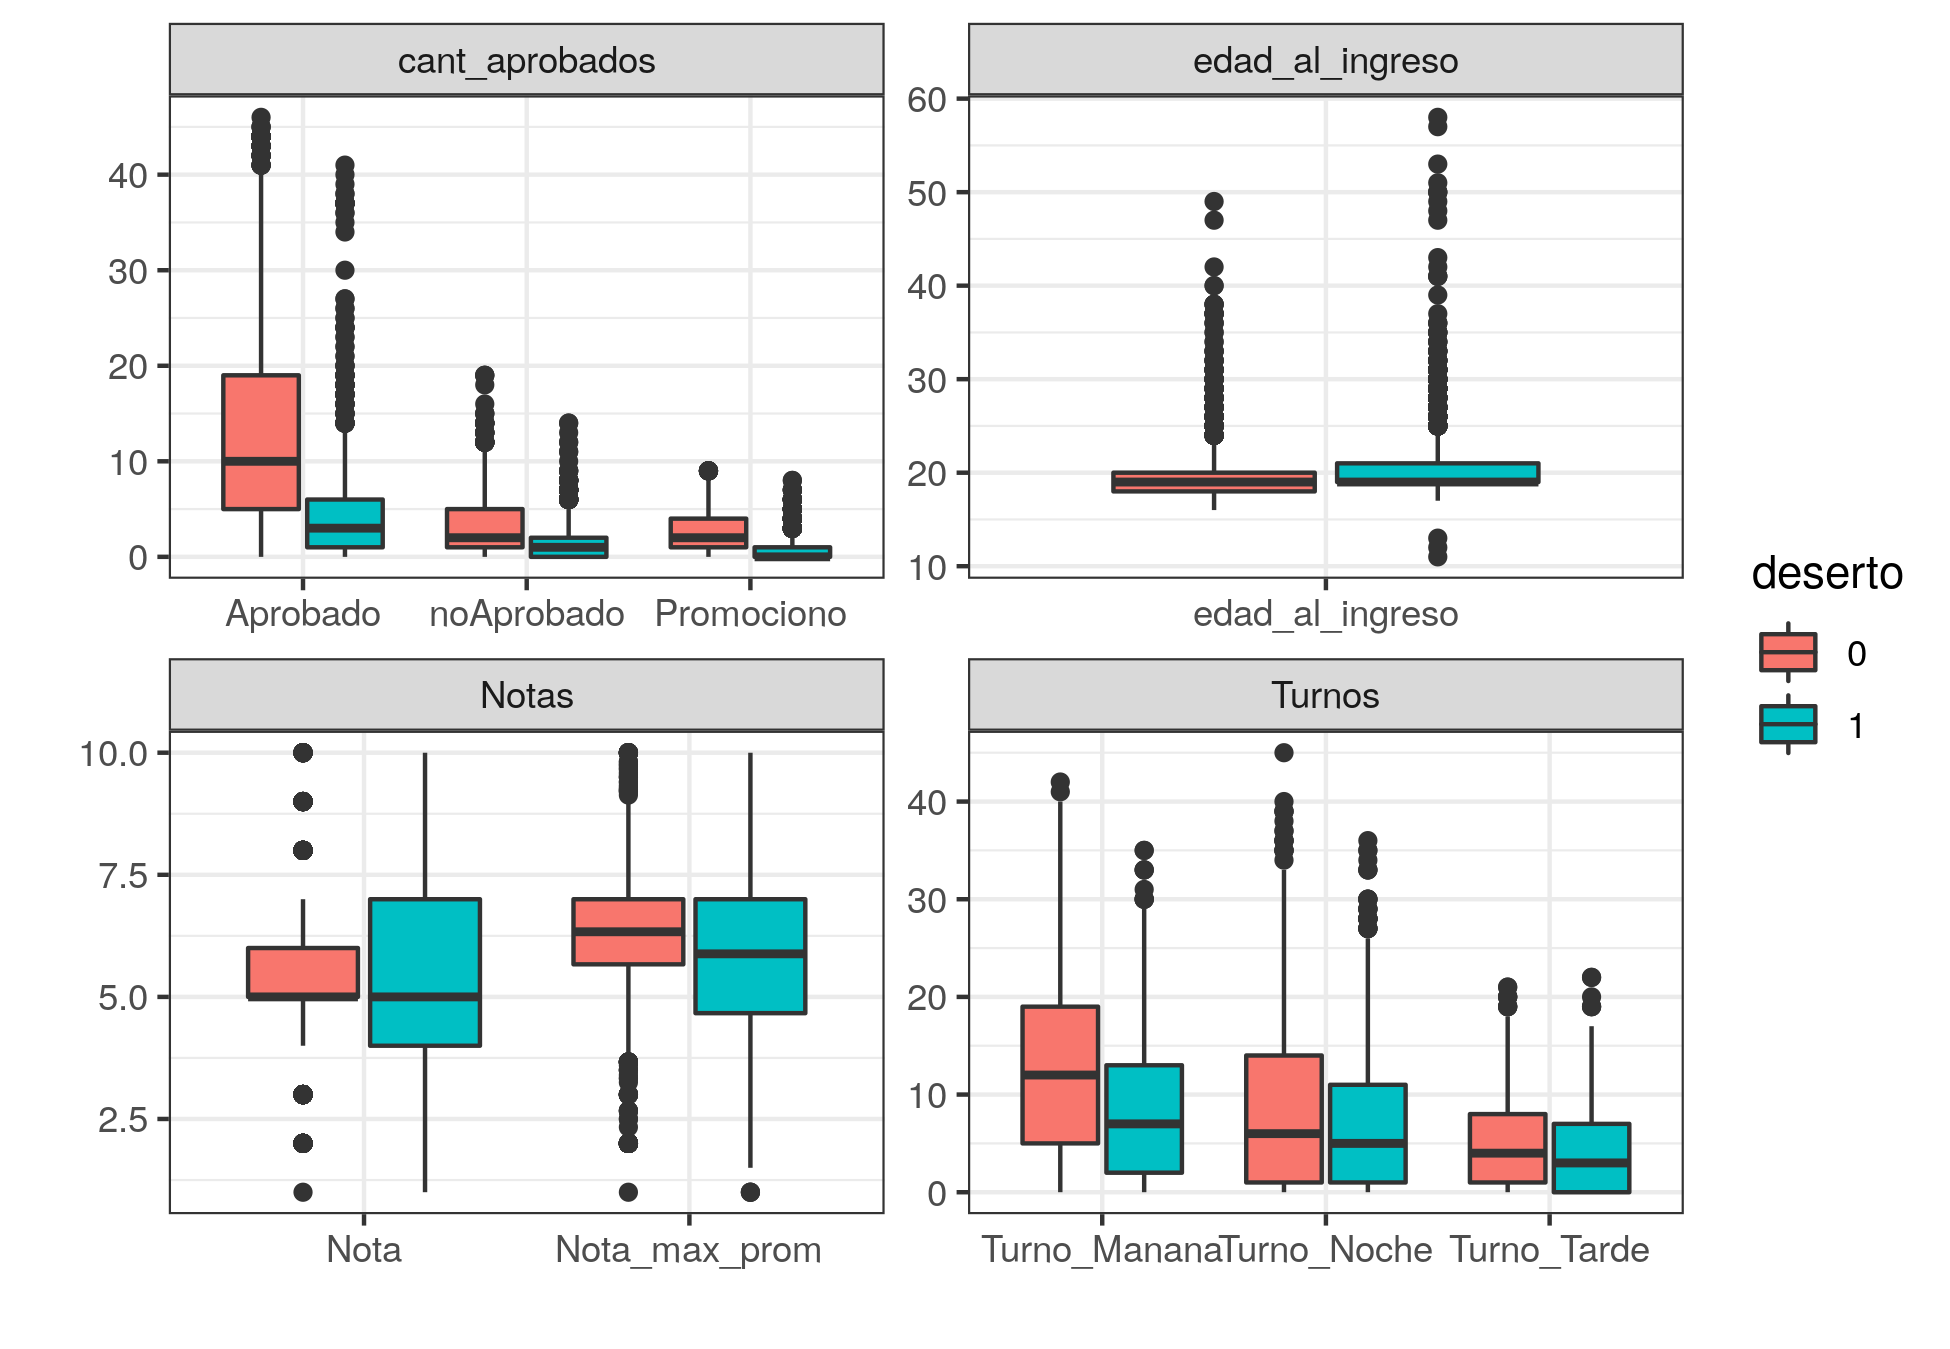
\includegraphics[width=0.9\textwidth]{imagenes/imagenes/gg_explo_tablon_grupo.png}
	%\includegraphics[width=0.25\textwidth]{mesh}
	\caption{Análisis Univariado por grupos}
	\label{fig:tablon_boxplot_grupo}
\end{figure}

\begin{figure}[!htb]
	\centering
	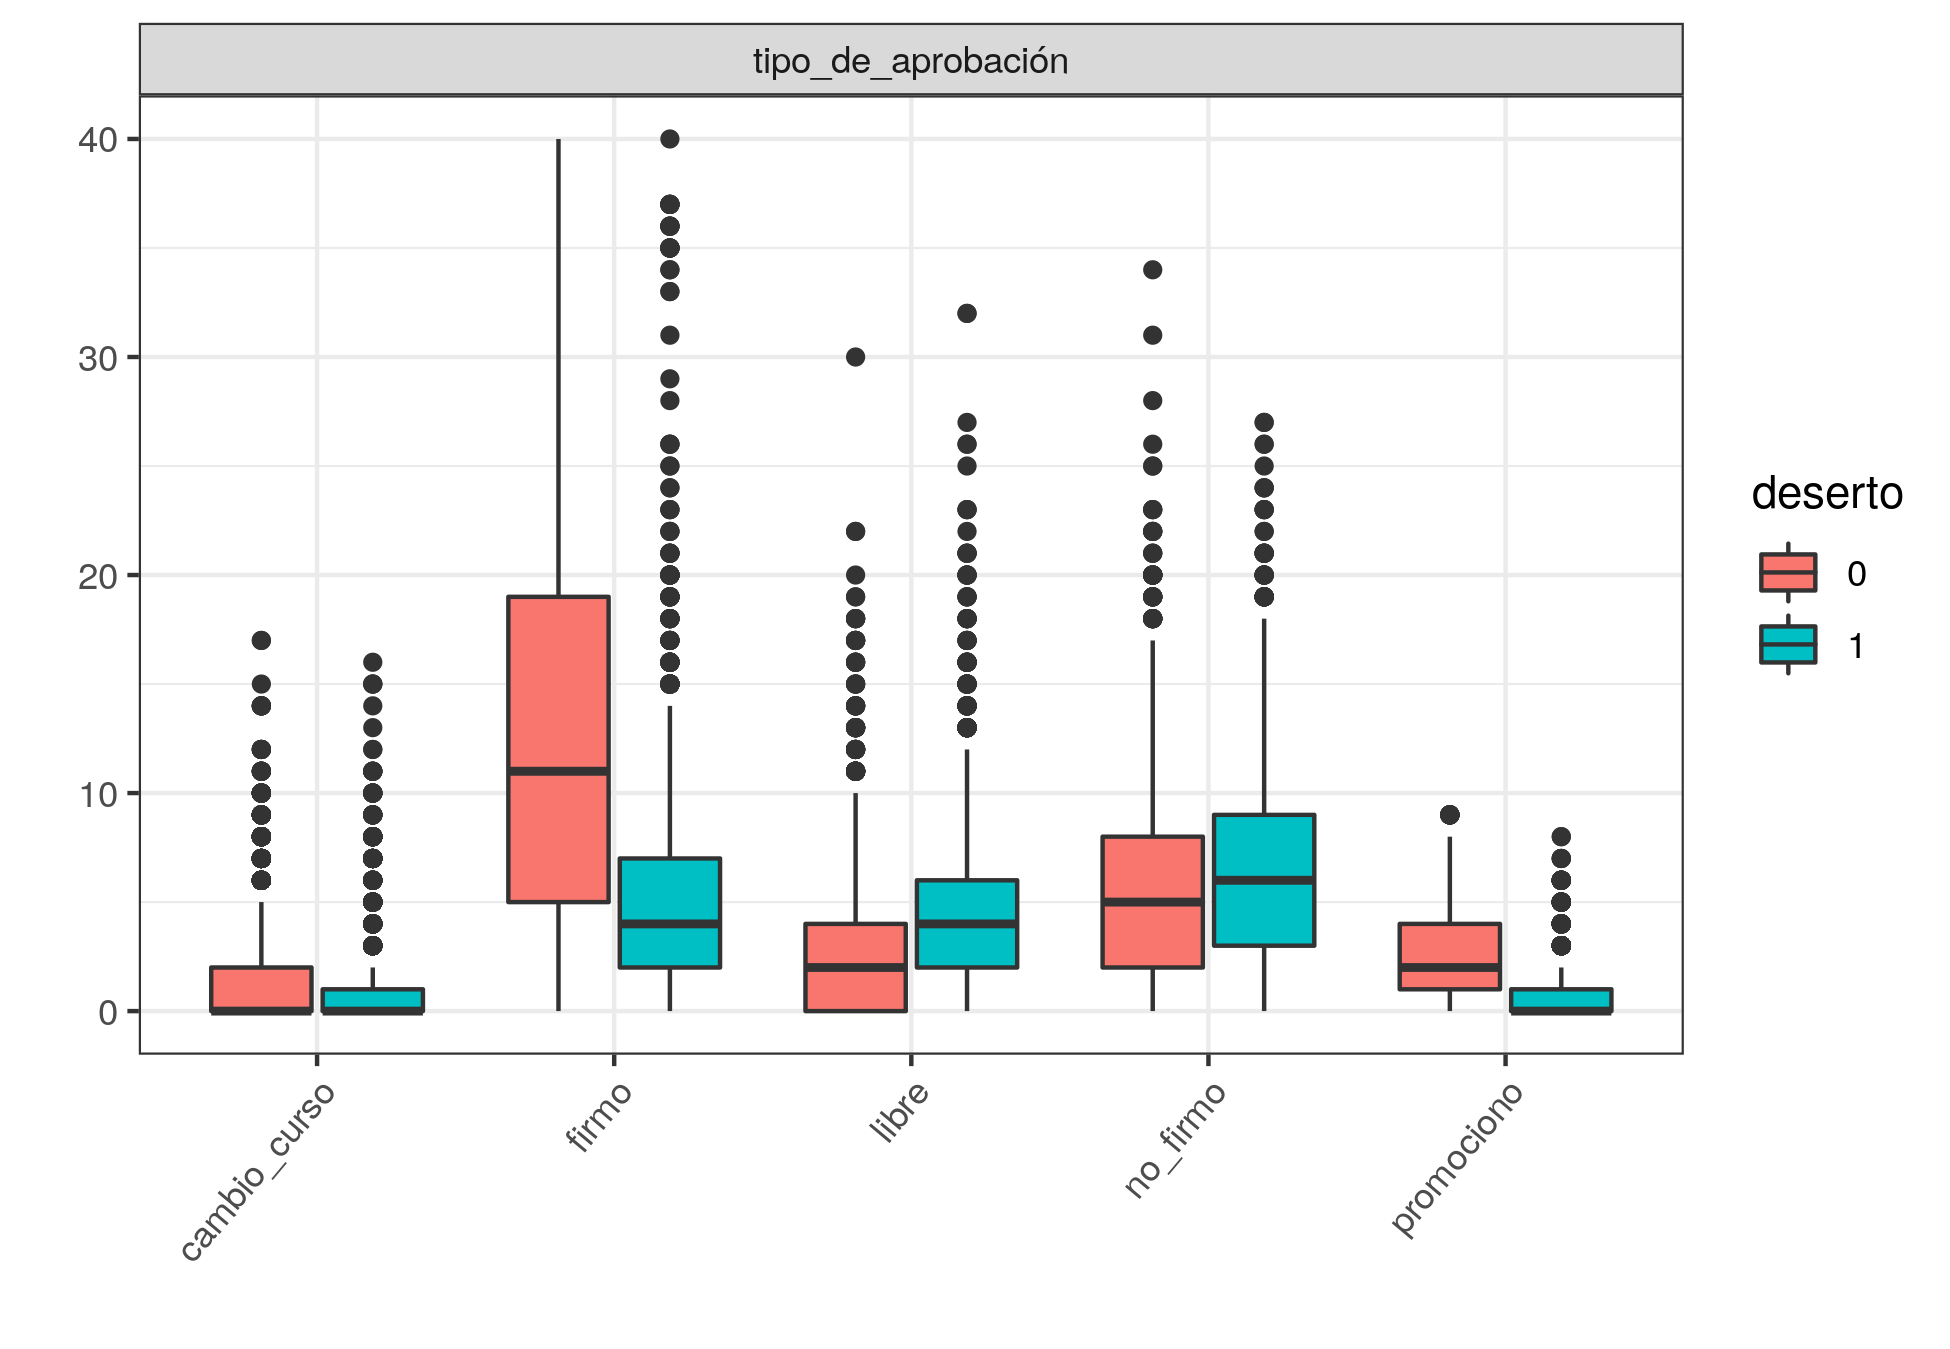
\includegraphics[width=0.9\textwidth]{imagenes/imagenes/gg_explo_tablon_tipo_aprob.png}
	%\includegraphics[width=0.25\textwidth]{mesh}
	\caption{Análisis Univariado por Tipo de Aprobación}
	\label{fig:tablon_boxplot_tipoAprobacion}
\end{figure}

\begin{figure}[!htb]
	\centering
	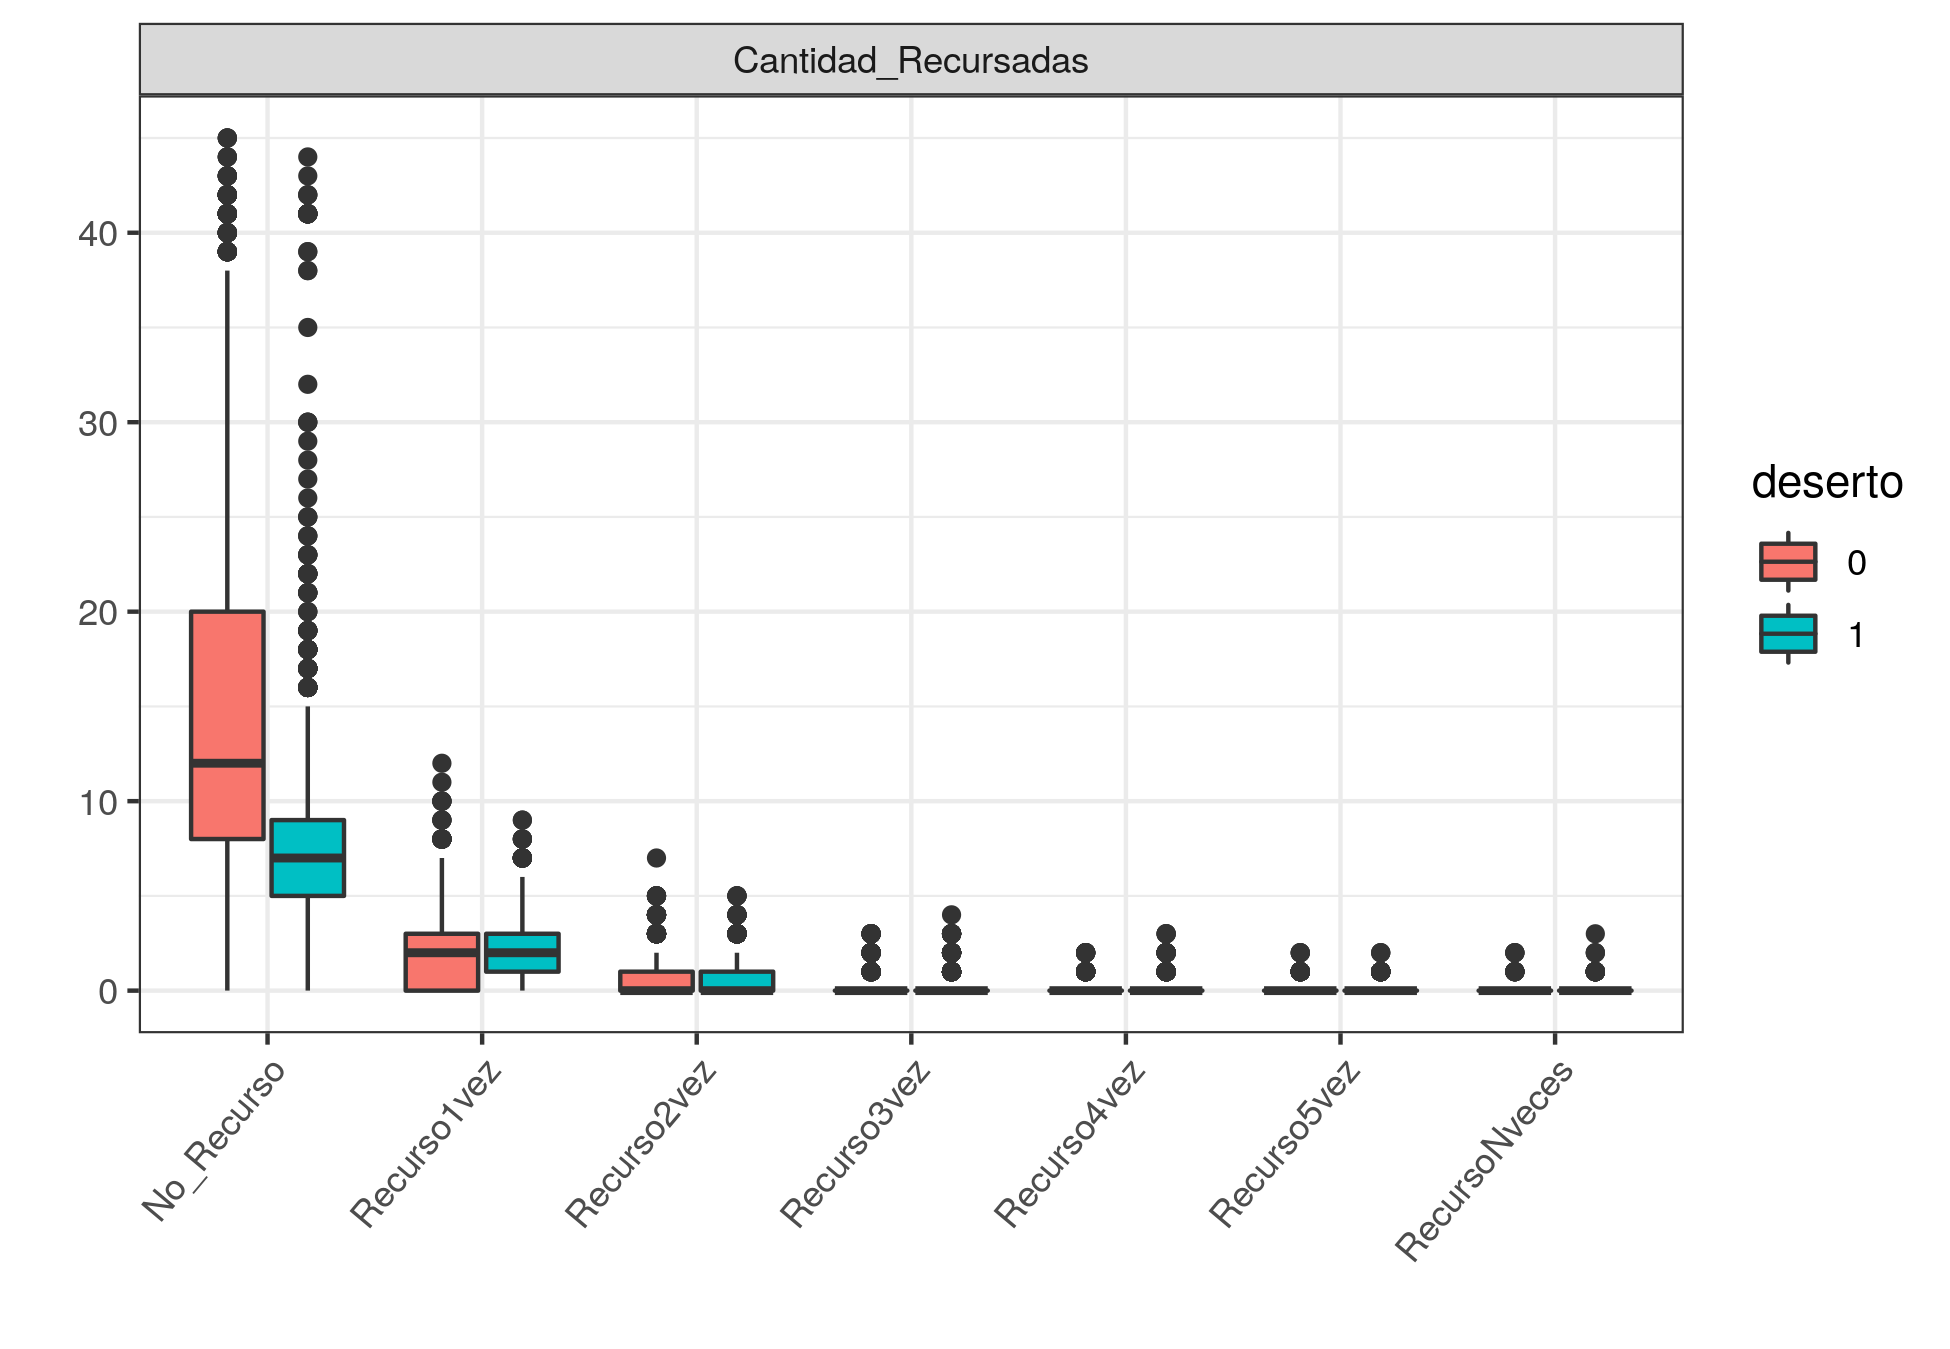
\includegraphics[width=0.9\textwidth]{imagenes/imagenes/gg_explo_tablon_tipo_recur.png}
	%\includegraphics[width=0.25\textwidth]{mesh}
	\caption{Análisis Univariado por tipo de resursada}
	\label{fig:tablon_boxplot_tipoRecursada}
\end{figure}

%\clearpage
\FloatBarrier

\hypertarget{observaciones}{%
	\paragraph{\textbf{\underline{Observaciones}}}\label{observaciones}}

De las tablas y gráficos anteriores podemos extraer la siguiente
información:

\begin{itemize}
	\item
	El dataset se encuentra balanceado. 43.88 \% de los alumnos del
	dataset desertó mientras que el 56.12 \% sigue en carrera.
	\item
	La variable \textbf{EsTecnico} tiene un 13.32\% de datos nulos.
	Dependiendo el método que se use podrá tolerarse o no. En los casos
	que no se pueda tolerar, se tendrá que imputar algún valor o se podrá
	optar por descartar la variable.
	\item
	El valor mínimo de la variable \textbf{edad\_al\_ingreso} es 11. Un
	valor muy bajo y puede tratarse de un error. Se analizaron la cantidad
	de casos que existen en que esta variable tiene un valor menor a 17,
	que es la mínima edad que podría entrar un estudiante a la universidad
	respetando todos los ciclos lectivos sin adelantar ninguno de las
	etapas de estudio anteriores, y dicho valor es de 4 observaciones. Las
	cuales representan una cantidad insignificante respecto del total de
	observaciones 4558 (0.06\%). Por lo tanto al no poder verificarlo por
	el momento se decide dejarlo.
\end{itemize}

\hypertarget{correlaciuxf3n-entre-todas-las-variables}{%
	\paragraph{\underline{\textbf{Correlación entre todas las variables}}}\label{correlaciuxf3n-entre-todas-las-variables}}

%\includegraphics{Analisis_tablon_baseline_2009_files/figure-latex/unnamed-chunk-15-1.pdf}

\begin{figure}[!htb]
	\centering
	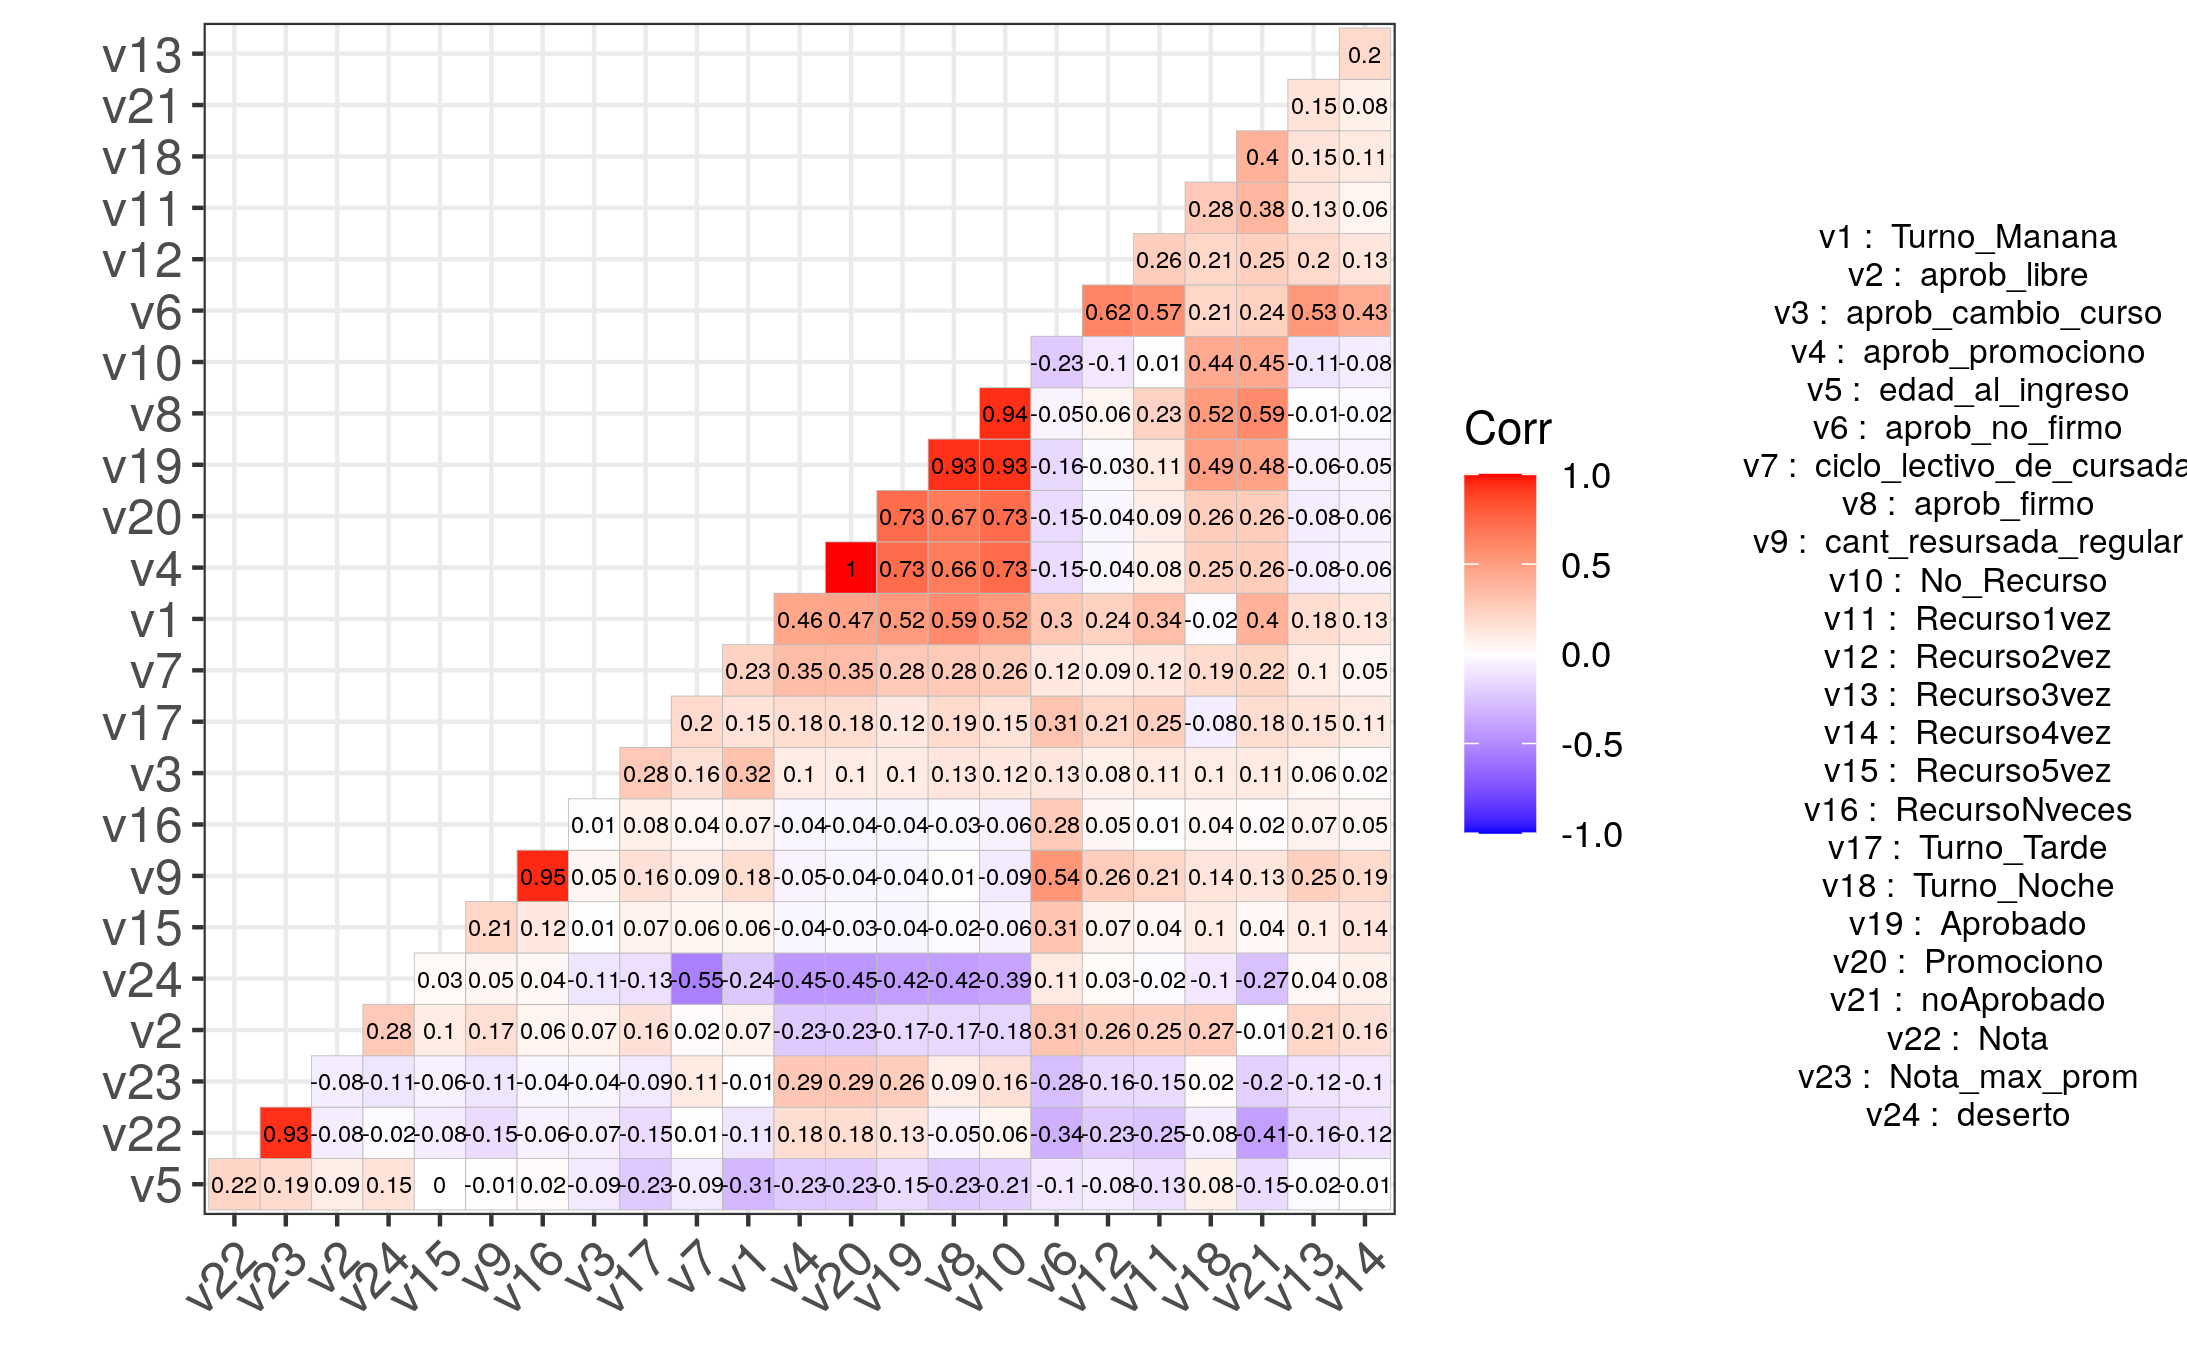
\includegraphics[width=0.98\textwidth]{imagenes/imagenes/gg_corr_todas_variables_leyenda.png}
	%\includegraphics[width=0.25\textwidth]{mesh}
	\caption{Análisis Univariado por tipo de resursada}
	\label{fig:tablon_correlacion}
\end{figure}

\hypertarget{correlaciuxf3n-entre-las-variables-y-la-clase}{%
	\paragraph{\underline{Correlación entre las variables y la clase}}\label{correlaciuxf3n-entre-las-variables-y-la-clase}}

Si bien la clase es categórica y la mayoría de las variables son
numéricas, podemos convertir la clase en númerica convirtiendo los casos
positivos en 1 y los negativos en 0. De esta forma podemos analizar por
el coeficiente de correlación si es que existen variables predictoras
que sigan o se acerquen al comportamiento de la clase. Como veremos en
la sigueinte tabla, no hay una relación muy directa entre cada variable
individual con la clase convertida en numérica.

\begin{table}[!h]
	
	\caption{\label{tab:tablon_correl_clase}Correlacion con la clase}
	\centering
	\begin{tabular}[t]{llr}
		\toprule
		\rowcolor{black}  \multicolumn{1}{c}{\textcolor{white}{\textbf{nombrefila}}} & \multicolumn{1}{c}{\textcolor{white}{\textbf{nombrecolumna}}} & \multicolumn{1}{c}{\textcolor{white}{\textbf{correl}}}\\
		\midrule
		\rowcolor{gray!6}  deserto & ciclo\_lectivo\_de\_cursada & -0.55\\
		deserto & tipo\_de\_aprobacion\_promociono & -0.45\\
		\rowcolor{gray!6}  deserto & Promociono & -0.45\\
		deserto & tipo\_de\_aprobacion\_firmo & -0.42\\
		\rowcolor{gray!6}  deserto & Aprobado & -0.42\\
		\addlinespace
		deserto & cant\_recursada\_regular\_No\_Recurso & -0.39\\
		\rowcolor{gray!6}  deserto & tipo\_de\_aprobacion\_libre & 0.28\\
		deserto & noAprobado & -0.27\\
		\rowcolor{gray!6}  deserto & Turno\_Manana & -0.24\\
		deserto & edad\_al\_ingreso & 0.15\\
		\addlinespace
		\rowcolor{gray!6}  deserto & Turno\_Tarde & -0.13\\
		deserto & tipo\_de\_aprobacion\_no\_firmo & 0.11\\
		\rowcolor{gray!6}  deserto & tipo\_de\_aprobacion\_cambio\_curso & -0.11\\
		deserto & Nota\_max\_prom & -0.11\\
		\rowcolor{gray!6}  deserto & Turno\_Noche & -0.10\\
		\addlinespace
		deserto & cant\_recursada\_regular\_Recurso4vez & 0.08\\
		\rowcolor{gray!6}  deserto & cant\_resursada\_regular & 0.05\\
		deserto & cant\_recursada\_regular\_Recurso3vez & 0.04\\
		\rowcolor{gray!6}  deserto & cant\_recursada\_regular\_RecursoNveces & 0.04\\
		deserto & cant\_recursada\_regular\_Recurso5vez & 0.03\\
		\addlinespace
		\rowcolor{gray!6}  deserto & cant\_recursada\_regular\_Recurso2vez & 0.03\\
		deserto & Nota & -0.02\\
		\rowcolor{gray!6}  deserto & cant\_recursada\_regular\_Recurso1vez & -0.02\\
		\bottomrule
	\end{tabular}
\end{table}



\subsubsection{\textbf{Análisis de Variables Importantes}}\label{analisis-var_importantes}

Incluir un exceso de variables en el modelo suele traer aparejado una disminución de la capacidad predictiva de un modelo cuando se expone a nuevos datos (overfitting). \\
Se realizan múltiples evaluaciones de modelos de RandomForest con bootstrapping generados mediante incorporación y eliminación de predictores con la finalidad de identificar la combinación óptima. Este análisis de realiza únicamente con el datset de train para que los valores de test no influyan en este procedimiento.\\

En la tabla \ref{tab:top_10_rfe_accuracy} se detallan los mejores 10 modelos obtenidos a partir de toda la combinación posibles. Puede observarse que el mejor modelo a juzgar por la métrica Accuracy es el que se entrenó solamente con 10 predictores de los 24 que cuenta el datset completo. Dichos predictores son: 
``ciclo\_lectivo\_de\_cursada",``tipo\_de\_aprobacion\_libre", ``Turno\_Noche", ``tipo\_de\_aprobacion\_no\_firmo", ``Aprobado", ``Turno\_Tarde", ``Nota\_max\_prom", ``tipo\_de\_aprobacion\_firmo", ``Turno\_Manana" y ``cant\_resursada\_regular".\\

Asimismo, en la figura \ref{fig:rfe_evolucion_accuracy} se puede observar la evolución de la métrica accuracy en función de la cantidad de variables que toma el modelo. La dispersión en este caso está asociado a los distintos valores de accuracy que tiene cada modelo ejecutado en cross validation como así también está contemplado todas las combinaciones de variables posibles con la cantidad que marca el eje x.\\
Además de que al usar menos variables se necesita menos poder de computo, es más fácil la interpretación que se podrá hacer y tendremos una menor dispersión final.

\begin{table}[!h]
	
	\caption{\label{tab:top_10_rfe_accuracy}Top 10 Modelos con cantidad de variables seleccionadas según Accuracy}
	\centering
	\begin{tabular}[t]{rrr}
		\toprule
		\rowcolor{black}  \multicolumn{1}{c}{\textcolor{white}{\textbf{Variables}}} & \multicolumn{1}{c}{\textcolor{white}{\textbf{media\_accuracy}}} & \multicolumn{1}{c}{\textcolor{white}{\textbf{media\_kappa}}}\\
		\midrule
		\rowcolor{gray!6}  10 & 0.8388631 & 0.6690887\\
		18 & 0.8385668 & 0.6687514\\
		\rowcolor{gray!6}  11 & 0.8381883 & 0.6678640\\
		19 & 0.8381476 & 0.6679149\\
		\rowcolor{gray!6}  17 & 0.8380654 & 0.6677621\\
		\addlinespace
		9 & 0.8377655 & 0.6670357\\
		\rowcolor{gray!6}  23 & 0.8368520 & 0.6655250\\
		20 & 0.8360972 & 0.6636373\\
		\rowcolor{gray!6}  15 & 0.8360919 & 0.6637290\\
		22 & 0.8355010 & 0.6625480\\
		\bottomrule
	\end{tabular}
\end{table}

\begin{figure}[!htb]
	\centering
	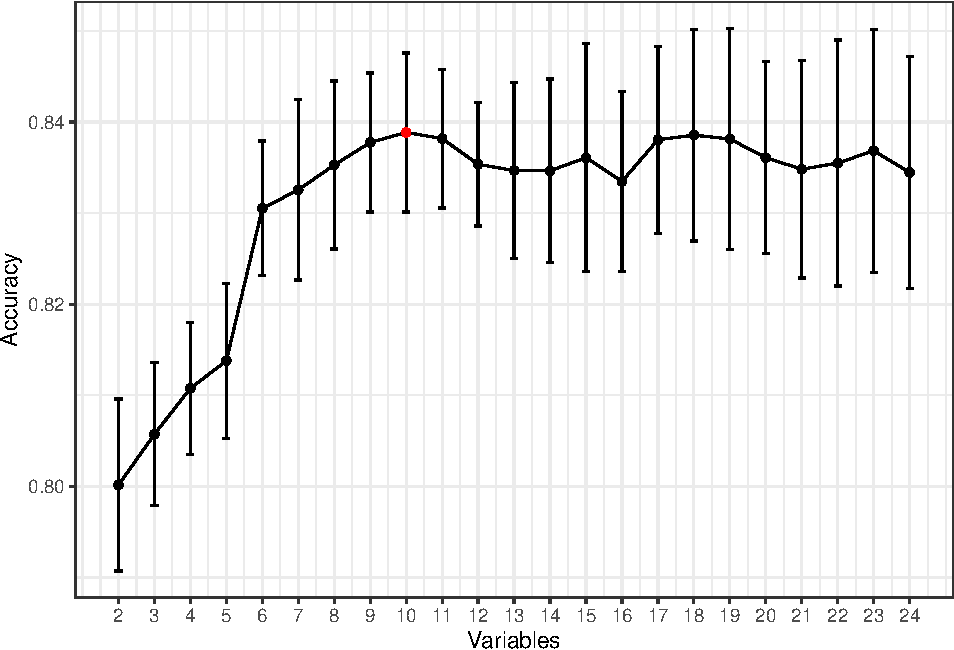
\includegraphics[width=0.9\textwidth]{imagenes/variables/rfe_evolucion_accuracy-1.pdf}
	%\includegraphics[width=0.25\textwidth]{mesh}
	\caption{Evolución de la métrica Accuracy en función de la cantidad de variables usadas por el modelo}
	\label{fig:rfe_evolucion_accuracy}
\end{figure}

\paragraph{\underline{influencia de variables:}}
Tras ajustar cada uno de estos modelos, se recalcula la influencia de cada variable. De esta forma, para cada tamaño de modelo, se obtiene un ranking de la importancia promedio de las variables. Los resultados se pueden observar en \ref{tab:tf_rfe_influencia_variables} y \ref{fig:rfe_influencia_var} donde existe una variable que claramente influye mucho más en los resultados en comparación con los otros predictores.

\begin{table}[!h]
	
	\caption{\label{tab:tf_rfe_influencia_variables}Influencia de variables en el resultado}
	\centering
	\begin{tabular}[t]{lrr}
		\toprule
		\rowcolor{black}  \multicolumn{1}{c}{\textcolor{white}{\textbf{var}}} & \multicolumn{1}{c}{\textcolor{white}{\textbf{media\_influencia}}} & \multicolumn{1}{c}{\textcolor{white}{\textbf{sd\_influencia}}}\\
		\midrule
		\rowcolor{gray!6}  ciclo\_lectivo\_de\_cursada & 89.84 & 2.97\\
		tipo\_de\_aprobacion\_libre & 46.34 & 2.26\\
		\rowcolor{gray!6}  Turno\_Noche & 38.08 & 1.72\\
		tipo\_de\_aprobacion\_no\_firmo & 38.05 & 1.54\\
		\rowcolor{gray!6}  Aprobado & 35.81 & 1.13\\
		\addlinespace
		Turno\_Tarde & 35.67 & 1.50\\
		\rowcolor{gray!6}  tipo\_de\_aprobacion\_firmo & 35.29 & 0.69\\
		Nota\_max\_prom & 35.14 & 2.40\\
		\rowcolor{gray!6}  Turno\_Manana & 34.31 & 1.60\\
		cant\_resursada\_regular & 32.25 & 1.19\\
		\addlinespace
		\rowcolor{gray!6}  edad\_al\_ingreso & 31.90 & 0.10\\
		\bottomrule
	\end{tabular}
\end{table}

\FloatBarrier

\begin{figure}[!htb]
	\centering
	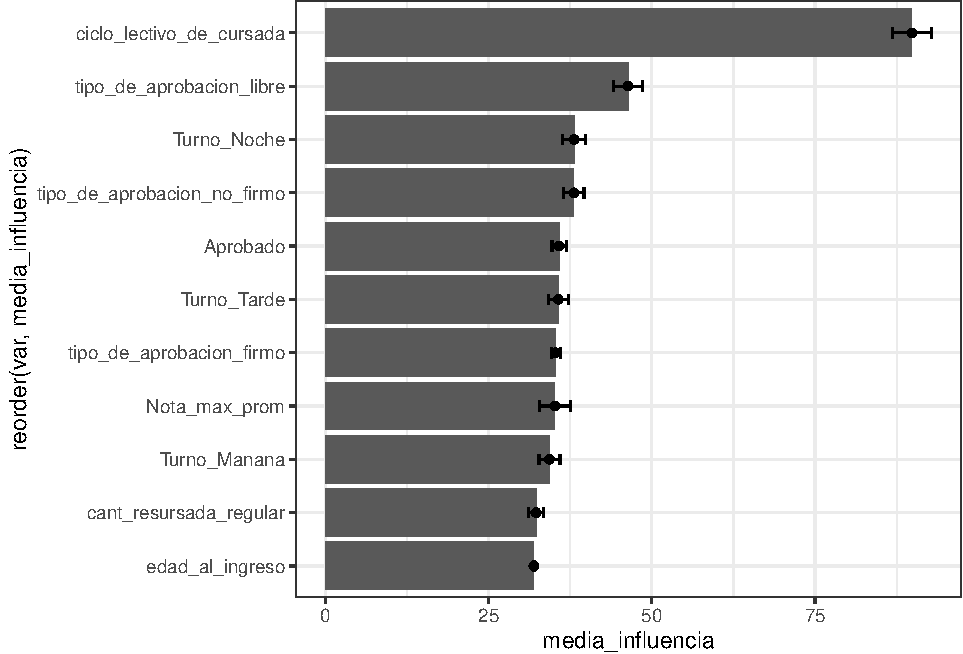
\includegraphics[width=0.9\textwidth]{imagenes/variables/influencia_de_variables-1.pdf}
	%\includegraphics[width=0.25\textwidth]{mesh}
	\caption{Influencia de las variables mas importances sobre el resultado}
	\label{fig:rfe_influencia_var}
\end{figure}

%\clearpage
\FloatBarrier


\subsubsection{\textbf{Análisis de Variables Importantes:} Dataset sin Variable ``ciclo\_lectivo\_de\_cursada"}\label{analisis-var_importantes-2}

De acuerdo al análisis de Variables anterior, se decide eliminar la variable mas influyente en el resultado (``ciclo\_lectivo\_de\_cursada'') y analizar el dataset resultante. Esto se realiza para verificar que aún sin esa información es posible armar buenos modelos predictivos.

Se utiliza la misma técnica anterior de múltiples evaluaciones con  modelos de RandomForest con bootstrapping generados mediante incorporación y eliminación de predictores con la finalidad de identificar la combinación óptima. Este análisis de realiza unicamente con el datset de train para que los valores de test no influyan en este procedimiento.\\

En la tabla \ref{tab:top_10_rfe_accuracy_datasetAlternativa2} se detallan los mejores 10 modelos obtenidos a partir de todas las combinaciones posibles. El mejor modelo a juzgar por la métrica Accuracy es el que se entrena con todos los predictores disponibles.

Asimismo, en la figura \ref{fig:rfe_evolucion_accuracy_datasetAlternativa2} se puede observar la evolución de la métrica accuracy en función de la cantidad de variables que toma el modelo. La dispersión en este caso está asociado a los distintos valores de accuracy que tiene cada modelo ejecutado en cross validation como así también está contemplado todas las combinaciones de variables posibles con la cantidad que marca el eje x.\\
Se puede observar que desde que la cantidad de variables es 15, el Accuracy obtenido es un valor muy próximo al máximo que se consigue con 23 variables. Por lo que, si se opta por este dataset y se lo quisiera explicar quizas sería mas sencillo con menos variables aunque sigue siendo una cantidad considerablemente alta para extraer conclusiones sencillas y dependerá mucho de la interacción entre ellas.\\


\begin{table}[!h]
	
	\caption{\label{tab:top_10_rfe_accuracy_datasetAlternativa2}Top 10 Modelos con cantidad de variables seleccionadas según Accuracy}
	\centering
	\begin{tabular}[t]{rrr}
		\toprule
		\rowcolor{black}  \multicolumn{1}{c}{\textcolor{white}{\textbf{Variables}}} & \multicolumn{1}{c}{\textcolor{white}{\textbf{media\_accuracy}}} & \multicolumn{1}{c}{\textcolor{white}{\textbf{media\_kappa}}}\\
		\midrule
		\rowcolor{gray!6}  23 & 0.7747542 & 0.5421768\\
		20 & 0.7736578 & 0.5399892\\
		\rowcolor{gray!6}  18 & 0.7732554 & 0.5390105\\
		15 & 0.7720421 & 0.5368054\\
		\rowcolor{gray!6}  21 & 0.7720411 & 0.5363012\\
		\addlinespace
		22 & 0.7714524 & 0.5355353\\
		\rowcolor{gray!6}  17 & 0.7710945 & 0.5346718\\
		16 & 0.7710278 & 0.5348438\\
		\rowcolor{gray!6}  19 & 0.7707567 & 0.5340365\\
		14 & 0.7673518 & 0.5279523\\
		\bottomrule
	\end{tabular}
\end{table}

\begin{figure}[!htb]
	\centering
	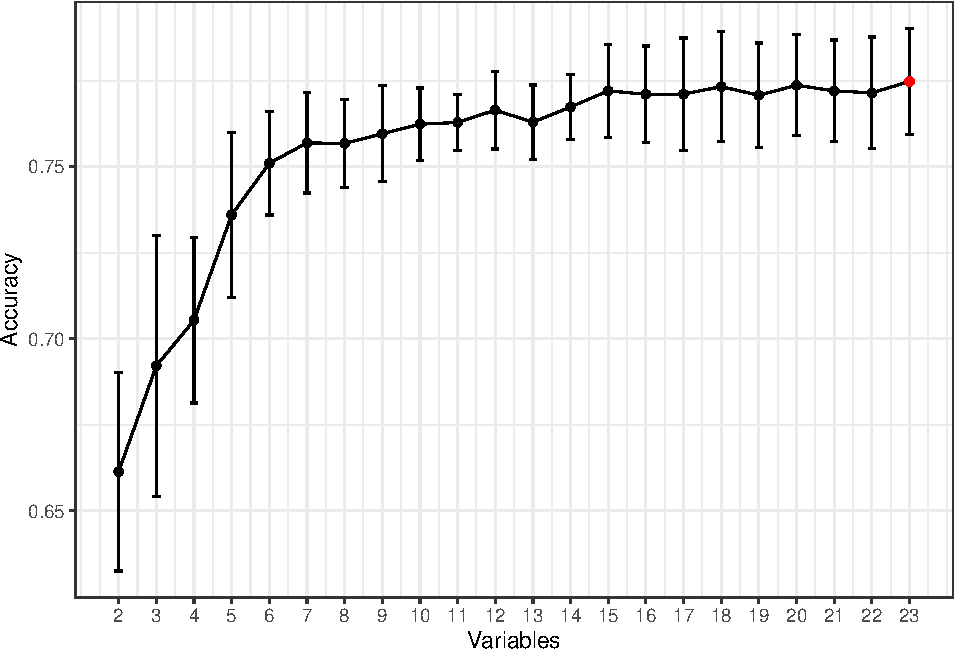
\includegraphics[width=0.9\textwidth]{imagenes/variables/rfe_evolucion_accuracy-1_alternativa2.pdf}
	%\includegraphics[width=0.25\textwidth]{mesh}
	\caption{Evolución de la Métrica Accuracy en función de la cantidad de variables usadas por el modelo}
	\label{fig:rfe_evolucion_accuracy_datasetAlternativa2}
\end{figure}

\paragraph{\underline{influencia de variables}}
Tras ajustar cada modelo, se recalcula la influencia de cada variable.
De esta forma, para cada tamaño de modelo, se obtiene un ranking de la
importancia promedio de las variables. Los resultados se pueden observar en \ref{tab:tf_rfe_influencia_variables_23} y \ref{fig:rfe_influencia_var_dsalternativa2}. Se puede observar que la influencia sobre el resultado final ahora es mas equitativo entre las variables.


\begin{figure}[!htb]
	\centering
	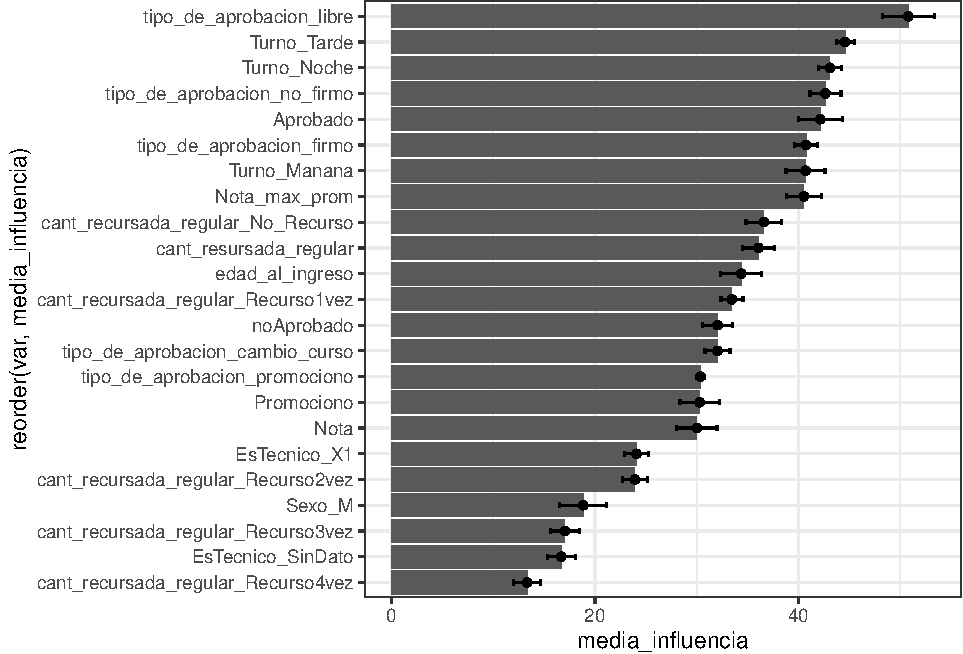
\includegraphics[width=0.9\textwidth]{imagenes/variables/influencia_de_variables_23-1.pdf}
	%\includegraphics[width=0.25\textwidth]{mesh}
	\caption{Influencia de las variables más importantes sobre el resultado}
	\label{fig:rfe_influencia_var_dsalternativa2}
\end{figure}

\FloatBarrier

\begin{table}[!h]
	
	\caption{\label{tab:tf_rfe_influencia_variables_23}Influencia de variables en el resultado}
	\centering
	\begin{tabular}[t]{lrr}
		\toprule
		\rowcolor{black}  \multicolumn{1}{c}{\textcolor{white}{\textbf{var}}} & \multicolumn{1}{c}{\textcolor{white}{\textbf{media\_influencia}}} & \multicolumn{1}{c}{\textcolor{white}{\textbf{sd\_influencia}}}\\
		\midrule
		\rowcolor{gray!6}  tipo\_de\_aprobacion\_libre & 50.79 & 2.55\\
		Turno\_Tarde & 44.60 & 0.89\\
		\rowcolor{gray!6}  Turno\_Noche & 43.09 & 1.15\\
		tipo\_de\_aprobacion\_no\_firmo & 42.65 & 1.52\\
		\rowcolor{gray!6}  Aprobado & 42.15 & 2.14\\
		\addlinespace
		tipo\_de\_aprobacion\_firmo & 40.75 & 1.11\\
		\rowcolor{gray!6}  Turno\_Manana & 40.69 & 1.91\\
		Nota\_max\_prom & 40.54 & 1.72\\
		\rowcolor{gray!6}  cant\_recursada\_regular\_No\_Recurso & 36.59 & 1.76\\
		cant\_resursada\_regular & 36.06 & 1.60\\
		\addlinespace
		\rowcolor{gray!6}  edad\_al\_ingreso & 34.36 & 2.01\\
		cant\_recursada\_regular\_Recurso1vez & 33.46 & 1.08\\
		\rowcolor{gray!6}  noAprobado & 32.05 & 1.49\\
		tipo\_de\_aprobacion\_cambio\_curso & 32.04 & 1.22\\
		\rowcolor{gray!6}  tipo\_de\_aprobacion\_promociono & 30.37 & 0.42\\
		\addlinespace
		Promociono & 30.31 & 1.94\\
		\rowcolor{gray!6}  Nota & 30.01 & 1.97\\
		EsTecnico\_X1 & 24.08 & 1.19\\
		\rowcolor{gray!6}  cant\_recursada\_regular\_Recurso2vez & 23.94 & 1.22\\
		Sexo\_M & 18.85 & 2.29\\
		\addlinespace
		\rowcolor{gray!6}  cant\_recursada\_regular\_Recurso3vez & 17.05 & 1.40\\
		EsTecnico\_SinDato & 16.70 & 1.38\\
		\rowcolor{gray!6}  cant\_recursada\_regular\_Recurso4vez & 13.33 & 1.30\\
		\bottomrule
	\end{tabular}
\end{table}







%-------------------------------------------------%
\section{Formateo de los datos}
%-------------------------------------------------%
\comentarioinvisible{en esta seccion hace referencia si hayq eu formatear los campos de alguna forma dependiendo el modelo que se utilice.}

\todorevisar{ como son varios modelos los qu se van a aplicar y quizas cada uno requiere formatos distintos, quizas es mejor hacerlo directamente con los modelos.}

%%%% MODELADO
%-------------------------------------------------%
\chapter{Modelado}
%-------------------------------------------------%
%-------------------------------------------------%
\section{Seleccionar la técnica de modelado}
%-------------------------------------------------%
Si bien el dataset de trabajo contiene una clase, se utilizarán técnicas supervisadas y no supervisadas.

Las técnicas a emplear son:
\begin{itemize}
	\item Clusters
	\item Árboles de decisión
	\item RandomForest
	\item Gradient Boosting
	\item Support Vector Machine (SVM)
	\item Regresión logística
	\item modelos de modelos (se refiere a que se utilizarán mas de un tipo de técnica que interactuarán y formarán nuevos modelos)
\end{itemize}


En este documento habrá una sección dedicada a cada modelo particular empleado. En dicha sección se explicará brevemente porque la elección de dicha técnica y cual es su aplicación o finalidad para la cual se emplea.
%-------------------------------------------------%
\section{Generar el diseño de prueba}
%-------------------------------------------------%

En esta sección se especifican los conjuntos de datos usados en los diferentes modelos.

Los \textbf{modelos no supervisados} utilizarán todo el tablón o mejor expresado, el dataset integrado en su totalidad. Es decir \textit{"baseline\_2009.csv"}. \ref{tablon_integrado} \\

Los \textbf{modelos supervisados} utilizarán el tablón mencionado anteriormente pero dividido en 70\% para train y 30\% para test. A su vez, el conjunto de train puede ser subdividio en train y validation si el modelo lo utiliza.
Los nombres de los conjuntos de entrenamiento y testeo son \textit{"baseline\_2009\_train.csv"} y \textit{"baseline\_2009\_test.csv"} respectivamente.
La generación de dichos conjuntos se realiza en la siguiente sección \ref{dataset_train_test}.

%-------------------------------------------------%
\subsection{Crear conjuntos de entrenamiento y de prueba}\label{dataset_train_test}
%-------------------------------------------------%

Los conjuntos de train y test se dividen de manera estratificada con la clase y de manera aleatoria con las observaciones. El conjunto train a su vez es subdividido en la etapa de creación de modelos en en train y validation para que en conjunto con técnicas como cross-validation para disminuir o evitar el sobreajuste durante el entrenamiento.\\

La proporción de ambos datasets ha quedado en 56\% de no desertores y 44\% de desertores.



%-------------------------------------------------%
\subsubsection{Otros Datasets}
%-------------------------------------------------%

\paragraph{Reducción de Dimensión: Análisis de Componentes Principales}\label{anuxe1lisis-de-componentes-principales}

Se aplica la técnica de Componentes Principales para reducir la cantidad de variables predictoras pero que a su vez sigan mantengan un gran porcentaje de la variabilidad total.\\
El resultado puede observarse en \ref{fig:pca_varexp_comp}, \ref{tab:loadings_pca_tablon} y \ref{fig:pca_biplot}. Los mismo indican que si bien se puede reducir la cantidad de variables
predictoras y mantener una alta variabilidad de la información
explicada, los diagramas de biplot en este caso no nos servirían de
mucha ayuda ya que en las primeras 2 componentes solo se explica el 41\%
y en las primeras 4 componentes solo el 56\%. Además, los loadings de
dichas componentes no tienen una clara identificación de lo que significan las proyecciónes, por lo que sería complicado explicar el modelo que se quiera desarrollar según estas nuevas variables.

\begin{figure}[!htb]
	\centering
	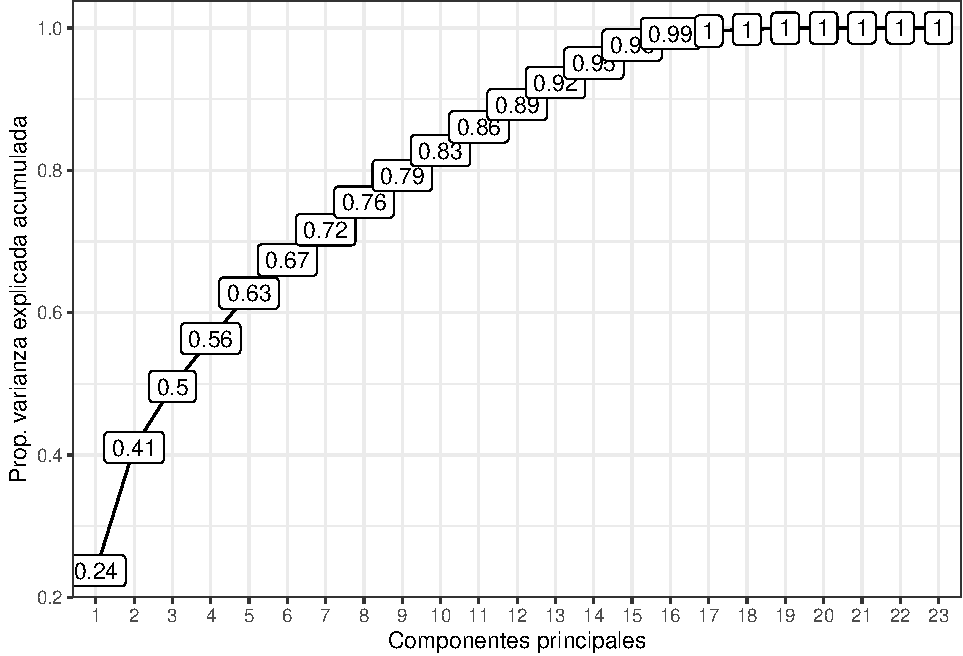
\includegraphics{imagenes/reduccion_dimension/unnamed-chunk-7-1.pdf}
	%\includegraphics[width=0.25\textwidth]{mesh}
	\caption{PCA: Variabilidad explicada VS Componentes}
	\label{fig:pca_varexp_comp}
\end{figure}



\begin{table}[!h]
	
	\caption{\label{tab:loadings_pca_tablon}Loadings de PCA en Tablon}
	\centering
	\begin{tabular}[t]{lrrrr}
		\toprule
		\rowcolor{black}  \multicolumn{1}{c}{\textcolor{white}{\textbf{variable}}} & \multicolumn{1}{c}{\textcolor{white}{\textbf{PC1}}} & \multicolumn{1}{c}{\textcolor{white}{\textbf{PC2}}} & \multicolumn{1}{c}{\textcolor{white}{\textbf{PC3}}} & \multicolumn{1}{c}{\textcolor{white}{\textbf{PC4}}}\\
		\midrule
		\rowcolor{gray!6}  Turno\_Manana & 0.2813063 & -0.1375132 & 0.0171629 & 0.0891187\\
		tipo\_de\_aprobacion\_libre & -0.0516192 & -0.2204644 & -0.1151088 & -0.3721061\\
		\rowcolor{gray!6}  tipo\_de\_aprobacion\_cambio\_curso & 0.0985927 & -0.0960438 & 0.0259816 & -0.0003118\\
		tipo\_de\_aprobacion\_promociono & 0.3581733 & 0.1308245 & -0.0808955 & 0.0804953\\
		\rowcolor{gray!6}  edad\_al\_ingreso & -0.1269356 & 0.0733137 & -0.2349852 & -0.2976394\\
		\addlinespace
		tipo\_de\_aprobacion\_no\_firmo & 0.0156176 & -0.4488391 & -0.1126781 & -0.1126948\\
		\rowcolor{gray!6}  ciclo\_lectivo\_de\_cursada & 0.1818683 & -0.0532719 & -0.1144249 & -0.0532596\\
		tipo\_de\_aprobacion\_firmo & 0.3996032 & 0.0206986 & 0.0690403 & -0.0132481\\
		\rowcolor{gray!6}  cant\_resursada\_regular & 0.0227835 & -0.3127946 & -0.4101361 & 0.3674317\\
		cant\_recursada\_regular\_No\_Recurso & 0.3869691 & 0.1219610 & 0.0468956 & 0.0352279\\
		\addlinespace
		\rowcolor{gray!6}  cant\_recursada\_regular\_Recurso1vez & 0.1188652 & -0.2681558 & 0.0654967 & -0.1891977\\
		cant\_recursada\_regular\_Recurso2vez & 0.0451665 & -0.2939066 & -0.0071695 & -0.1971879\\
		\rowcolor{gray!6}  cant\_recursada\_regular\_Recurso3vez & 0.0120116 & -0.2503402 & -0.0867234 & -0.1612458\\
		cant\_recursada\_regular\_Recurso4vez & 0.0044083 & -0.1971933 & -0.0845225 & -0.1281708\\
		\rowcolor{gray!6}  cant\_recursada\_regular\_Recurso5vez & 0.0006389 & -0.1464459 & -0.1411299 & 0.0048529\\
		\addlinespace
		cant\_recursada\_regular\_RecursoNveces & -0.0021967 & -0.1955233 & -0.4257671 & 0.4879239\\
		\rowcolor{gray!6}  Turno\_Tarde & 0.1153361 & -0.1754377 & 0.0127343 & 0.0859205\\
		Turno\_Noche & 0.2032766 & -0.1098708 & -0.0798642 & -0.3755512\\
		\rowcolor{gray!6}  Aprobado & 0.3918783 & 0.1006967 & -0.0242947 & -0.0374767\\
		Promociono & 0.3589365 & 0.1289055 & -0.0812155 & 0.0798013\\
		\addlinespace
		\rowcolor{gray!6}  noAprobado & 0.2504186 & -0.1806504 & 0.2037648 & -0.0519875\\
		Nota & -0.0001346 & 0.3003970 & -0.4732939 & -0.2012817\\
		\rowcolor{gray!6}  Nota\_max\_prom & 0.0688392 & 0.2670847 & -0.4728596 & -0.2279385\\
		\bottomrule
	\end{tabular}
\end{table}

\begin{figure}[!htb]
	\centering
	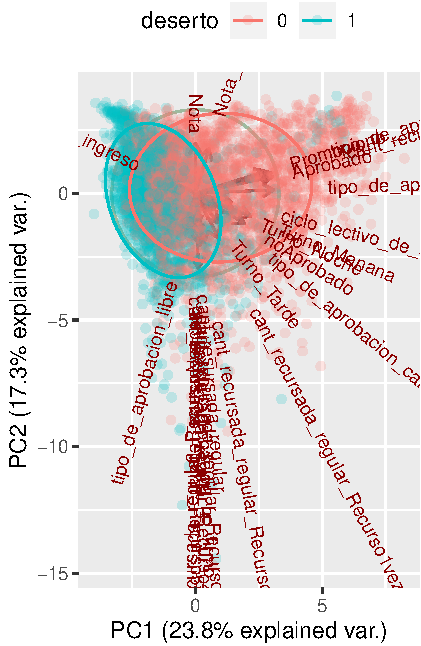
\includegraphics{imagenes/reduccion_dimension/unnamed-chunk-9-1.pdf}
	%\includegraphics[width=0.25\textwidth]{mesh}
	\caption{PCA: biplot PC1 y PC2}
	\label{fig:pca_biplot}
\end{figure}

\paragraph{Reducción de Dimensión: Reducción por t-SNE}\label{reducciuxf3n-por-t-sne}

Al igual que PCA, existen otro algoritmos que pueden realizar reducción
de dimensionalidad. Unos de esos casos es el método no lineal
t-distributed stochastic neighbor embedding (t-SNE), que en ciertos
casos es ventajoso respecto a PCA ya que éste último solo aplica reducción utilizando solamente
combinaciones lineales de las variables originales.\\

Por lo tanto se aplica dicho método de reducción al tablón original y al mismo tiempo se identifican las observaciones según el target real (variable no incluida al hacer la reducción). Cuyos resultados \ref{fig:tsne} indican que si bien no se arman grupos bien definidos,
al identificar cada observación con un color en el gráfico según el
target puede observarse que están mas separadas y hay menos solapamiento entre ellas que con el método PCA. Este resultado puede insinuar que es posible clasificar un gran porcentaje de los casos correctamente a costa quizás de no poder describir o explicar fácilmente como se ha llegado a los resultados.


\begin{figure}[!htb]
	\centering
	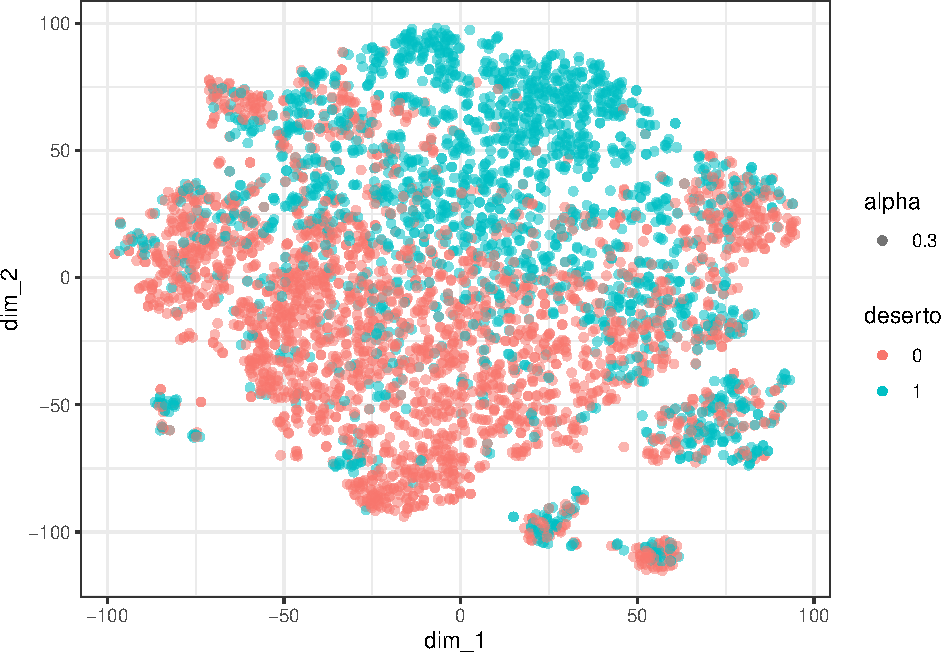
\includegraphics{imagenes/reduccion_dimension/unnamed-chunk-11-1.pdf}
	%\includegraphics[width=0.25\textwidth]{mesh}
	\caption{t-SNE}
	\label{fig:tsne}
\end{figure}

\clearpage




\label{conjunto_datos}
%-------------------------------------------------%
%-------------------------------------------------%
\section{Generación de modelo}\label{generacion_modelos}
%-------------------------------------------------%
%%-------------------------------------------------%
\subsection{Modelo: xxx}
%-------------------------------------------------%

%-------------------------------------------------%
\subsubsection{Determinar parámetros del modelo}
%-------------------------------------------------%
%-------------------------------------------------%
\subsubsection{Modelar}
%-------------------------------------------------%
%-------------------------------------------------%
\subsubsection{Describir el modelo}
%-------------------------------------------------%
%-------------------------------------------------%
\subsection{Modelo: Clusters}
%-------------------------------------------------%

Se utilizarán técnicas de clusters sobre la base del tablón con el objetivo de observar si realmente existen agrupamientos basados en las características que contiene el tablón. Al terminar, se ingresará el clase sobre cada individuo y se analizará la composición de cada agrupamiento si se corresponde con dicho target. \\

\paragraph{\textbf{Criterio:}}

Como son solamente 2 las variables categóricas (EsTecnico y
sexo), en vez de calcular las distancias numéricas por un lado
(euclídea, manhattan, correlación, etc), las distancias categóricas por
otras (SMC, Jaccard, etc) y tratar de transformar esas matrices de
distancias en una nueva matriz unificada con criterios, se decide
transformar los datos categóricos en numéricos aprovechando que ambos
campos tiene solamente 2 valores por lo que estarán en los extremos
tomando una normalización entre 0 y 1. En el caso de las observaciones con valor nulo en la variable EsTecnico, se imputará con el valor
0.5 (mitad entre extremos)

\paragraph{Análisis de tendencia al agrupamiento}

El estadístico de Hopkins sobre el tablón original transformando las 2
variable categóricas en numéricas da 0.8893004. Es un valor cercano a 1
por lo que tiene mucha tendencia a ser clusterizado.

%-------------------------------------------------%
\subsubsection{\textbf{Determinar parámetros del modelo}}
%-------------------------------------------------%

\paragraph{\textbf{Matriz de Distancias de observaciones:}} euclideana

\paragraph{\textbf{Número óptimo de clusters}} \label{estudio-del-numero-optimo-de-clusters}
Para este estudio, se aplicaron 2 técnicas de agrupamiento llamadas kmeans y jerárquico. Se han calculado distintas métricas de agrupamiento y conectividad para determinar cual es el número óptimo de clusters, tomando como inicio 2 grupos y máximo 8.\\

Los resultados que se obtuvieron pueden observarse en: \ref{fig:kmeans_numoptimal_silhouette},  \ref{fig:kmeans_numoptimal_sumsquare} y \ref{kmeas_jerarquico_numoptimal}

\begin{figure}[!htb]
	\centering
	\includegraphics{imagenes/modelo_clusters/unnamed-chunk-15-1.pdf}
	%\includegraphics[width=0.25\textwidth]{mesh}
	\caption{Técnica Kmeans, Número óptimo de clusers, Criterio Silhouette}
	\label{fig:kmeans_numoptimal_silhouette}
\end{figure}

\begin{figure}[!htb]
	\centering
	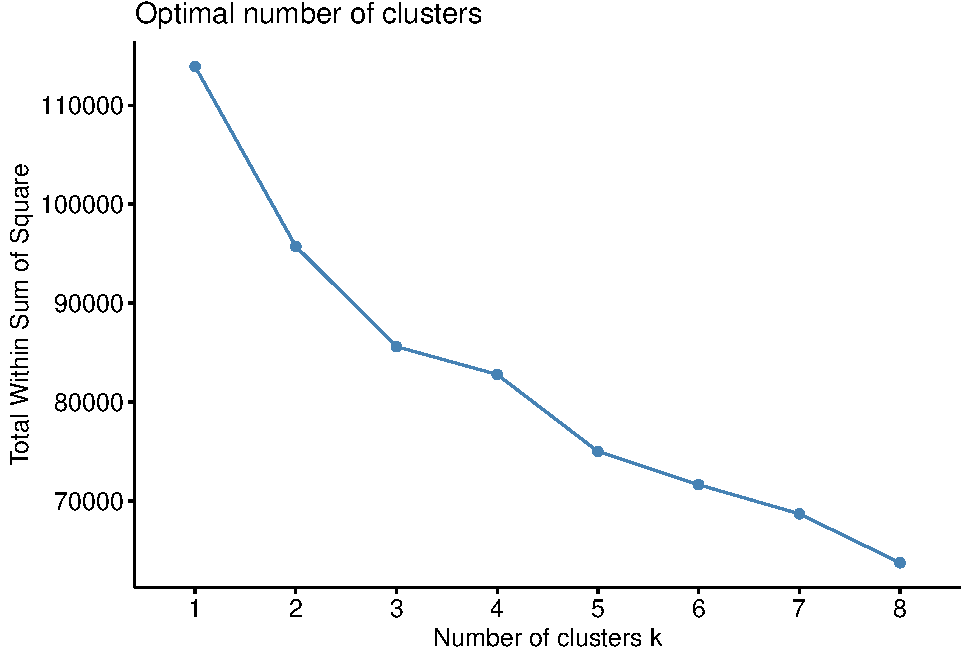
\includegraphics{imagenes/modelo_clusters/unnamed-chunk-15-2.pdf}
	%\includegraphics[width=0.25\textwidth]{mesh}
	\caption{Técnica Kmeans, Número óptimo de clusers, Criterio Suma de Cuadrados}
	\label{fig:kmeans_numoptimal_sumsquare}
\end{figure}

\clearpage



KMEANS y JERÁRQUICO analítico:\label{kmeas_jerarquico_numoptimal}

\begin{lstlisting}
## 
## Clustering Methods:
##  kmeans hierarchical 
## 
## Cluster sizes:
##  2 3 4 5 
## 
## Validation Measures:
##                                    2         3         4         5
##                                                                   
## kmeans       Connectivity     0.0000    3.1667  730.2742 1316.3881
##              Dunn             0.4693    0.5735    0.0471    0.0345
##              Silhouette       0.5937    0.5336    0.2070    0.1796
## hierarchical Connectivity     3.1667    3.1667    9.2357   12.1647
##              Dunn             0.5713    0.5735    0.2744    0.2744
##              Silhouette       0.7329    0.5336    0.5198    0.4879
## 
## Optimal Scores:
## 
##              Score  Method       Clusters
## Connectivity 0.0000 kmeans       2       
## Dunn         0.5735 kmeans       3       
## Silhouette   0.7329 hierarchical 2
\end{lstlisting}

\begin{itemize}
	\item
	Método Kmeans: Los resultados anteriores de validaciones internas,
	coinciden en que la óptima solución son 2 clusters en las
	métricas de Siloutte y Connectivity mientras que para la métrica de
	Dunn el óptimo número de clusters sería 3.
	\item
	Método Jerárquico: En esta validación se agregó el método jerárquico en el cual las métricas Connectivity y Dunn dan resultados iguales 	mientras que en silhouette es mejor el resultado con 2 clusters.
\end{itemize}

\paragraph{\textbf{tipo de cluster jerárquico:}}
Se realizan 4 cluster jerarquicos, cada uno utilizando las medidas de distancias ``complete'', ``average'', ``single'', ``ward''. Se calcula el coeficiente de correlación cophenético y se elige el de mayor valor. La tabla comparativa puede observarse a continuación \ref{tab:tabla_cophenetic_jerarquico}. En este caso la mejor opción es ``average''. 

\begin{table}[!h]
	
	\caption{\label{tab:tabla_cophenetic_jerarquico}Coef. cophenetic por cada tipo de cluster jerárquico}
	\centering
	\begin{tabular}[t]{lr}
		\toprule
		\rowcolor{black}  \multicolumn{1}{c}{\textcolor{white}{\textbf{metodo}}} & \multicolumn{1}{c}{\textcolor{white}{\textbf{coeficiente\_cofenetico}}}\\
		\midrule
		\rowcolor{gray!6}  complete & 0.7199776\\
		average & 0.8142721\\
		\rowcolor{gray!6}  single & 0.7217462\\
		ward & 0.3765082\\
		\bottomrule
	\end{tabular}
\end{table}



\paragraph{\textbf{Conclusión General}}
La conclusión es que la mejor opción es hacer clusters de 2 grupos ya sea por el método Kmeans o Jerárquico.


%-------------------------------------------------%
\subsubsection{\textbf{Modelar}}
%-------------------------------------------------%

\paragraph{\underline{\textbf{Cluster Kmeans}}}\label{cluster-kmeans}

Tomando como referencia las validaciones anteriores, se realiza un
cluster kmeans con 2 centroides. Este método se repetirá 25 veces
distintas y se elegirá el mejor.\\
Dicho procedimiento arroja resultados \ref{fig:kmeans_cluster_optimo} y \ref{fig:kmeans_cluster_optimo_silhouette}.

\begin{figure}[!htb]
	\centering
	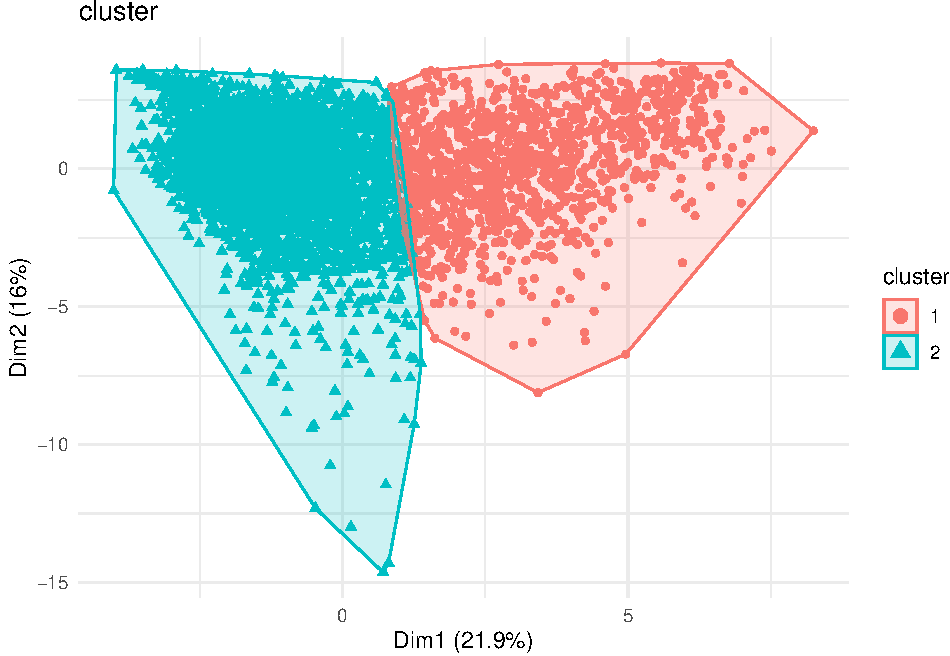
\includegraphics{imagenes/modelo_clusters/unnamed-chunk-18-1.pdf}
	%\includegraphics[width=0.25\textwidth]{mesh}
	\caption{Cluster óptimo Kmeans con 2 centroides. Variabilidad explicada 37.9\%}
	\label{fig:kmeans_cluster_optimo}
\end{figure}

\begin{figure}[!htb]
	\centering
	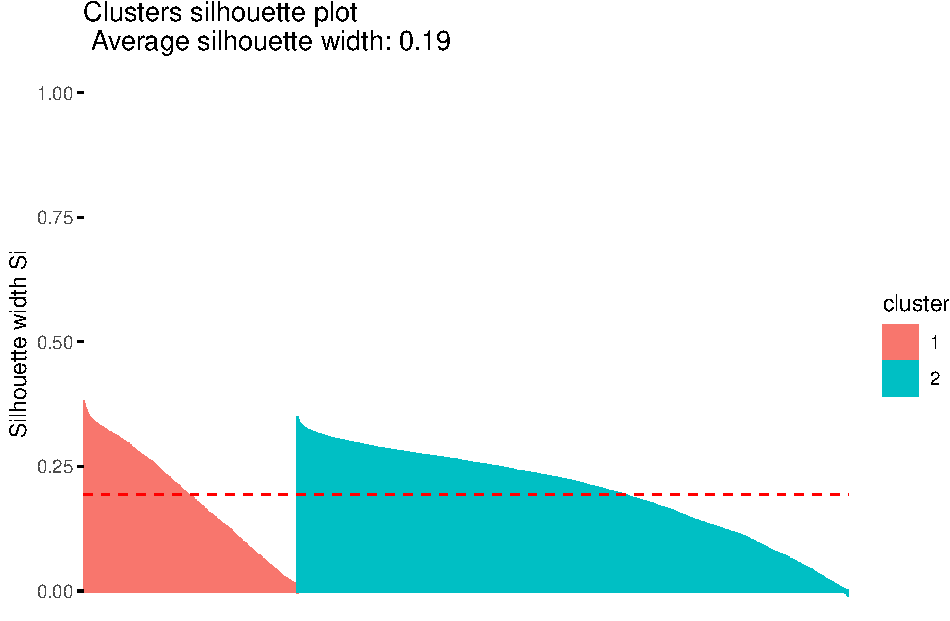
\includegraphics{imagenes/modelo_clusters/unnamed-chunk-18-2.pdf}
	%\includegraphics[width=0.25\textwidth]{mesh}
	\caption{Silhouette del cluster óptimo de kmeans \ref{fig:kmeans_cluster_optimo}}
	\label{fig:kmeans_cluster_optimo_silhouette}
\end{figure}


\clearpage


\hypertarget{cluster-jeruxe1rquico}{%
	\paragraph{\textbf{\underline{cluster jerárquico}}}\label{cluster-jeruxe1rquico}}
En este submodelo debido a la gran cantidad de observaciones, no podrá mostrarse el dendograma completo. Por lo tanto, el modelo se ejecuta y según lo sugerido en
las validaciones, se realiza el corte en 2 grupos. La composición puede observarse en la siguiente sección.


%-------------------------------------------------%
\subsubsection{\textbf{Describir el modelo}}
%-------------------------------------------------%

\paragraph{\textbf{Kmeans}}
El cluster kmeans modelado en la sección anterior parece ser muy bueno. Por lo tanto el próximo paso es saber en que cluster cae cada observación según su target para realizar una descripción de su composición según nuestra variable de interés.\\
La tabla \ref{tab:kmeans_2_resumen} y la figura \ref{fig:kmeans_cluster_optimo_composicion} resumen dicho análisis. Puede observarse que un grupo contiene solamente un 11,13\% de datos
erroneos, pero el otro grupo está muy balanceado. Por lo tanto, el
cluster de 2 grupos a pesar de que tenga muy buenos valores en las
validaciones realizadas, al verificar con el target real no da un buen resultado.

\begin{table}[!h]
	
	\caption{\label{tab:kmeans_2_resumen}Resumen composición de cluster Kmeans según clase desertor}
	\centering
	\resizebox{\linewidth}{!}{
	\begin{tabular}[t]{rrrrrr}
		\toprule
		\rowcolor{black}  \multicolumn{1}{c}{\textcolor{white}{\textbf{grupo}}} & \multicolumn{1}{c}{\textcolor{white}{\textbf{cant\_integrantes}}} & \multicolumn{1}{c}{\textcolor{white}{\textbf{cant\_desertores}}} & \multicolumn{1}{c}{\textcolor{white}{\textbf{cant\_desertores\_pct}}} & \multicolumn{1}{c}{\textcolor{white}{\textbf{cant\_no\_desertores}}} & \multicolumn{1}{c}{\textcolor{white}{\textbf{cant\_no\_desertores\_pct}}}\\
		\midrule
		\rowcolor{gray!6}  1 & 1275 & 142 & 11.13725 & 1133 & 88.86275\\
		2 & 3283 & 1858 & 56.59458 & 1425 & 43.40542\\
		\bottomrule
	\end{tabular}}
\end{table}


\begin{figure}[!htb]
	\centering
	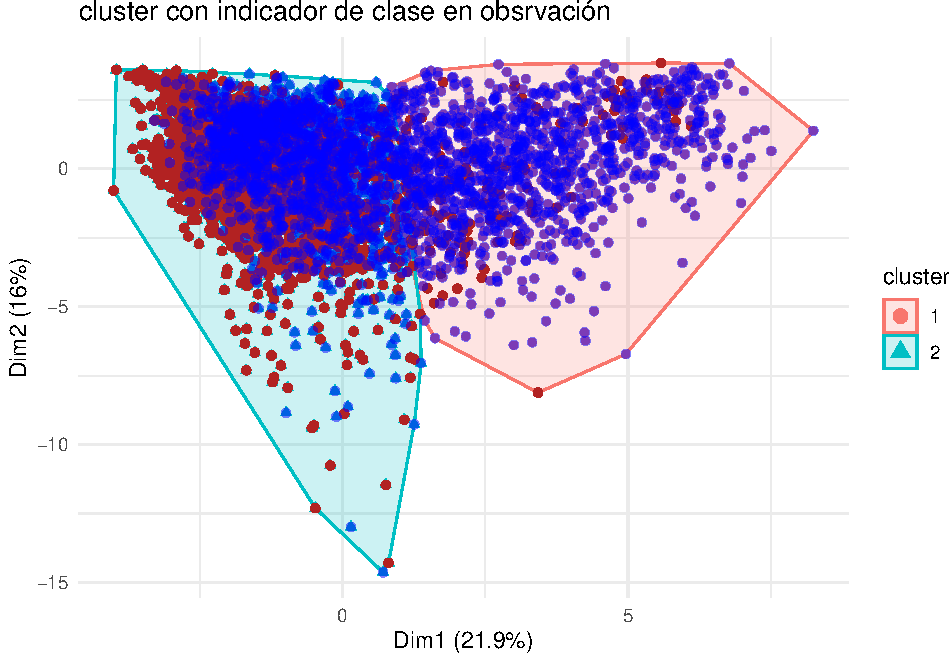
\includegraphics{imagenes/modelo_clusters/unnamed-chunk-21-1.pdf}
	%\includegraphics[width=0.25\textwidth]{mesh}
	\caption{Cluster óptimo Kmeans con 2 centroides. Variabilidad explicada 37.9\%. Indicación real de la clase}
	\label{fig:kmeans_cluster_optimo_composicion}
\end{figure}



\paragraph{\textbf{jerárquico}}

La composición de los grupos puede observarse en la tabla \ref{tab:tabla_jerarquico_composicion}. La misma detalla un grupo muy numeroso y otro muy chico y
ambos estan muy mezclados en función el target. Por lo tanto, el método
jerárquico no es adecuado.

\begin{table}[!h]
	
	\caption{\label{tab:tabla_jerarquico_composicion}Composición de clusters según la clase deserto}
	\centering
	\resizebox{\linewidth}{!}{
		\begin{tabular}[t]{rrrrrr}
			\toprule
			\rowcolor{black}  \multicolumn{1}{c}{\textcolor{white}{\textbf{grupo}}} & \multicolumn{1}{c}{\textcolor{white}{\textbf{cant\_integrantes}}} & \multicolumn{1}{c}{\textcolor{white}{\textbf{cant\_desertores}}} & \multicolumn{1}{c}{\textcolor{white}{\textbf{cant\_desertores\_pct}}} & \multicolumn{1}{c}{\textcolor{white}{\textbf{cant\_no\_desertores}}} & \multicolumn{1}{c}{\textcolor{white}{\textbf{cant\_no\_desertores\_pct}}}\\
			\midrule
			\rowcolor{gray!6}  1 & 4550 & 1996 & 43.86813 & 2554 & 56.13187\\
			2 & 8 & 4 & 50.00000 & 4 & 50.00000\\
			\bottomrule
	\end{tabular}}
\end{table}


\subsubsection{\textbf{Extensión de Clusters}}

A pesar del estudio de validaciones y resultados anteriormente,
se propone realizar varios modelos de cluster cambiando métodos y cantidad de grupos formados para estudiar los resultados. \\
De esta forma se pretende evaluar si existe algún modelo que sin importar la cantidad de grupos, represente mayoritariamente a las observaciones que lo componen según la clase deserto, la cual no es incluida para realizar los clusters.\\
La hipótesis es que como los resultados reales hacen referencia al target,
campo que no se incluye en los datos para hacer cluster al ser no
supervisado, podría darse el caso de que en la situación real otro
número de cluster sea óptima a la que arrojan las validaciones
matemáticas.\\

La tabla \ref{tab:tabla_muchos_clusters} y la figura \ref{fig:muchos_clusters} detallan los resultados de este experimento. La figura muestra la misma información que el cuadro anterior. En el eje
x indica que tipo de cluster es, cuantos clusters y la clase deserto
(``S'' y ``N''). En el eje y se indica el numero de cluster, por lo que
los cluster armados solo con 2 grupos, habrá información únicamente
hasta esa altura. Por ejemplo, para el caso de aplicar un método
jerárquico de 2 clusters podemos observar que en el primer cluster
tenemos 2554 casos Negatigos y 1996 casos positivos, mientras que el
cluster número 2 está conformado de 4 casos negativos y 4 casos
positivos.


\begin{table}[!h]
	
	\caption{\label{tab:tabla_muchos_clusters}Resumen por tipo de cluster, cantidad de clusters y la composición de cada uno según la clase deserto}
	\centering
	\resizebox{\linewidth}{!}{
		\begin{tabular}[t]{lrrrrrrrrrrr}
			\toprule
			\rowcolor{black}  \multicolumn{1}{c}{\textcolor{white}{\textbf{metodo}}} & \multicolumn{1}{c}{\textcolor{white}{\textbf{numero\_clusters}}} & \multicolumn{1}{c}{\textcolor{white}{\textbf{1\_N}}} & \multicolumn{1}{c}{\textcolor{white}{\textbf{1\_S}}} & \multicolumn{1}{c}{\textcolor{white}{\textbf{2\_N}}} & \multicolumn{1}{c}{\textcolor{white}{\textbf{2\_S}}} & \multicolumn{1}{c}{\textcolor{white}{\textbf{3\_N}}} & \multicolumn{1}{c}{\textcolor{white}{\textbf{3\_S}}} & \multicolumn{1}{c}{\textcolor{white}{\textbf{4\_N}}} & \multicolumn{1}{c}{\textcolor{white}{\textbf{4\_S}}} & \multicolumn{1}{c}{\textcolor{white}{\textbf{5\_N}}} & \multicolumn{1}{c}{\textcolor{white}{\textbf{5\_S}}}\\
			\midrule
			\rowcolor{gray!6}  jerarquico & 2 & 2554 & 1996 & 4 & 4 & NA & NA & NA & NA & NA & NA\\
			jerarquico & 3 & 2544 & 1972 & 10 & 24 & 4 & 4 & NA & NA & NA & NA\\
			\rowcolor{gray!6}  jerarquico & 4 & 2544 & 1970 & NA & 2 & 10 & 24 & 4 & 4 & NA & NA\\
			jerarquico & 5 & 2543 & 1970 & NA & 2 & 10 & 24 & 1 & NA & 4 & 4\\
			\rowcolor{gray!6}  kmeans & 2 & 1133 & 142 & 1425 & 1858 & NA & NA & NA & NA & NA & NA\\
			\addlinespace
			kmeans & 3 & 878 & 82 & 611 & 604 & 1069 & 1314 & NA & NA & NA & NA\\
			\rowcolor{gray!6}  kmeans & 4 & 1028 & 1252 & 842 & 73 & 14 & 28 & 674 & 647 & NA & NA\\
			kmeans & 5 & 725 & 576 & 400 & 837 & 606 & 487 & 14 & 28 & 813 & 72\\
			\bottomrule
	\end{tabular}}
\end{table}


\begin{figure}[!htb]
	\centering
	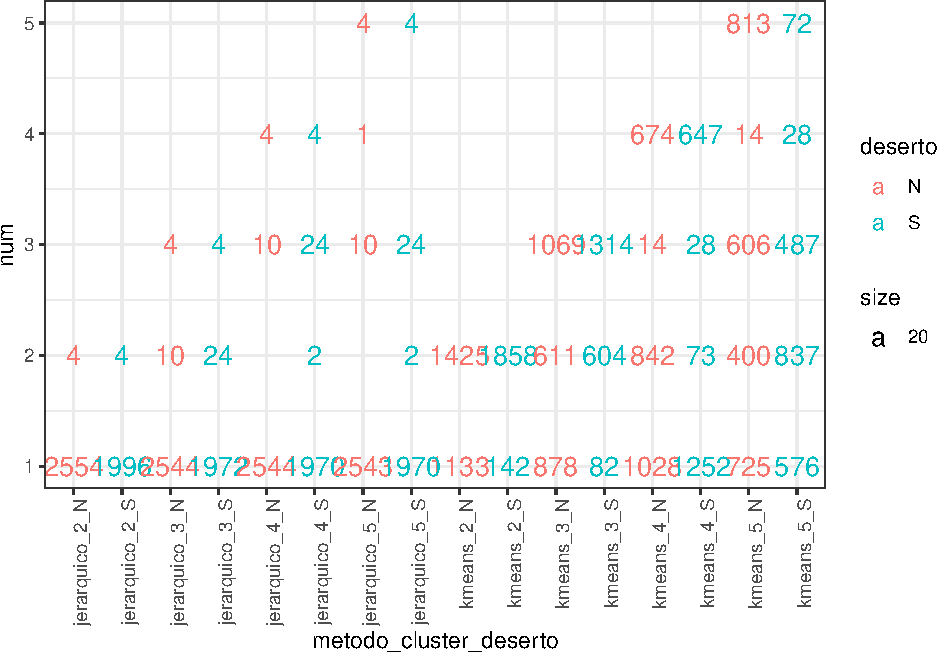
\includegraphics{imagenes/modelo_clusters/unnamed-chunk-25-1.pdf}
	%\includegraphics[width=0.25\textwidth]{mesh}
	\caption{Composición de muchos clusters distintos según target}
	\label{fig:muchos_clusters}
\end{figure}


\paragraph{\textbf{Conclusión general}}
la conclusión general es que ninguna de las variantes analizadas en este grid de clusters aún cambiando parámetro y métodos logra una identificación de grupos o subgrupos pertenecientes a alguna de las dos clases reales que hacen referencia a la deserción.\\






%-------------------------------------------------%
\subsection{Modelo: K-Nearest Neighbor (kNN)}
%-------------------------------------------------%
Vecinos mas cercanos:\\
Este algoritmo busca las ``k" observaciones mas parecidas del conjunto de entrenamiento al registro que se está evaluando que pertenece al conjunto de test. De esos k registros mas parecidos, se extrae la clase y cuyo valor sea el predominante, será el que se le otorgue al registro de Test.


%-------------------------------------------------%
\subsubsection{Determinar parámetros del modelo}
%-------------------------------------------------%
Éste método tiene un hiperparámentro solo (k), que hace referencia a la cantidad de registros vecinos que el algoritmo evaluará para luego clasificar según la clase predominante.\\

Para realizar el modelo se emplea validación cruzada con 10 particiones y 5 repeticiones. A su vez, cada iteración se repite con distintos valores del hiperparámetro k. En este caso se optaron por 6 valores: (1, 2, 5, 10, 15, 20, 30, 50, 60, 70, 80).\\
Entonces se puede decir que se realizan: 10*5*6 = 300 modelos, y de todos ellos se obtiene el mejor.

Las diferentes ejecuciones para elegir el parámetro óptimo se visualizan en la tabla \ref{tab:knn_corridas_parametros}.
Se puede determinar que el mejor resultado se obtiene con un k=70 y accuracy de 81,27\%.


\begin{table}[!h]
	
	\caption{\label{tab:knn_corridas_parametros} Ejecuciones de knn con diferentes parámetros}
	\centering
	\begin{tabular}[t]{rrrrr}
		\toprule
		\rowcolor{black}  \multicolumn{1}{c}{\textcolor{white}{\textbf{k}}} & \multicolumn{1}{c}{\textcolor{white}{\textbf{Accuracy}}} & \multicolumn{1}{c}{\textcolor{white}{\textbf{Kappa}}} & \multicolumn{1}{c}{\textcolor{white}{\textbf{AccuracySD}}} & \multicolumn{1}{c}{\textcolor{white}{\textbf{KappaSD}}}\\
		\midrule
		\rowcolor{gray!6}  1 & 0.7583 & 0.5077 & 0.0218 & 0.0451\\
		2 & 0.7535 & 0.4981 & 0.0216 & 0.0439\\
		\rowcolor{gray!6}  5 & 0.7956 & 0.5810 & 0.0202 & 0.0417\\
		10 & 0.7993 & 0.5877 & 0.0228 & 0.0477\\
		\rowcolor{gray!6}  15 & 0.8021 & 0.5937 & 0.0229 & 0.0476\\
		\addlinespace
		20 & 0.8033 & 0.5959 & 0.0204 & 0.0428\\
		\rowcolor{gray!6}  30 & 0.8049 & 0.5995 & 0.0209 & 0.0434\\
		50 & 0.8124 & 0.6144 & 0.0209 & 0.0437\\
		\rowcolor{gray!6}  60 & 0.8122 & 0.6140 & 0.0206 & 0.0430\\
		70 & 0.8127 & 0.6149 & 0.0209 & 0.0437\\
		\addlinespace
		\rowcolor{gray!6}  80 & 0.8096 & 0.6085 & 0.0224 & 0.0466\\
		\bottomrule
	\end{tabular}
\end{table}

\begin{figure}[!htb]
	\centering
	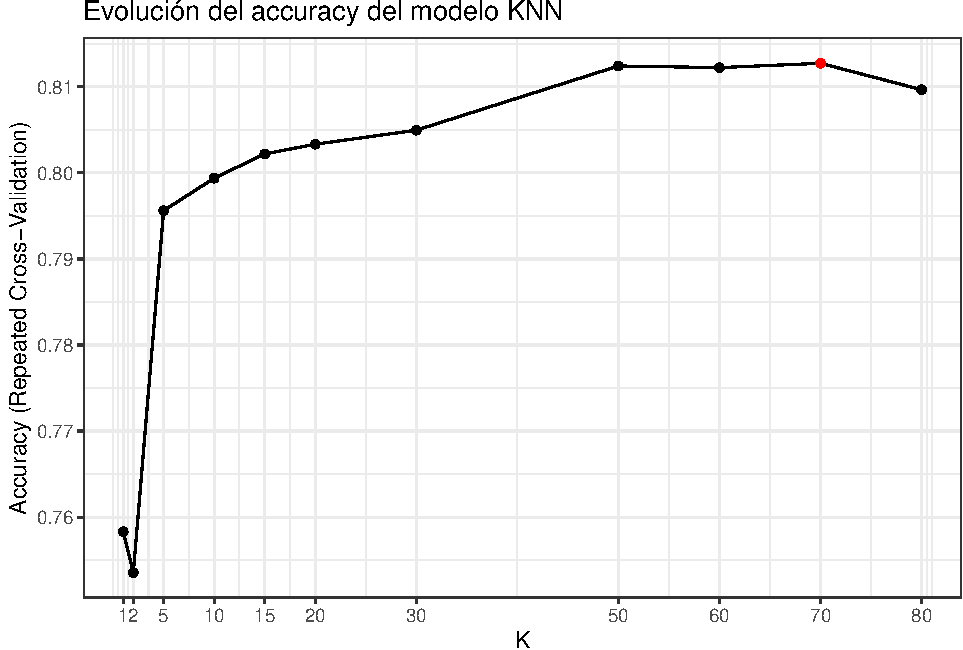
\includegraphics{imagenes/modelos_varios/unnamed-chunk-13-1.pdf}
	%\includegraphics[width=0.25\textwidth]{mesh}
	\caption{Evolución de Accuracy en modelos knn}
	\label{fig:knn_k_evolucion_accuracy}
\end{figure}


%-------------------------------------------------%
\subsubsection{Modelar}
%-------------------------------------------------%

Se ejecuta modelo de knn con k=70 utilizando todo el datset de train como entrenamiento (sin validación) obteniendo un accuracy de 81,98 \%, el cual es muy cercano al obtenido durante la búsqueda del parámetro óptimo (81,27\%)

%-------------------------------------------------%
\subsubsection{Describir el modelo}
%-------------------------------------------------%

Se evalúa el modelo anterior con el conjunto de Test cuyas observaciones no han sido utilizadas hasta ahora. Se detalla la Matriz de Confusión \ref{tab:MatrizConf_KNN} y algunas métricas \ref{tab:metricas_KNN}.

Como es de esperarse, los aciertos en el dataset de Test son menores que en el de entrenamiento. En este caso un 80.3 \% que sigue encontrándose muy por encima del nivel mínimo que corresponde a la
clase mayoritaria (56\%)



\begin{table}[!h]
	
	\caption{\label{tab:MatrizConf_KNN}Matriz de Confusión del método: KNN }
	\centering
	\begin{tabular}[t]{lcc}
		\toprule
		\multicolumn{1}{c}{Prediccion} & \multicolumn{1}{c}{Referencia} & \multicolumn{1}{c}{ } \\
		\cmidrule(l{3pt}r{3pt}){1-1} \cmidrule(l{3pt}r{3pt}){2-2}
		\rowcolor{black}  \multicolumn{1}{c}{\textcolor{white}{\textbf{ }}} & \multicolumn{1}{c}{\textcolor{white}{\textbf{0}}} & \multicolumn{1}{c}{\textcolor{white}{\textbf{1}}}\\
		\midrule
		\rowcolor{gray!6}  0 & 657 & 160\\
		1 & 110 & 440\\
		\bottomrule
	\end{tabular}
\end{table}

\begin{table}[!h]
	
	\caption{\label{tab:metricas_KNN}Métricas del metodo: KNN }
	\centering
	\begin{tabular}[t]{cc}
		\toprule
		\rowcolor{black}  \multicolumn{1}{c}{\textcolor{white}{\textbf{metricas}}} & \multicolumn{1}{c}{\textcolor{white}{\textbf{valor}}}\\
		\midrule
		\rowcolor{gray!6}  Accuracy & 0.8024\\
		Kappa & 0.5953\\
		\rowcolor{gray!6}  AccuracyLower & 0.7803\\
		AccuracyUpper & 0.8232\\
		\rowcolor{gray!6}  AccuracyNull & 0.5610\\
		\addlinespace
		AccuracyPValue & 0.0000\\
		\rowcolor{gray!6}  McnemarPValue & 0.0028\\
		Sensitivity & 0.7333\\
		\rowcolor{gray!6}  Specificity & 0.8565\\
		Pos Pred Value & 0.8000\\
		\addlinespace
		\rowcolor{gray!6}  Neg Pred Value & 0.8041\\
		Precision & 0.8000\\
		\rowcolor{gray!6}  Recall & 0.7333\\
		F1 & 0.7652\\
		\rowcolor{gray!6}  Prevalence & 0.4389\\
		\addlinespace
		Detection Rate & 0.3218\\
		\rowcolor{gray!6}  Detection Prevalence & 0.4023\\
		Balanced Accuracy & 0.7949\\
		\bottomrule
	\end{tabular}
\end{table}



%-------------------------------------------------%
\subsection{Modelo: Regresión Logística}
%-------------------------------------------------%

La Regresión logística permite estimar la probabilidad de una variable cualitativa binaria en
función de variables cuantitativas. Es un algoritmo que puede explicar
bien la respuesta en función de sus predictores. La relación como lo
dice su nombre es logarítmica, por lo que la relación entre las
probabilidades y las variables no es lineal. El incremento en 1 unidad de
una variable depende también del valor que tiene la variable en ese
momento (es decir, la posición en la curva logarítmica donde se
encuentra).

%-------------------------------------------------%
\subsubsection{Determinar parámetros del modelo}
%-------------------------------------------------%
No existen hiperparámetros. Como en este caso se utiliza el paquete glm,
hay que determinar que se realiza una regresión logística indicando
que el paquete utilice la familia binomial.


%-------------------------------------------------%
\subsubsection{Modelar}
%-------------------------------------------------%

Se ejecuta el modelo obteniendo durante el entrenamiento un Accuracy de 83.7\%.\\

No todas las variables son significativas, lo que
nos lleva a pensar que algunas variables están aportando la misma información.



%-------------------------------------------------%
\subsubsection{Describir el modelo}
%-------------------------------------------------%


Se evalúa el modelo entrenado con el conjunto de Test. En este caso, se
puede observar \ref{tab:MatrizConf_logistic} \ref{tab:metricas_logistic} que el modelo resulta ser bastante robusto obteniendo
casi el mismo valor en Accuracy que el modelo entrenado, 83,54\%. Es un
buen modelo para tener en cuenta y analizarlo mas en profundidad.

\begin{table}[!h]
	
	\caption{\label{tab:MatrizConf_logistic}Matriz de Confusión del metodo: Regresión Logística (todos los predictores) }
	\centering
	\begin{tabular}[t]{lcc}
		\toprule
		\multicolumn{1}{c}{Predicción} & \multicolumn{1}{c}{Referencia} & \multicolumn{1}{c}{ } \\
		\cmidrule(l{3pt}r{3pt}){1-1} \cmidrule(l{3pt}r{3pt}){2-2}
		\rowcolor{black}  \multicolumn{1}{c}{\textcolor{white}{\textbf{ }}} & \multicolumn{1}{c}{\textcolor{white}{\textbf{0}}} & \multicolumn{1}{c}{\textcolor{white}{\textbf{1}}}\\
		\midrule
		\rowcolor{gray!6}  0 & 702 & 160\\
		1 & 65 & 440\\
		\bottomrule
	\end{tabular}
\end{table}

\begin{table}[!h]
	
	\caption{\label{tab:metricas_logistic}Métricas del método: logistic }
	\centering
	\begin{tabular}[t]{cc}
		\toprule
		\rowcolor{black}  \multicolumn{1}{c}{\textcolor{white}{\textbf{metricas}}} & \multicolumn{1}{c}{\textcolor{white}{\textbf{valor}}}\\
		\midrule
		\rowcolor{gray!6}  Accuracy & 0.8354\\
		Kappa & 0.6599\\
		\rowcolor{gray!6}  AccuracyLower & 0.8146\\
		AccuracyUpper & 0.8546\\
		\rowcolor{gray!6}  AccuracyNull & 0.5610\\
		\addlinespace
		AccuracyPValue & 0.0000\\
		\rowcolor{gray!6}  McnemarPValue & 0.0000\\
		Sensitivity & 0.7333\\
		\rowcolor{gray!6}  Specificity & 0.9152\\
		Pos Pred Value & 0.8712\\
		\addlinespace
		\rowcolor{gray!6}  Neg Pred Value & 0.8143\\
		Precision & 0.8712\\
		\rowcolor{gray!6}  Recall & 0.7333\\
		F1 & 0.7963\\
		\rowcolor{gray!6}  Prevalence & 0.4389\\
		\addlinespace
		Detection Rate & 0.3218\\
		\rowcolor{gray!6}  Detection Prevalence & 0.3694\\
		Balanced Accuracy & 0.8242\\
		\bottomrule
	\end{tabular}
\end{table}




%-------------------------------------------------%
\subsection{Modelo: Analisis discriminante Lineal
	(LDA)}
%-------------------------------------------------%

Este algoritmo utiliza el teorema de Bayes, para estimar la probabilidad
de que una observación pertenezca a cada una de las clases de la
variable cualitativa según el valor de los predictores. Es un algoritmo
explicativo y puede discriminar mas de dos clases, aunque este no sea el
caso. En primer lugar, se calculan las probabilidades de
pertenencia de la observación a cada una de las clases y luego se asigna la clase cuya probabilidad resulta la mas alta.



%-------------------------------------------------%
\subsubsection{Determinar parámetros del modelo}
%-------------------------------------------------%

No tiene.


%-------------------------------------------------%
\subsubsection{Modelar}
%-------------------------------------------------%

Utilizando el conjunto de entrenamiento, se obtiene una métrica Accuracy del 82.6\%


%-------------------------------------------------%
\subsubsection{Describir el modelo}
%-------------------------------------------------%

Evaluando el modelo con el conjunto de Test, el modelo aparenta ser
bastante robusto obteniendo casi el mismo valor en Accuracy (82.26\%)
que en entrenamiento (82.6\%). \ref{tab:MatrizConf_LDA} \ref{tab:metricas_LDA}

\begin{table}[!h]
	
	\caption{\label{tab:MatrizConf_LDA}Matriz de Confusion del metodo: LDA }
	\centering
	\begin{tabular}[t]{lcc}
		\toprule
		\multicolumn{1}{c}{Prediccion} & \multicolumn{1}{c}{Referencia} & \multicolumn{1}{c}{ } \\
		\cmidrule(l{3pt}r{3pt}){1-1} \cmidrule(l{3pt}r{3pt}){2-2}
		\rowcolor{black}  \multicolumn{1}{c}{\textcolor{white}{\textbf{ }}} & \multicolumn{1}{c}{\textcolor{white}{\textbf{0}}} & \multicolumn{1}{c}{\textcolor{white}{\textbf{1}}}\\
		\midrule
		\rowcolor{gray!6}  0 & 704 & 174\\
		1 & 63 & 426\\
		\bottomrule
	\end{tabular}
\end{table}

\begin{table}[!h]
	
	\caption{\label{tab:metricas_LDA}Métricas del metodo: LDA }
	\centering
	\begin{tabular}[t]{cc}
		\toprule
		\rowcolor{black}  \multicolumn{1}{c}{\textcolor{white}{\textbf{metricas}}} & \multicolumn{1}{c}{\textcolor{white}{\textbf{valor}}}\\
		\midrule
		\rowcolor{gray!6}  Accuracy & 0.8266\\
		Kappa & 0.6407\\
		\rowcolor{gray!6}  AccuracyLower & 0.8054\\
		AccuracyUpper & 0.8463\\
		\rowcolor{gray!6}  AccuracyNull & 0.5610\\
		\addlinespace
		AccuracyPValue & 0.0000\\
		\rowcolor{gray!6}  McnemarPValue & 0.0000\\
		Sensitivity & 0.7100\\
		\rowcolor{gray!6}  Specificity & 0.9178\\
		Pos Pred Value & 0.8711\\
		\addlinespace
		\rowcolor{gray!6}  Neg Pred Value & 0.8018\\
		Precision & 0.8711\\
		\rowcolor{gray!6}  Recall & 0.7100\\
		F1 & 0.7823\\
		\rowcolor{gray!6}  Prevalence & 0.4389\\
		\addlinespace
		Detection Rate & 0.3116\\
		\rowcolor{gray!6}  Detection Prevalence & 0.3577\\
		Balanced Accuracy & 0.8139\\
		\bottomrule
	\end{tabular}
\end{table}



%-------------------------------------------------%
\subsection{Modelo: Árbol de Clasificación simple}
%-------------------------------------------------%

Se emplea el algoritmo de arboles de decisión C5.0. Los árboles son
fáciles de interpretar aun cuando las relaciones entre predictores son
complejas. Se pueden leer las ramas del árbol e interpretarlas como reglas para clasificar a cualquier observación.

%-------------------------------------------------%
\subsubsection{Determinar parámetros del modelo}
%-------------------------------------------------%

Si bien en estos algoritmos existen parámetros como cantidad de
observaciones en los nodos finales, máximo nivel de profundidad, etc. En este caso no se empleará ninguno dejando que el algoritmo determine cual es mejor corte en los mismos.

%-------------------------------------------------%
\subsubsection{Modelar}
%-------------------------------------------------%

Finalizado el entrenamiento, el Accuracy informado es del 85,52\%.

\begin{lstlisting}
## Decision tree:
## 
## ciclo_lectivo_de_cursada <= -0.1784513:
## :...Aprobado <= 2.816905: 1 (889/45)
## :   Aprobado > 2.816905: 0 (26/2)
## ciclo_lectivo_de_cursada > -0.1784513:
## :...Aprobado > 0.1499444: 0 (819/56)
##     Aprobado <= 0.1499444:
##     :...tipo_de_aprobacion_libre <= -0.1299698:
##         :...tipo_de_aprobacion_firmo <= -1.007704: 1 (64/26)
##         :   tipo_de_aprobacion_firmo > -1.007704: 0 (834/150)
##         tipo_de_aprobacion_libre > -0.1299698:
##         :...noAprobado > 0.6500659: 0 (56/17)
##             noAprobado <= 0.6500659:
##             :...Aprobado <= -0.5414899: 1 (281/94)
##                 Aprobado > -0.5414899:
##                 :...cant_recursada_regular_Recurso4vez > -0.2406067: 1 (40/12)
##                     cant_recursada_regular_Recurso4vez <= -0.2406067:
##                     :...tipo_de_aprobacion_libre > 1.48903: 1 (36/12)
##                         tipo_de_aprobacion_libre <= 1.48903:
##                         :...EsTecnico_SinDato <= 0: 0 (124/40)
##                             EsTecnico_SinDato > 0: 1 (22/8)
\end{lstlisting}

%-------------------------------------------------%
\subsubsection{Describir el modelo}
%-------------------------------------------------%

Evaluando el árbol con el conjunto de test, se obtiene un 83,24 \% de Accuracy. \ref{tab:MatrizConf_arbol} \ref{tab:metricas_arbol}

\begin{table}[!h]
	
	\caption{\label{tab:MatrizConf_arbol}Matriz de Confusión del método: árbol }
	\centering
	\begin{tabular}[t]{lcc}
		\toprule
		\multicolumn{1}{c}{Prediccion} & \multicolumn{1}{c}{Referencia} & \multicolumn{1}{c}{ } \\
		\cmidrule(l{3pt}r{3pt}){1-1} \cmidrule(l{3pt}r{3pt}){2-2}
		\rowcolor{black}  \multicolumn{1}{c}{\textcolor{white}{\textbf{ }}} & \multicolumn{1}{c}{\textcolor{white}{\textbf{0}}} & \multicolumn{1}{c}{\textcolor{white}{\textbf{1}}}\\
		\midrule
		\rowcolor{gray!6}  0 & 666 & 128\\
		1 & 101 & 472\\
		\bottomrule
	\end{tabular}
\end{table}

\begin{table}[!h]
	
	\caption{\label{tab:metricas_arbol}Métricas del método: arbol }
	\centering
	\begin{tabular}[t]{cc}
		\toprule
		\rowcolor{black}  \multicolumn{1}{c}{\textcolor{white}{\textbf{metricas}}} & \multicolumn{1}{c}{\textcolor{white}{\textbf{valor}}}\\
		\midrule
		\rowcolor{gray!6}  Accuracy & 0.8324\\
		Kappa & 0.6582\\
		\rowcolor{gray!6}  AccuracyLower & 0.8116\\
		AccuracyUpper & 0.8519\\
		\rowcolor{gray!6}  AccuracyNull & 0.5610\\
		\addlinespace
		AccuracyPValue & 0.0000\\
		\rowcolor{gray!6}  McnemarPValue & 0.0857\\
		Sensitivity & 0.7866\\
		\rowcolor{gray!6}  Specificity & 0.8683\\
		Pos Pred Value & 0.8237\\
		\addlinespace
		\rowcolor{gray!6}  Neg Pred Value & 0.8387\\
		Precision & 0.8237\\
		\rowcolor{gray!6}  Recall & 0.7866\\
		F1 & 0.8047\\
		\rowcolor{gray!6}  Prevalence & 0.4389\\
		\addlinespace
		Detection Rate & 0.3452\\
		\rowcolor{gray!6}  Detection Prevalence & 0.4191\\
		Balanced Accuracy & 0.8274\\
		\bottomrule
	\end{tabular}
\end{table}


%-------------------------------------------------%
\subsection{Modelo: Random Forest}
%-------------------------------------------------%

Este algoritmo combina el proceso de bagging (bootstrap aggregation
-muestras de observaciones con repetición-) con distintos modelos de
árboles que toman features al azar. Al final promedia los modelos y
consigue reducir la varianza.


%-------------------------------------------------%
\subsubsection{Determinar parámetros del modelo}
%-------------------------------------------------%

Se utiliza el paquete ranger en el cual se pueden definir los siguientes
hiperparámetros:

\begin{itemize}
	\item
	mtry: número predictores seleccionados aleatoriamente en cada árbol.
	Se eligen para evaluar los valores: 3, 4, 5, 7.
	\item
	min.node.size: tamaño mínimo que tiene que tener un nodo para poder
	ser dividido. Se eligen para evaluar los valores: 2, 3, 4, 5, 10, 15,
	20, 30.
	\item
	splitrule: criterio de división. El criterio elegido es ``gini''.
\end{itemize}

El mejor modelo determinado queda con los siguientes parámetros: mtry=5,
splitrule=gini y
 min.node.size=30 según la evolución del accuracy \ref{fig:rf_hiperparam}


\begin{figure}[!htb]
	\centering
	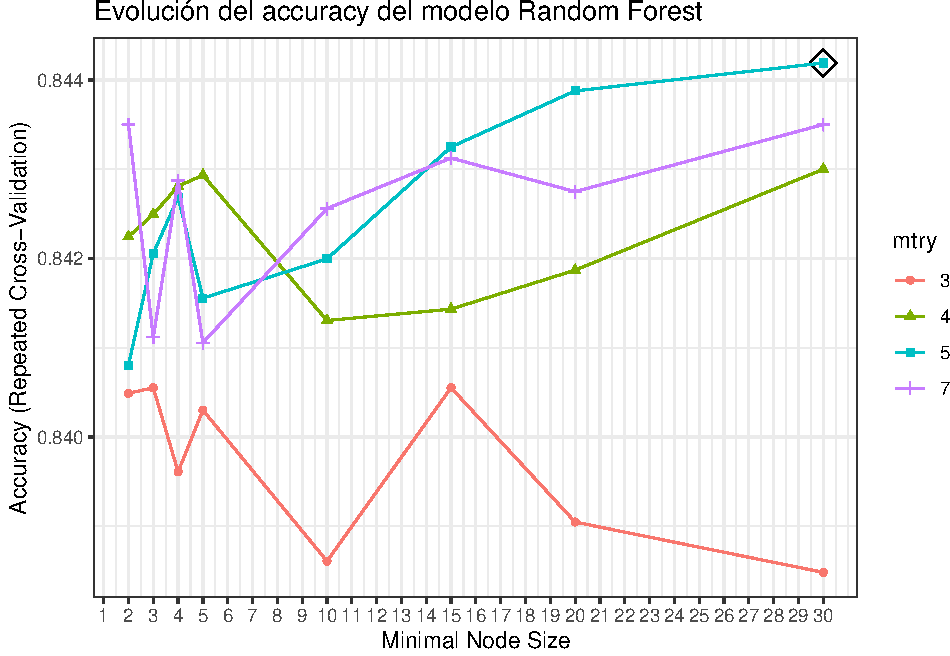
\includegraphics{imagenes/modelos_varios/unnamed-chunk-24-1.pdf}
	%\includegraphics[width=0.25\textwidth]{mesh}
	\caption{Evolución de Accuracy en modelos Random Forest para determinar hiperparámetros}
	\label{fig:rf_hiperparam}
\end{figure}



%-------------------------------------------------%
\subsubsection{Modelar}
%-------------------------------------------------%
El mejor modelo determinado con los hiperparmétros queda guardado y se ejecuta nuevamente utilizando todo el conjunto como train obteniendo un Accuracy del 92\%. Hay que tener en cuenta que este mismo modelo y con el mismo conjunto de datos (train) pero realizando cross-validation, logra un Accuracy de 84.3\%, por lo que puede señalar un sobreajuste. Sin embargo lo determinará la comparación con el conjunto de Test. \\

%\begin{table}[!h]
%	
%	\caption{\label{tab:MatrizConf_RandomForest-Train}Matriz de Confusion del metodo: RandomForest-Train }
%	\centering
%	\begin{tabular}[t]{lcc}
%		\toprule
%		\multicolumn{1}{c}{Prediccion} & \multicolumn{1}{c}{Referencia} & \multicolumn{1}{c}{ } \\
%		\cmidrule(l{3pt}r{3pt}){1-1} \cmidrule(l{3pt}r{3pt}){2-2}
%		\rowcolor{black}  \multicolumn{1}{c}{\textcolor{white}{\textbf{ }}} & \multicolumn{1}{c}{\textcolor{white}{\textbf{0}}} & \multicolumn{1}{c}{\textcolor{white}{\textbf{1}}}\\
%		\midrule
%		\rowcolor{gray!6}  0 & 1589 & 202\\
%		1 & 299 & 1101\\
%		\bottomrule
%	\end{tabular}
%\end{table}





%-------------------------------------------------%
\subsubsection{Describir el modelo}
%-------------------------------------------------%

Se realiza la evaluación del modelo con el conjunto de Test. En esta
corrida se obtiene un accuracy de 83.83\% \ref{tab:MatrizConf_rf} \ref{tab:metricas_rf} . Un valor muy cercano a los valores obtenidos con train-validation pero un poco alejado del mismo modelo pero sin usar subconjunto validación. Por lo que indica un poco de sobreajuste en el entrenamiento del modelo final.\\


\begin{table}[!h]
	
	\caption{\label{tab:MatrizConf_rf}Matriz de Confusion del metodo: rf }
	\centering
	\begin{tabular}[t]{lcc}
		\toprule
		\multicolumn{1}{c}{Prediccion} & \multicolumn{1}{c}{Referencia} & \multicolumn{1}{c}{ } \\
		\cmidrule(l{3pt}r{3pt}){1-1} \cmidrule(l{3pt}r{3pt}){2-2}
		\rowcolor{black}  \multicolumn{1}{c}{\textcolor{white}{\textbf{ }}} & \multicolumn{1}{c}{\textcolor{white}{\textbf{0}}} & \multicolumn{1}{c}{\textcolor{white}{\textbf{1}}}\\
		\midrule
		\rowcolor{gray!6}  0 & 681 & 135\\
		1 & 86 & 465\\
		\bottomrule
	\end{tabular}
\end{table}

\begin{table}[!h]
	
	\caption{\label{tab:metricas_rf}Métricas del método: rf }
	\centering
	\begin{tabular}[t]{cc}
		\toprule
		\rowcolor{black}  \multicolumn{1}{c}{\textcolor{white}{\textbf{metricas}}} & \multicolumn{1}{c}{\textcolor{white}{\textbf{valor}}}\\
		\midrule
		\rowcolor{gray!6}  Accuracy & 0.8383\\
		Kappa & 0.6688\\
		\rowcolor{gray!6}  AccuracyLower & 0.8177\\
		AccuracyUpper & 0.8574\\
		\rowcolor{gray!6}  AccuracyNull & 0.5610\\
		\addlinespace
		AccuracyPValue & 0.0000\\
		\rowcolor{gray!6}  McnemarPValue & 0.0012\\
		Sensitivity & 0.7750\\
		\rowcolor{gray!6}  Specificity & 0.8878\\
		Pos Pred Value & 0.8439\\
		\addlinespace
		\rowcolor{gray!6}  Neg Pred Value & 0.8345\\
		Precision & 0.8439\\
		\rowcolor{gray!6}  Recall & 0.7750\\
		F1 & 0.8079\\
		\rowcolor{gray!6}  Prevalence & 0.4389\\
		\addlinespace
		Detection Rate & 0.3401\\
		\rowcolor{gray!6}  Detection Prevalence & 0.4030\\
		Balanced Accuracy & 0.8314\\
		\bottomrule
	\end{tabular}
\end{table}


%-------------------------------------------------%
\subsection{Modelo: Gradient Boosting}
%-------------------------------------------------%

Boosting es una de las estrategias que hay de ensemble que se pueden
aplicar a muchos métodos, entre ellos los árboles. Boosting ajusta de
forma secuencial múltiples modelos en cadena. Cada nuevo modelo emplea
información del modelo anterior para aprender de sus errores, mejorando
iteración a iteración. Este método utiliza todos los features en todos los modelos.


%-------------------------------------------------%
\subsubsection{Determinar parámetros del modelo}
%-------------------------------------------------%

Estos métodos se caracterizan por tener muchos hiperparámetros y
parámetros. En este caso se utiliza el paquete gbm y dentro de el se
pueden emplear los siguientes:

\begin{itemize}
	\item
	n.trees: número de iteraciones del algoritmo de boosting (cantidad de
	modelos que forman el ensemble). Cuanto mas grande, mas riesgo de
	sobreajuste. Se prueban los siguientes valores: 100, 500, 1000, 2000.
	\item
	interaction.depth: complejidad de los árboles (cantidad total de
	divisiones que tiene el árbol). Se prueban los siguientes valores: 1,
	5, 9.
	\item
	shrinkage: (learning rate) controla la influencia que tiene cada modelo
	sobre el conjunto del ensemble (aprendizaje). Los valores que se
	probaron son: 0.001, 0.01, 0.1.
	\item
	n.minobsinnode: número mínimo de observaciones que debe tener un nodo
	para poder ser dividido. Se probaron los siguientes valores: 2, 10, 20.
	\item
	distribution: determina la función de coste (loss function). Se utiliza
	Adaboost.
	\item
	bag.fraction (subsampling fraction): Si es de 1, se emplea Gradient
	Boosting, si es menor que 1, se emplea Stochastic Gradient Boosting. Por
	defecto su valor es de 0.5. Se utiliza valor por defecto.
\end{itemize}

La combinación de hiperparámetros
que por una escasa diferencia sobrepasa al resto, es: n.trees = 500,
interaction.depth = 9, shrinkage = 0.01 y n.minobsinnode = 10


\begin{figure}[!htb]
	\centering
	\includegraphics[width=0.9\textwidth]{imagenes/modelos_varios/unnamed-chunk-28-1.pdf}
	%\includegraphics[width=0.25\textwidth]{mesh}
	\caption{Evolución de Accuracy en modelos Gradient Boosting para determinar hiperparámetros}
	\label{fig:rf_hiperparam}
\end{figure}


%-------------------------------------------------%
\subsubsection{Modelar}
%-------------------------------------------------%

En este caso pasa algo similar que con RandomForest. Cuando se usa el conjunto de entrenamiento para generar modelos mediante cross-validation con los hiperparámetros optimizados, se obtiene un Accuracy promedio del 84,34\%. Sin embargo, cuando este mismo métodos y utilizando los mismos hiperparámetros se emplea sin subdivisión de validación (usando todo el conjunto como train), se obtiene un accuracy del 87,4\%. Por lo tanto, está un poco sobreajustado pero no hay tanta diferencia como lo era con RandomForest.





%-------------------------------------------------%
\subsubsection{Describir el modelo}
%-------------------------------------------------%

Se evalúa el modelo con el conjunto de Test. En esta oportunidad se obtiene  Accuracy de 83.83\%. \ref{tab:MatrizConf_boosting} \ref{tab:metricas_boosting}

\begin{table}[!h]
	
	\caption{\label{tab:MatrizConf_boosting}Matriz de Confusión del método: boosting }
	\centering
	\begin{tabular}[t]{lcc}
		\toprule
		\multicolumn{1}{c}{Prediccion} & \multicolumn{1}{c}{Referencia} & \multicolumn{1}{c}{ } \\
		\cmidrule(l{3pt}r{3pt}){1-1} \cmidrule(l{3pt}r{3pt}){2-2}
		\rowcolor{black}  \multicolumn{1}{c}{\textcolor{white}{\textbf{ }}} & \multicolumn{1}{c}{\textcolor{white}{\textbf{0}}} & \multicolumn{1}{c}{\textcolor{white}{\textbf{1}}}\\
		\midrule
		\rowcolor{gray!6}  0 & 678 & 135\\
		1 & 89 & 465\\
		\bottomrule
	\end{tabular}
\end{table}

\begin{table}[!h]
	
	\caption{\label{tab:metricas_boosting}Métricas del método: boosting }
	\centering
	\begin{tabular}[t]{cc}
		\toprule
		\rowcolor{black}  \multicolumn{1}{c}{\textcolor{white}{\textbf{metricas}}} & \multicolumn{1}{c}{\textcolor{white}{\textbf{valor}}}\\
		\midrule
		\rowcolor{gray!6}  Accuracy & 0.8361\\
		Kappa & 0.6645\\
		\rowcolor{gray!6}  AccuracyLower & 0.8154\\
		AccuracyUpper & 0.8553\\
		\rowcolor{gray!6}  AccuracyNull & 0.5610\\
		\addlinespace
		AccuracyPValue & 0.0000\\
		\rowcolor{gray!6}  McnemarPValue & 0.0026\\
		Sensitivity & 0.7750\\
		\rowcolor{gray!6}  Specificity & 0.8839\\
		Pos Pred Value & 0.8393\\
		\addlinespace
		\rowcolor{gray!6}  Neg Pred Value & 0.8339\\
		Precision & 0.8393\\
		\rowcolor{gray!6}  Recall & 0.7750\\
		F1 & 0.8058\\
		\rowcolor{gray!6}  Prevalence & 0.4389\\
		\addlinespace
		Detection Rate & 0.3401\\
		\rowcolor{gray!6}  Detection Prevalence & 0.4052\\
		Balanced Accuracy & 0.8294\\
		\bottomrule
	\end{tabular}
\end{table}



%-------------------------------------------------%
\subsection{Modelo: Support Vector machine (SVM)}
%-------------------------------------------------%

Este algoritmo se basa en la separación de las clases con hiperplanos y
utilizando kernels para aumentar las dimensiones.

%-------------------------------------------------%
\subsubsection{Determinar parámetros del modelo}
%-------------------------------------------------%
Se utiliza el paquete kernlab que tiene 2 hiperparámetros:

\begin{itemize}
	\item
	sigma: coeficiente del kernel radial. Se prueban los valores: 0.001,
	0.01, 0.1, 0.5, 1.
	\item
	C: penalización por violaciones del margen del hiperplano. se prueban
	los valores: 1, 20, 50, 100, 200, 500, 700.
\end{itemize}

Los mejores resultados a través de las iteraciones de los modelos
generados fue con los valores: sigma = 0.001 y C = 100. Los mismos se
contrastan con los valores de Accuracy obtenidos en cada modelo y cuya
evolución puede verse en el grafico \ref{fig:svm_hiperparam}.



\begin{figure}[!htb]
	\centering
	\includegraphics[width=0.78\textwidth]{imagenes/modelos_varios/unnamed-chunk-32-1.pdf}
	%\includegraphics[width=0.25\textwidth]{mesh}
	\caption{Evolución de Accuracy en modelos SVM para determinar hiperparámetros}
	\label{fig:svm_hiperparam}
\end{figure}



%-------------------------------------------------%
\subsubsection{Modelar}
%-------------------------------------------------%

En entrenamiento se consigue un Accuracy de 83.79\% (con validation) y
85.11\% sin validación. Aparenta ser un modelo robusto.


%-------------------------------------------------%
\subsubsection{Describir el modelo}
%-------------------------------------------------%

Evaluando en el conjunto de Test se obtiene 84.2\% de Accuracy. Es el Modelo que mejor resultados da con esta métrica y además es robusto. Para mas información del modelo se detalla la Matriz de Confusión \ref{tab:MatrizConf_SVMradial} y Algunas métricas \ref{tab:metricas_SVMradial}.

\begin{table}[!h]
	
	\caption{\label{tab:metricas_SVMradial}Métricas del metodo: SVMradial }
	\centering
	\begin{tabular}[t]{cc}
		\toprule
		\rowcolor{black}  \multicolumn{1}{c}{\textcolor{white}{\textbf{metricas}}} & \multicolumn{1}{c}{\textcolor{white}{\textbf{valor}}}\\
		\midrule
		\rowcolor{gray!6}  Accuracy & 0.8419\\
		Kappa & 0.6732\\
		\rowcolor{gray!6}  AccuracyLower & 0.8215\\
		AccuracyUpper & 0.8609\\
		\rowcolor{gray!6}  AccuracyNull & 0.5610\\
		\addlinespace
		AccuracyPValue & 0.0000\\
		\rowcolor{gray!6}  McnemarPValue & 0.0000\\
		Sensitivity & 0.7366\\
		\rowcolor{gray!6}  Specificity & 0.9243\\
		Pos Pred Value & 0.8840\\
		\addlinespace
		\rowcolor{gray!6}  Neg Pred Value & 0.8177\\
		Precision & 0.8840\\
		\rowcolor{gray!6}  Recall & 0.7366\\
		F1 & 0.8036\\
		\rowcolor{gray!6}  Prevalence & 0.4389\\
		\addlinespace
		Detection Rate & 0.3233\\
		\rowcolor{gray!6}  Detection Prevalence & 0.3657\\
		Balanced Accuracy & 0.8305\\
		\bottomrule
	\end{tabular}
\end{table}


\begin{table}[!h]
	
	\caption{\label{tab:MatrizConf_SVMradial}Matriz de Confusión del método: SVMradial }
	\centering
	\begin{tabular}[t]{lcc}
		\toprule
		\multicolumn{1}{c}{Prediccion} & \multicolumn{1}{c}{Referencia} & \multicolumn{1}{c}{ } \\
		\cmidrule(l{3pt}r{3pt}){1-1} \cmidrule(l{3pt}r{3pt}){2-2}
		\rowcolor{black}  \multicolumn{1}{c}{\textcolor{white}{\textbf{ }}} & \multicolumn{1}{c}{\textcolor{white}{\textbf{0}}} & \multicolumn{1}{c}{\textcolor{white}{\textbf{1}}}\\
		\midrule
		\rowcolor{gray!6}  0 & 709 & 158\\
		1 & 58 & 442\\
		\bottomrule
	\end{tabular}
\end{table}



\clearpage

%-------------------------------------------------%
\subsection{Modelos: Selección de Variables y Modelos - Alternativa 1}
%-------------------------------------------------%

Los modelos anteriores se han generado con el dataset completo, es decir, utilizando todas las variables disponibles.\\

En este caso, debido al estudio de variables \ref{analisis-var_importantes} y como se mencionó en \ref{conjunto_datos}, se comprobaron mejores resultados
con datasets utilizando únicamente variables seleccionadas. En este caso son 10 variables de las 24 disponibles:\\

``ciclo\_lectivo\_de\_cursada'', ``tipo\_de\_aprobacion\_libre'',
``Turno\_Noche'', ``tipo\_de\_aprobacion\_no\_firmo'', ``Aprobado''
``Turno\_Tarde'', ``Nota\_max\_prom'', ``tipo\_de\_aprobacion\_firmo'',
``Turno\_Manana'' y ``cant\_resursada\_regular''.\\


Por lo que se seleccionaron 2 métodos, para realizar todo el proceso
anterior nuevamente pero solamene teniendo en cuenta estos predictores.\\


Los modelos seleccionados para estas pruebas son: Regresión logística y
RandomForest.


%-------------------------------------------------%
\subsubsection{Determinar parámetros del modelo}
%-------------------------------------------------%

Las grillas de pruebas son, para cada modelo, las mismas utilizadas oportunamente.\\

Se detallan los nuevos parámetros óptimos encontrados: 
RandomForest: mtry = 3, splitrule = gini y min.node.size = 30\\
Regresión Logistica: (sin parametros)

%-------------------------------------------------%
\subsubsection{Modelar}
%-------------------------------------------------%

Los valores de Accuracy obtenidos en entrenamiento:\\
Random Forest: 84,34\% (con validation) y 91,03\% (solo train).\\
Regresión logística: 83,13\% (con validación y 83,45\% (solo train)



%-------------------------------------------------%
\subsubsection{Describir el modelo}
%-------------------------------------------------%

Se evalúan los modelos con el conjunto de Test.
Los Nuevos Valores correspondinetes a la métrica Accuracy en los modelos de regresión logística (Reg\_Logística) y RandomForest (RandomForest) son 83,39\% y 84,05\% respectivamente. %\ref{tab:metricas_RandomForest} \ref{tab:metricas_Reg_logistica}

%-------------------------------------------------%
\subsection{Modelos: Selección de Variables y Modelos - Alternativa 2}
%-------------------------------------------------%

En este caso, se quieren evaluar algunos métodos pero sin tener en cuenta la variable mas importante ``ciclo\_lectivo\_de\_cursada''.\\
Al modificar los datos de entrada, se realiza un nuevo análisis sobre selección de features sin tener en cuenta la variable mencionada. Este análisis determina que para obtener el mejor resultado evaluando la métrica accuracy, deben utilizarse todo el resto de los predictores disponibles. \\

%En este caso, debido al estudio de variables \ref{analisis-var_importantes} y como se mencionó en \ref{conjunto_datos}

Se seleccionaron 5 métodos, para este nuevo análisis: Regresión logística, RandomForest, SVM, C5.0 y GradientBoosting.


%-------------------------------------------------%
\subsubsection{Determinar parámetros del modelo}
%-------------------------------------------------%

Las grillas de pruebas son, para cada modelo, las mismas utilizadas oportunamente.

Se detallan los nuevos parámetros óptimos encontrados: 
RandomForest: mtry = 7, splitrule = gini y min.node.size = 10.
\\
Regresión Logística (sin parametros)\\
GBM: n.trees = 2000, interaction.depth = 2, shrinkage = 0.01
y n.minobsinnode = 15\\
SVM: sigma = 0.001 y C = 200
C5.0: (sin parámetros)


%-------------------------------------------------%
\subsubsection{Modelar}
%-------------------------------------------------%

Se ejecutan los modelos y se obtienen los sigientes valores en la métrica Accuracy:\\
Regresion Logística: 77,31\% (con validación), 77,68\% (con train)\\
RandomForest: 78,28\% (con validación), 96,74\% (con train)\\
GBM: 77,84\% (con validación), 79,63\% (con train)\\
C5.0: 75,36\% (con validación), 81,47\% (con train)\\
SVM: 78,1\% (con validación), 79,88\% (con train)

%-------------------------------------------------%
\subsubsection{Describir el modelo}
%-------------------------------------------------%

Se predicen las observaciones del conjunto de Test y contrastando con el target, se obtienen los siguientes valores en la métrica Accuracy:\\
GradientBoosting: 75,2\%,\\
C5.0: 75,34\%,\\
Regresión Logística: 77,17\%\\
SVM: 78,20\%\\
RandomForest: 78,49\%


%%-------------------------------------------------%
%\subsection{Modelo: xxx}
%%-------------------------------------------------%
%\todorevisar{poner definicion de modelo corta aca o en la seccion que esta mas arriba}
%
%
%%-------------------------------------------------%
%\subsubsection{Determinar parámetros del modelo}
%%-------------------------------------------------%
%
%%-------------------------------------------------%
%\subsubsection{Modelar}
%%-------------------------------------------------%
%
%%-------------------------------------------------%
%\subsubsection{Describir el modelo}
%%-------------------------------------------------%

%-------------------------------------------------%
\section{Analizar el modelo}
%-------------------------------------------------%
%-------------------------------------------------%
\subsection{Evaluación (comportamiento, ranking de modelos)}
%-------------------------------------------------%
Una vez que se han entrenado y optimizado distintos modelos, se tiene
que identificar cuál de ellos consigue mejores resultados. Elegir un modelo u otro depende en cierta parte del objetivo del análisis y lo que se necesita extraer de el. Una manera para comparar los modelos es a través de las métricas de entrenamiento, validación y test. Estas métricas indican si el modelo es buen predictor, si está sobreajustado, y si cumple con los criterios de éxitos propuestos.\\

Las métricas mas importantes se obtienen del análisis del conjunto de Test, ya que éste tiene las observaciones que no se utilizaron para armar el modelo, por lo que nos indica si es o no un buen predictor.\\

Esta comparación se detalla en la tabla \ref{tab:cuadro_comparativo-modelos} y la imagen \ref{fig:comparativo_modelos}. La comparación se realiza con todas las variantes que conjuntos de datos y modelos mencionadas en las secciones anteriores y está ordenada en función del Accuracy obtenido con el conjunto de test. Las métricas son de aquellos modelos generados con los hiperparámetros ya optimizados con Cross.Validation, y entrenados sin particiones utilizando todas las observaciones como train y ejecutado para predecir el conjunto de Test. Para una mayor claridad, se transcriben algunas definiciones:

\begin{itemize}
	\item DataSet-Completo: utiliza todas las variables disponibles.
	\begin{itemize}
		\item Modelos que se aplican sobre este dataset: SVMradial (SVM), rf (RandomForest), boosting (GradientBoosting), logistic (Regresión Logística), arbol (Arbol simple C5.0), LDA (LDA), KNN (KNN)  
	\end{itemize}
	\item DataSet-Alternativa1: utiliza las variables seleccionadas que por análisis de eliminación recursiva resultó tener mejores métricas y utilizando menos variables. \ref{analisis-var_importantes}.
		\begin{itemize}
		\item Modelos que se aplican sobre este dataset: RandomForest (RandomForest), Reg\_Logistica (Regresión Logística).
	\end{itemize}
	\item DataSet-Alternativa2: utiliza todas las variables disponibles excepto ``ciclo\_lectivo\_de\_cursada'' que resulta ser la mas influyente en los modelos generados que la incluyen. El análisis de variables relevante realizado con este conjunto de features \ref{analisis-var_importantes} demuestra que la mejor opción en cuestión de métricas es utilizar todas las variables.
			\begin{itemize}
		\item Modelos que se aplican sobre este dataset: RandomForest (RandomForest\_5), SVM\_5 (SVM), Reg\_Logistica\_5 (Regresión Logística), C50\_5 (Arbol simple C5.0), GradientBoosting\_5 (GradientBoosting).
	\end{itemize}
\end{itemize}

\begin{table}[!h]
	
	\caption{\label{tab:cuadro_comparativo-modelos}Resumen comparativo de algunos los modelos empleados}
	\centering
	\begin{tabular}[t]{cccc}
		\toprule
		\rowcolor{black}  \multicolumn{1}{c}{\textcolor{white}{\textbf{object}}} & \multicolumn{1}{c}{\textcolor{white}{\textbf{Test}}} & \multicolumn{1}{c}{\textcolor{white}{\textbf{Training}}} & \multicolumn{1}{c}{\textcolor{white}{\textbf{dataset}}}\\
		\midrule
		\rowcolor{gray!6}  SVMradial & 0.8419898 & 0.8511438 & DataSet-Completo\\
		RandomForest & 0.8405267 & 0.9103729 & DataSet-Alternativa1\\
		\rowcolor{gray!6}  rf & 0.8383321 & 0.9200877 & DataSet-Completo\\
		boosting & 0.8361375 & 0.8740207 & DataSet-Completo\\
		\rowcolor{gray!6}  logistic & 0.8354060 & 0.8420558 & DataSet-Completo\\
		\addlinespace
		Reg\_logistica & 0.8339429 & 0.8345346 & DataSet-Alternativa1\\
		\rowcolor{gray!6}  arbol & 0.8324799 & 0.8552178 & DataSet-Completo\\
		LDA & 0.8266277 & 0.8301473 & DataSet-Completo\\
		\rowcolor{gray!6}  KNN & 0.8039503 & 0.8198057 & DataSet-Completo\\
		RandomForest\_5 & 0.7849305 & 0.9674083 & DataSet-Alternativa2\\
		\addlinespace
		\rowcolor{gray!6}  SVM\_5 & 0.7820044 & 0.7988092 & DataSet-Alternativa2\\
		Reg\_logistica\_5 & 0.7717630 & 0.7768725 & DataSet-Alternativa2\\
		\rowcolor{gray!6}  C50\_5 & 0.7534748 & 0.8147916 & DataSet-Alternativa2\\
		GradienBoosting\_5 & 0.7520117 & 0.7963021 & DataSet-Alternativa2\\
		\bottomrule
	\end{tabular}
\end{table}


\begin{figure}[!htb]
	\centering
	\includegraphics{imagenes/comparativo_modelos/unnamed-chunk-10-1.pdf}
	%\includegraphics[width=0.25\textwidth]{mesh}
	\caption{Accuracy de Entrenamiento y Test. Referencia Porcentaje de clase mayoritaria}
	\label{fig:comparativo_modelos}
\end{figure}


\subsubsection{Conclusión de comparación de Modelos}

En los modelos que se realizan con todas las variables(DataSet-Completo), podemos determinar
que el mejor modelo entrenado es el que emplea el método SVM. También
resulta ser el mejor cuando se elimina la variable que mas influencia
tiene en el resultado (DataSet-Alternativa2). De los métodos explicativos se puede decir que la
regresión logística seguido del árbol simple dan buenos resultados y no
muy alejado de las métricas de SVM.

Po otro lado, los distintos modelos de Random Forest dan muy buenos
resultados pero hay una diferencia muy grande en comparación a los otros
métodos entre train y test, por lo que hay que tener cuidado por el
riesgo de sobreajuste.

A su vez, se demostró que es factible utilizar menor cantidad de features y obtener resultados mejores utilizando el Método de RandomForest aunque la diferencia es mínima.

Por lo tanto, si lo importante es elegir un modelo que tenga mejor
capacidad predictiva, con estas combinaciones de datos, la mejor opción
es un SVM. No obstante, si se prioriza la interpretabilidad del modelo
para extraer conclusiones, se podría seleccionar el modelo Regresión
Logística o arbol simple.
Todos los modelos empleados superan ampliamente el nivel mínimo requerido que impone la clase mayoritaria que tiene el tablón con todas las observaciones. De esta manera, se demuestra que aún con algunas pocas variables referidas al desempeño académica o carrera académica, es posible identificar a posibles alumnos desertores.
%-------------------------------------------------%
\subsection{Reajuste de los parámetros del modelo}
%-------------------------------------------------%
Los modelos se reajustaron durante el entrenamiento. En cada modelo según la cantidad de hipermarámetros que tienen, se armó una grilla con valores posibles que pudieran tomar los mismos y se generaron todas las combinaciones posibles. Por cada combinación de hiperparámetros, se entrenó un modelo que a su vez fue evaluado con cross validation con 10 particiones y repitiendo el proceso 5 veces. Luego de este proceso, por cada modelo se ha elegido el que mejor resultados da según la métrica accuracy.


%%%% EVALUACION
%-------------------------------------------------%
\chapter{Evaluación}
%-------------------------------------------------%
%-------------------------------------------------%
\section{Evaluación de resultados}
%-------------------------------------------------%
%-------------------------------------------------%
\subsection{Análisis de los resultados de DM}
%-------------------------------------------------%
Exceptuando los modelos no supervisados, todos los modelos empleados han superado el porcentaje que representa la clase mayoritaria, ya sean los modelos que utilizan todos los datos disponibles como aquellos que realizan una selección de las mejores variables e incluso aquellos modelos que se aplicaron eliminando la variable mas importante cuya relevancia es notablemente superior a cualquiera de las otras características. Esto da un indicio de que los modelos resultan útiles para cumplir con los objetivos de este análisis.\\

Una características de los modelos a tener en cuenta es que aún siendo  técnicamente distintos, están dentro de un rango de eficacia cercano. Por lo tanto, si una persona requiere la máxima eficacia y un resultado simple como puede ser una lista de personas que mas probablemente sean desertores, puede optar por la elección del modelo de SVM (en este caso) que obtuvo los mejores resultados pero que no explica de forma directa la relación que tiene con las variables. Por el contrario si la persona que está realizando el análisis, necesita argumentos fehacientes para iniciar algún acción, puede optar por modelos que tienen menos eficacia (no tan lejana del anterior) pero que a su vez explican muy bien las razones de la decisión sobre cada registro. Este es el caso de los árboles de decisión simple o regresión logística.

La variable notablemente mas importante en todos los modelos fue "ciclo cursada regular" que contiene el último ciclo lectivo de cursada que tuvo el alumno. Puede ser lógico pensar que un alumno que un ciclo lectivo no cursa es porque ya son desertores. Sin embargo, hubo un tiempo en el que el alumno no podía cursar el año siguiente por mas que tenga las intensiones si es que no cumplía ciertos requisitos. Actualmente esos requisitos son mas flexibles que antes y puede ser una consecuencia de un análisis similar centrándose en un pensamiento: ``los alumnos que se alejan del ámbito universitario son mas propensos a abandonar sus estudios".\label{resultados}
%-------------------------------------------------%
\subsection{Selección de modelos}
%-------------------------------------------------%
La selección de los modelos como se mencionó en \ref{resultados}  dependerá del usuario y su necesidad de interpretación de resultados en cuanto a las variables empleadas. Si el usuario necesita solamente la predcción, puede optar por el modelo generado utilizando la técnica SVM. Sin embargo, si el usuario necesita interpretar la clasificación en función de las variables utilizadas puede optar por el modelo generado a través de la técnica de regresión logística.


%-------------------------------------------------%
\section{Proceso de revisión}
%-------------------------------------------------%
\begin{itemize}
	\item 
	Los resultados son muy buenos y cumplen la expectativa inicial.
	\item 
	Se generaron modelos para distintos tipos de análisis y perfiles de usuarios distintos.
	\item 
	El proyecto se había iniciado hace un tiempo atrás y la información actualmente es antigua. Sin embargo, este trabajo indica que existe la posibilidad de realizar estos análisis y que sean productivos para los trabajadores sociales o para la misma facultad con el fin de tomar decisiones o realizar análisis mas profundos.
	\item 
	Al ser un trabajo cuya propuesta ya se había iniciado, estaban marcados algunos objetivos y datos, los cuales pueden ampliarse para una próxima versión.
	\item 
	Los modelos no supervisados como clusters y reducción de dimensionalidad (PCA y t-sne) no obtuvieron buenos resultados. Sin embargo no se descarta aplicarlos con otro tipo de preprocesamiento de la información original.
	\item 
	La información original tiene una gran cantidad de información. Es muy grande en comparación del tablón final con el cual se trabajó. Esto se debe a que muchos datos tuvieron que eliminarse por errores, incoherencias, no existía la posibildiad de consultar con un experto y la imputación no era viable en muchos casos. Además, se tomó la decisión de trabajar con información agrupada por lo que el tablón final resulta ser mucho mas pequeño. No se descarta trabajar con la información sin agrupar para realizar estudios mas detallados.
\end{itemize}

%-------------------------------------------------%
\section{Próximos pasos}
%-------------------------------------------------%
Para ampliar el análisis y darle otro enfoque, uno de los trabajos posibles futuros es el estudio de las relaciones entre alumnos y materias mediante técnicas de grafos. Las relaciones posibles son las notas, cantidad de veces cursada, etc. 
%-------------------------------------------------%
\subsection{Lista de posibles acciones}
%-------------------------------------------------%
En esta instancia se pueden elevar los informes para informar sobre el trabajo y los resultados.\\
Enfatizar que basado en estos resultados es posible obtener buenas predicciones que pudieran aportar información relevante para la toma de decisiones.\\
Solicitar datos actualizados y ampliar la muestra de datos.
%-------------------------------------------------%
\subsection{Decisiones}
%-------------------------------------------------%
No pueden tomarse decisiones sobre el análisis realizado por ser una muestra pequeña para lo que es el universo de alumnos. Asimismo, recientemente se ha modificado el reglamento de alumnos introduciendo cambios relevante que pueden influir en el comportamiento de los estudiantes. Entre los cambios efectuados en el reglamento mencionado se destaca que actualmente todas las materias son potencialmente promocionables, se ha modificado la escala de aprobación de las materias pasando el mínimo de 4 a 6 y que ya no hay penalidades en cuanto a regularidad por no aprobar exámenes finales por ciclo lectivo.\\
Por lo tanto, antes de tomar decisiones basándose en datos que se encuentran dentro de un contexto distinto, habría que confirmar si este análisis sigue siendo válido.



%%%% DESPLIEGUE / IMPLEMENTACION
%-------------------------------------------------%
\chapter{Despliegue / Implementación}
%-------------------------------------------------%

%-------------------------------------------------%
\section{Plan de despliegue / implementación}
%-------------------------------------------------%
No aplica debido a que es un proyecto de investigación y no está articulado con sistemas productivos. Sin embargo este proyecto se realizó utilizando las herramientas adecuadas para garantizar reproducibilidad y realizar pocas modificaciones ante una actualización de datos (si se mantiene el mismo formato). Por último, si en un futuro es necesaria la integración con sistemas productivos, la modificación que se necesita es mínima: solo se modifica la carga de datos y la salida o presentación de los mismos (sin análisis de resultados).
%-------------------------------------------------%
%\subsection{Análisis de los resultados de DM}
%-------------------------------------------------%
%-------------------------------------------------%
%\subsection{Selección de modelos}
%-------------------------------------------------%
%-------------------------------------------------%
\section{Plan de monitoreo y mantenimiento}
%-------------------------------------------------%
Esta sección no aplica debido a que es un proyecto de investigación.

\comentarioinvisible{[Si un modelo se despliega, es probable que se tenga que evaluar periódicamente para asegurar su eficacia y realizar mejoras continuas. Tomar medidas o métricas para determinar si el modelo a expirado y hay que actualizarlo o modificarlo]}



%-------------------------------------------------%
\section{Preparación del informe final}
%-------------------------------------------------%
El informe final para esta etapa es este mismo documento. No se descarta realizar otro tipos de informe con contenido resumido y orientado a autoridades para la explicación de los contenidos sin los tecnicismos de la minería de datos como así también para continuar con la linea de investigación.
%-------------------------------------------------%
\section{Revisión del proyecto}
%-------------------------------------------------%
El proyecto fue revisado por Mg. Ing. Juan Carlos Gómez (co-director del grupo GIAR de la UTN-FRBA), Joaquin Toranzo Calderon (investigador de GIAR) y Dr. Marcelo Soria (director de la Maestría en explotación de datos y descubrimiento del conocimiento de la UBA-FCEN).


%%%% BIBLIOGRAFIA
\backmatter
\bibliographystyle{amsplain}
\bibliography{referencias}

\comentarioinvisible{
\todocambiar{cambiar mas adelnate esta referencia de CRISP-DM por la del manual, pero está buena porque explica que poner enc ada seccion}
\href{https://www.ibm.com/support/knowledgecenter/es/SS3RA7_sub/modeler_crispdm_ddita/clementine/crisp_help/crisp_overview_container.html}{crispdm}
}

%%%% TODO LIST
\listoftodos

\end{document}
